\documentclass[lang=cn,12pt, scheme=chinese]{elegantbook}


\usepackage{amsmath}
\usepackage{slashed}
\usepackage{mathtools}
\usepackage{cancel}
\usepackage{wrapfig}
\usepackage{tikz}
\usetikzlibrary{positioning, shapes.geometric, arrows.meta}
\usepackage{ulem}
%\usepackage{CJKulem}
\usepackage{xeCJK}
\usepackage{CJKfntef}
\usepackage{indentfirst}


\title{课程学习笔记}
% \subtitle{Classic Elegant\LaTeX{} Template}

\author{S.Y. Chen}
\bioinfo{单位}{Southwest University}
\bioinfo{时间}{\today}
% \institute{Southwest University}
% \date{\today}
% \version{3.11}
% \bioinfo{Bio}{Information}

\extrainfo{Victory won\rq t come to us unless we go to it. }

\logo{logo-blue.png}
\cover{cover.jpg}

\begin{document}

\maketitle

\frontmatter
\tableofcontents

\mainmatter

%%%%%%%%%%%%%%%%%%%%%%%%%%%%%%%%%%%%%%%%%%%%%%%%
\part{基础数学知识}
%%%%%%%%%%%%%%%%%%%%%%%%%%%%%%%%%%%%%%%%%%%%%%%%%%%%%%%%%%%%%%%%%%%%%
\chapter{坐标系}


\chapter{数学物理}



%%%%%%%%%%%%%%%%%%%%%%%%%%%%%%%%%%%%%%%%%%%%%%%%
\part{数值分析}
%%%%%%%%%%%%%%%%%%%%%%%%%%%%%%%%%%%%%%%%%%%%%%%%%%%%%%%%%%%%%
\chapter{插值方法}
许多实际问题都需要用$y=f(x)$来表示其内在规律,但其中相当一部分是通过实验或观测得到的,而且只能给出其中的某一区间$[ab]$内的离散点的数据。因此,我们希望能根据这些给定的数据构建出一个既能反应函数$f(x)$的特性,又便于计算的简单函数$P(x)$,用$P(x)$来近似$f(x)$。我们一般选取一类较简单的函数(如代数多项式或分段代数多项式)来作为$P(x)$,并使$P(x)=f(x_i)$对$i=0,1,\cdots,n$成立,这样的$P(x)$就是我们所希望得到的插值多项式。

假设函数$y=f(x)$在区间$[a,b]$内有定义,并且已知在点$a \leqslant x_0 < x_1 < \cdots < x_n \leqslant b$上的值$y_0$、$y_1$、$\cdots$、$y_n$,若存在一个简单函数$P(x)$,使
\begin{equation}
    P(x_i) = y_i,	i=0,1,\cdots,n
\end{equation} 
成立,则称$P(x)$为$f(x)$的\textbf{插值函数},点$x_0$、$x_1$、$\cdots$、$x_n$称为\textbf{插值节点},包含插值节点的区间$[a,b]$称为\textbf{插值区间},求插值函数$P(x)$的方法称为\textbf{插值法}。若$P(x)$是次数不超过$n$的代数多项式,即可写成如下形式
\begin{equation}
	P(x)=a_0 + a_1 x + \cdots + a_n x^n
\end{equation} 
其中$a_i$为实数,成$P(x)$为\textbf{插值多项式},相应的插值法称为\textbf{多项式插值}。

从图像上看,插值法相当于求曲线$y=P(x)$,使其通过给定的$n+1$个点$(x_i, y_i)$,并用它近似已知曲线$y=f(x)$。
\section{拉格朗日插值}
为理解清楚拉格朗日插值,我们先讨论比较特殊的线性插值和抛物线插值方法,然后再讨论拉格朗日插值方法,最后分析其截断误差并给出一些例子以供理解。
\subsection{线性插值与抛物线插值}


\section{三次样条插值方法}
下面我们先给出三次样条(cubic)插值的定义:
\begin{definition}{三次样条插值}
	函数$S(x) \in C^2 [a, b]$,存在给定节点$a = x_0 < x_1 < \cdots < x_i < \cdots < x_n = b$,若$S(x)$在每个小区间$[x_i, x_{i+1}]$上表现为三次多项式,则称$S(x)$是节点$x_0, x_1, \cdots, x_i , \cdots, x_n$上的\textbf{三次样条曲线}。若存在节点$x_i$上给定函数值$y_i = f(x_i)(i = 0, 1, 2, \cdots, n)$,并成立
	\begin{equation}
	    S(x_i) = y_i , i = 0, 1, \cdots, n
	\end{equation} 
	则$S(x)$称为\textbf{三次样条插值曲线}。	
\end{definition}
基于上述定义,在区间$[x_i, x_{i+1}]$内的$S(x)$可写为三次项形式
\begin{equation}
	S(x) = c x^3 + d x^2 + e x + f	\label{eq:cubic}
\end{equation} 
由上式我们发现一个区间内共有$c, d, e, f$这4个待定系数,范围在$[a, b]$内的所有区间$[x_0, x_1]$、$[x_1, x_2]$、$\cdots$、$[x_{n-1}, x_{n}]$共有$n$个,故全空间范围内一共有$4n$个待定系数。考虑到$S(x)$在两个连续区间$[x_{i-1}, x_i]$和$[x_i, x_{i+1}]$间是连续光滑的,因此其二阶导要求连续,由此可得到连续性条件:
	\begin{equation*}
		S(x_{j-0}) = S(x_{j+0}), \quad S^{\prime}(x_{j-0}) = S^{\prime}(x_{j+0}),\quad S^{\prime\prime}(x_{j-0}) = S^{\prime\prime}(x_{j+0}), \quad (j = 1, 2, \cdots, n-1)
	\end{equation*} 
	其中$x_{j-0}\in [x_{j-1}, x_j], x_{j+0} \in [x_{j}, x_{j+1}]$。从连续性条件我们可以得到$3n-3$个约束条件,再加上式\eqref{eq:cubic},我们可以得到$(3n-3) + (n + 1)= 4n - 2$个约束条件,但是一共有$4n$个待定系数,因此我们还需要补充2个条件才能求解出$S(x)$。这两个条件我们可以对$[a, b]$的两个端点$x_0 = a$和$x_n = b$分别施加一个条件(即\textbf{边界条件})获得,一般有以下3种取法:
	\begin{enumerate}
		\item 已知两端的一阶导数值
			\begin{equation}
				S^{\prime}(x_0) = f^\prime_0, \quad S^{\prime}(x_n) = f^\prime_n	\label{eq:first_boundary}
			\end{equation} 
		\item 已知两端的二阶导数值
			\begin{equation}
				S^{\prime\prime}(x_0) = f^{\prime\prime}_0, \quad S^{\prime\prime}(x_n) = f^{\prime\prime}_n	\label{eq:second_boundary}
			\end{equation} 
		我们把如下的特殊情况称为\textbf{自然边界条件}:
		\begin{equation}
			S^{\prime\prime}(x_0) = S^{\prime\prime}(x_n) = 0	\label{eq:natural_boundary}
		\end{equation} 
		\item 若函数$f(x)$是以$x_n - x_0$为周期的周期函数,则要求$S(x)$也是周期函数,此时边界条件要满足:
			\begin{equation}
				S(x_0 + 0 ) = S(x_n - 0), \quad S^{\prime}(x_0 + 0 ) = S^{\prime}(x_n - 0), \quad S^{\prime\prime} (x_0 + 0) = S^{\prime\prime}(x_n - 0)	\label{third_boundary}
			\end{equation} 
			此时式\eqref{eq:cubic}中满足$y_0 = y_n$,这样确定的样条函数$S(x)$称为\textbf{周期样条函数}。
	\end{enumerate}
	\subsection{三次样条曲线的构建}
	下面用插值函数$S(x)$的二阶导数值$S^{\prime\prime}$来表示$S(x)$。三次样条插值要求$S(x)$在区间$[x_i, x_{i+1}]$表现为三次函数形式:
	\begin{equation*}
		S(x) = Ax^3 + Bx^2 + Cx + D
	\end{equation*} 
	由上式,我们知道$S(x)$的二阶导$S^{\prime\prime}$表现为一次函数形式,也就是其二阶导在$[x_i, x_{i+1}]$上表现为线性函数形式。记$h_i = x_{i+1} - x_{i}$,我们在$[x_i, x_{i+1}]$将$S^{\prime\prime}$写为如下形式:
	\begin{equation}
		S^{\prime\prime} = M_{i+1} \frac{x - x_i}{h_i} + M_{i} \frac{x_{i+1} - x}{h_i}
	\end{equation} 
	对上式求两次积分
	\begin{equation*}
		\begin{aligned}
			S(x) =& \int\int S^{\prime\prime}(x) dx^2	\\
				 =&	\int\int M_{i+1} \frac{x - x_i}{h_i} + M_{i} \frac{x_{i+1} - x}{h_i} dx^2	\\
				 =&	\int M_{i+1} \frac{(x - x_i)^2}{2h_i} -  M_{i} \frac{(x_{i+1} - x)^2}{2h_i} + E dx	\\
				 =&	M_{i+1} \frac{(x - x_i)^3}{6h_i} +  M_{i} \frac{(x_{i+1} - x)^3}{6h_i} + Ex + F 
		\end{aligned}
	\end{equation*} 
	其中$E, F$为积分常数。考虑到$S(x_i) = y_i, S(x_{i+1}) = y_{i+1}$,我们有
	\begin{equation*}
		\left\{
			\begin{aligned}
				y_i =& M_{i+1} \frac{(x_{i} - x_i)^3}{6h_i} +  M_{i} \frac{(x_{i+1} - x_i)^3}{6h_i} + Ex_i + F  \\
					=& M_{i} \frac{(x_{i+1} - x_i)^3}{6h_i} + Ex_i + F = M_{i} \frac{h_i^2}{6} + Ex_i + F   \\ 
				y_{i+1} =& M_{i+1}\frac{(x_{i+1}-x_i)^3}{6h_i}+M_{i}\frac{(x_{i+1}-x_{i+1})^3}{6h_i}+Ex_{i+1}+F  \\
						=& M_{i+1} \frac{(x_{i+1} - x_i)^3}{6h_i} + Ex_{i+1} + F = M_{i+1} \frac{h_i^2}{6} + Ex_{i+1} + F   
			\end{aligned}
		\right.
	\end{equation*} 
	对上式做一下变形,得到
	\begin{equation*}
	    \left\{ 
			\begin{aligned}
				y_i - M_{i} \frac{h_i^2}{6} =&  Ex_i + F   \\ 
				y_{i+1} - M_{i+1} \frac{h_i^2}{6} = & Ex_{i+1} + F   
			\end{aligned}
		\right.
	\end{equation*} 
	将其作为线性方程的解,并利用对应的线性插值基函数,可得到最后的$S_{i}(x)$为:
	\begin{equation}
		\begin{aligned}
			S_{i}(x)=& M_i \frac{\left(x_{i+1}-x\right)^3}{6 h_i}+M_{i+1} \frac{\left(x-x_i\right)^3}{6 h_i}+\left(y_i-\frac{M_i h_i^2}{6}\right) \frac{x_{i+1}-x}{h_i} \\
				 &+\left(y_{i+1}-\frac{M_{i+1} h_i^2}{6}\right) \frac{x-x_i}{h_i}, \quad i=0,1, \cdots, n-1 .
		\end{aligned}
		\label{eq:unkown_Sx}
	\end{equation} 
	现在我们的问题就变成了求解式\eqref{eq:unkown_Sx},而其中的未知数为$M_i(i = 0, 1, \cdots, n)$。为确定未知数$M_i$,我们需要用到一阶导的连续性,为此,我们对$S_{i}(x)$求一次导得
	\begin{equation}
		S_{i}^{\prime}(x)=-M_i \frac{\left(x_{i+1}-x\right)^2}{2 h_i}+M_{i+1} \frac{\left(x-x_i\right)^2}{2 h_i}+\frac{y_{i+1}-y_i}{h_i}-\frac{M_{i+1}-M_i}{6} h_i	\label{eq:first_order_Sx}
	\end{equation}
	这样,在区间$[x_i, x_{i+1}]$内,我们得到
	\begin{equation*}
		S_{i}^{\prime}(x_i + 0) = - \frac{h_i}{2}M_i + \frac{y_{i+1} - y_i}{h_i} - \frac{M_{i+1} - M_{i}}{6}h_i = - \frac{h_i}{3}M_i - \frac{h_i}{6}M_{i+1} + \frac{y_{i+1} - y_i}{h_i}
	\end{equation*} 
	在区间$[x_{i-1}, x_i]$内,也可以类似的求得
	\begin{equation*}
		S^{\prime}(x_i - 0) = \frac{h_{i-1}}{2}M_{i} + \frac{y_{i} - y_{i-1}}{h_{i-1}} - \frac{M_{i} - M_{i-1}}{6}h_{i-1} = \frac{h_{i-1}}{3}M_i + \frac{h_{i-1}}{6}M_{i-1} + \frac{y_{i} - y_{i-1}}{h_{i-1}}
	\end{equation*} 
	再利用$S^{\prime}(x_i + 0) =S^{\prime}(x_i - 0)$,我们有
	\begin{equation*}
			- \frac{h_i}{3}M_i - \frac{h_i}{6}M_{i+1} + \frac{y_{i+1} - y_i}{h_i} = \frac{h_{i-1}}{3}M_i + \frac{h_{i-1}}{6}M_{i-1} + \frac{y_{i} - y_{i-1}}{h_{i-1}}	\\
	\end{equation*}
	由上式,我们可以直接得到对应的关系式为
	\begin{equation}
		\frac{h_{i-1}}{h_i + h_{i-1}}M_{i-1} + 2 M_i + \frac{h_{i}}{h_i + h_{i-1}}M_{i} = \frac{6}{h_i + h_{i - 1}}\left(\frac{y_{i+1} - y_i}{h_i} - \frac{y_i - y_{i - 1}}{h_{i - 1}} \right)	\label{eq:cubic_linear}
	\end{equation} 
	注意上式并不包含区域$[a, b]$上的端点,因此我们需要用边界条件来补全约束条件。
	\begin{enumerate}
		\item 第一种边界条件,满足式\eqref{eq:first_boundary},我们从式\eqref{eq:cubic_linear}中导出两个额外的方程。对于$x_0, x_n$,我们取一次导$S^{\prime}(0+0)$和$S^{\prime}(n-0)$,由式\eqref{eq:first_order_Sx},我们有
			\begin{equation}
				\begin{aligned}
					S^{\prime}(x_0+0) = f^{\prime}(x_0) =& - \frac{h_0}{3}M_0 - \frac{h_0}{6}M_{1} + \frac{y_{1} - y_0}{h_0}	\\
					\Rightarrow 
					2M_0 + M_1 =& \frac{6}{h_0} \left( \frac{y_1 - y_0}{h_0} - f^{\prime}(x_0) \right)	\\
					S^{\prime}(x_n-0) = f^{\prime}(x_n) =& \frac{h_{n-1}}{3}M_n - \frac{h_{n-1}}{6}M_{n-1} + \frac{y_{n} - y_{n-1}}{h_{n-1}}	\\
					\Rightarrow 
					M_{n-1} + 2M_n =& \frac{6}{h_{n-1}} \left( f^{\prime}(x_{n}) - \frac{y_{n} - y_{n-1}}{h_{n-1}} \right)	\\
				\end{aligned}
				\label{eq:first_boundary_condition}
			\end{equation} 
			这样,根据式\eqref{eq:cubic_linear}和\eqref{eq:first_boundary_condition},我们可以得到对应的矩阵形式如下:
			\begin{equation}
			    \begin{pmatrix}
					2						&	1	&	~						&	~	&	~\\
					\frac{h_0}{h_1 + h_{0}}	&	2	&	\frac{h_1}{h_1 + h_0}	&	~	&	~\\
					\ddots	&	\ddots		&	\ddots	&	\ddots	&	~\\
					~		&	~			&	\frac{h_{n-2}}{h_{n-1}+h_{n-2}}	&	2	&	\frac{h_{n-1}}{h_{n-2} + h_{n-1}}\\
					~		&	~			&	~	&	1	&	2\\
			    \end{pmatrix}
				\begin{pmatrix}
					M_0		\\
					M_1		\\	
					\vdots	\\
					M_{n-1}	\\
					M_{n}	
				\end{pmatrix}
				=
				\begin{pmatrix}
					\frac{6}{h_0}\left(\frac{y_1-y_0}{h_0} - f^{\prime}(x_0)\right)	\\
					\frac{6}{h_1 + h_0}\left(\frac{y_2-y_1}{h_1} - \frac{y_1 - y_0}{h_{0}}\right)	\\
					\vdots	\\
					\frac{6}{h_{n-1} + h_{n-2}}\left(\frac{y_n-y_{n-1}}{h_{n-1}} - \frac{y_{n-1} - y_{n-2}}{h_{n-2}}\right) \\
					\frac{6}{h_{n-1}}\left(f^{\prime}(x_n) - \frac{y_{n}-y_{n-1}}{h_{n-1}} \right)
				\end{pmatrix}
			\end{equation}
			由于$y_0, y_1, \cdots, y_n$和$h_0, h_1, \cdots, h_{n-1}$已知,通过求解上述线性方程组,我们可以得到对应的二阶导$M_0, M_1, \cdots, M_n$,将其带入式\eqref{eq:unkown_Sx}便可得到最后的插值多项式表示。
		\item 对于第二种边界条件,由于端点的连续性,我们直接有
			\begin{equation}
				M_0 = f^{\prime\prime}(x_0)	\quad M_n = f^{\prime\prime}(x_n)
			\end{equation} 
			这样可以得到相应的矩阵为
			\begin{equation}
			    \begin{pmatrix}
					1						&	0	&	~						&	~	&	~\\
					\frac{h_1}{h_1 + h_{0}}	&	2	&	\frac{h_0}{h_1 + h_0}	&	~	&	~\\
					\ddots	&	\ddots		&	\ddots	&	~	&	~\\
					~		&	~			&	\frac{h_{n-1}}{h_{n-1}+h_{n-2}}	&	2	&	\frac{h_{n-2}}{h_{n-2} + h_{n-1}}\\
					~		&	~			&	~	&	0	&	1\\
			    \end{pmatrix}
				\begin{pmatrix}
					M_0		\\
					M_1		\\	
					\vdots	\\
					M_{n-1}	\\
					M_{n}	
				\end{pmatrix}
				=
				\begin{pmatrix}
					f^{\prime\prime}(x_0)	\\
					\frac{6}{h_1 + h_0}\left(\frac{y_2-y_1}{h_1} - \frac{y_1 - y_0}{h_{0}}\right)	\\
					\vdots	\\
					\frac{6}{h_{n-1} + h_{n-2}}\left(\frac{y_n-y_{n-1}}{h_1} - \frac{y_{n-1} - y_{n-1}}{h_{n-2}}\right) \\
					f^{\prime\prime}(x_n)
				\end{pmatrix}
			\end{equation} 
	\end{enumerate}
	
%%%%%%%%%%%%%%%%%%%%%%%%%%%%%%%%%%%%%%%%%%%%%%%%%%%%%%%%%%%%%
\chapter{数值积分}

\section{一维数值积分}
\subsection{辛普森积分及复合辛普森积分}
\paragraph*{辛普森积分} 区间$[a, b]$有函数$f(x)$,求函数在此区间内的积分,可定义此区间的中点$\dfrac{a+b}{2}$及对应的函数值$f(\dfrac{a+b}{2})$,也就是对区间$[a, b]$进行二等分,这样,对应的数值积分为
\begin{equation}
	I = \int_{a}^{b} f(x) \, dx \approx \frac{h}{6}\left[ f(a) + f(\frac{a+b}{2}) + f(b) \right]	\label{eq:simpson-integer}
\end{equation} 

\paragraph*{复合辛普森积分} 区间$[a, b]$内有函数$f(x)$,现将区间$n$等分,在区间$[x_{k}, x_{k+1}](k = 0, 1, 2, \cdots, n-1)$内应用式\eqref{eq:simpson-integer},并对每个小区间进行累加,这样就可以得到整个区间内的积分。设$x_{k+1/2} = \dfrac{x_k + x_{k+1}}{2}$,这样,$[a, b]$区间内对$f(x)$的积分为
\begin{equation}
    \begin{aligned}
		I =& \int_{a}^{b} f(x) \, dx = \sum_{i = 0}^{n - 1}\int_{x_i}^{x_{i+1}} f(x) \, dx	\\
		=& \frac{h}{6}\sum_{i=1}^{n-1} \left[ f(x_i) + 4f(x_{k+1/2}) + f(x_{k+1})  \right] + R_n(f)
    \end{aligned}
\end{equation} 
取近似
\begin{equation}
    \begin{aligned}
    	I \approx S_n = \frac{h}{6}\sum_{i=1}^{n-1} \left[ f(x_i) + 4f(x_{k+1/2}) + f(x_{k+1})  \right]
    \end{aligned}
\end{equation} 
上式称为\uline{复合辛普森积分}。余项为
\begin{equation}
	R_n(f) = I - S_n = -\frac{h}{180} \left(\frac{h}{2} \right) \sum_{i = 0}^{n-1}f^{(4)}(\eta_i), \quad \eta_i \in (x_i, x_{i+1})
\end{equation} 
其中,$h = x_{i+1} - x_{k}$,误差阶为$h^4$。

\begin{example}
	\textbf{c++实现复合辛普森积分:} 考虑一些数据点,
	
\end{example}

\subsection{Cubic积分}
在完成cubic插值后,我们可根据方程\eqref{eq:unkown_Sx}求出原函数的近似,区间$[x_i, x_{i+1}]$区间内有函数$f(x)$,此时,我们有
\begin{equation}
	\begin{aligned}
		I_i =& \int_{x_i}^{x_{i+1}} f(x) \, dx \approx \int_{x_i}^{x_{i+1}} S(x) \, dx \\
		=& \int_{x_i}^{x_{i+1}} \, dx \left[ M_i \frac{\left(x_{i+1}-x\right)^3}{6 h_i}+M_{i+1} \frac{\left(x-x_i\right)^3}{6 h_i}+\left(y_i-\frac{M_i h_i^2}{6}\right) \frac{x_{i+1}-x}{h_i} \right. \\
		 &\left. + \left(y_{i+1}-\frac{M_{i+1} h_i^2}{6}\right) \frac{x-x_i}{h_i} \right]	\\
		=& \left[ -\frac{M_i}{24h_i} \left(x_{i+1}-x\right)^4 + \frac{M_{i+1}}{24h_i}\left(x-x_i\right)^4 \right. \\
		 &\left. -\left(y_i-\frac{M_i h_i^2}{6}\right) \frac{(x_{i+1}-x)^2}{2h_i} + \left(y_{i+1}-\frac{M_{i+1} h_i^2}{6}\right) \frac{(x-x_i)^2}{2h_i} + \text{Const} \right]_{x_i}^{x_{i+1}}	\\
		=& \frac{y_i + y_{i+1}}{2} h_i - \frac{M_{i} + M_{i+1}}{24} h_i^3
	\end{aligned}
\end{equation} 
其中,$h_i = x_{i+1}-x_{i}$。区间$[a,\ b]$存在函数$f(x)$,将此区间进行$n$等分,每个小区间
为$a = x_0 < x_1 < x_2 < \cdots < x_{n-1} < x_n = b $,求函数在此区域内的积分,如下
\begin{equation}
	I = \sum_{i=0}^{n-1} I_{i} \approx \sum_{i=0}^{n-1} \frac{y_i + y_{i+1}}{2} h_i - \frac{M_{i} + M_{i+1}}{24} h_i^3
\end{equation} 
当为等距格点时,即$h = h_0 = h_1 =\cdots = h_{n-1}$时,上式化为
\begin{equation}
	I\approx\frac{y_0+y_n+2\sum_{i=1}^{n-1}y_i}{2}h-\frac{M_0+M_n+2\sum_{i=1}^{n-1}M_i}{24}h^3
    \label{eq:cubic-int-equidistant}
\end{equation} 

\begin{example}{Cubic一维程序积分实现 —— 等间距格点}
    \begin{lstlisting}
        #include <iostream>
        #include <cmath>
        #include <Eigen/Sparse>
        #include <Eigen/SparseLU>

        double CubicInt(Eigen::VectorXd xvar, Eigen::VectorXd yvar, double xstep){
            // 获取二阶导数
            Eigen::VectorXd ypprime = getSectodDerivative(xvar, yvar, xstep);

            int dim = xvar.rows();  // 获取离散坐标的数量
            
            double sumyvar = 0;
            double sumypprime = 0;
            
            sumyvar = yvar[0] + y[dim - 1];             // 累加$y_0$和$y_n$
            sumypprime = ypprime[0] + ypprime[dim - 1]; // 累加$M_0$和$M_n$
            for(int i = 1; i < dim - 1; i++){
                sumyvar += 2. * yvar(i);                // 累加 2 * y_i
                sumypprime += 2. * ypprime(i);          // 累加 2 * M_i
            }

            double intvalue;
            int value = sumyvar * xstep * 0.5 - sumypprime * pow(xstep, 3) / 24.;
        }
    \end{lstlisting}
\end{example}

\section{二维平面积分}
对二维笛卡尔坐标系$x-y$平面的积分,可先对$x$坐标积分,在对$y$坐标积分,这样可得到原函数在
二维平面上的积分。
\subsection{Cubic二维平面积分}
对于等间距的点,我们直接用式\eqref{eq:cubic-int-equidistant}来分别对$x$方向和$y$方向进行
积分







%%%%%%%%%%%%%%%%%%%%%%%%%%%%%%%%%%%%%%%%%%%%%%%%%%%%%%%%%%%%%
\chapter{数值微分}
\section{五点数值微分公式}
\subsection{二阶导微分公式}
设$f(x)$为定义在区间$[a,b]$上的函数,给定$f(x)$在等距点$a \leqslant x_0 < x_1 < x_2 < x_3
< x_4 \leqslant b$,节点上函数值为$f(x_k)$,$(k=0, 1, 2, 3, 4)$,且满足$x_{k+1}-x_k=h$。
在$[a,b]$上做$f(x)$的4次Lagrange插值函数,并将$x=x_0+th, t \in [0, 4], x_k = x_0+kh$带入,
将方程两端对$t$求二次导,再分别把$t=0, 1, 2, 3, 4$带入,可得到$x_k$节点二阶导数的5点数值
微分公式,如下:
\begin{equation}
	\begin{aligned}
		f^{\prime\prime}(x_0) =& \frac{1}{12h^2}[35f(x_0) - 104f(x_1) + 114f(x_2) - 56f(x_3) + 11f(x_4)] \\
		f^{\prime\prime}(x_1) =& \frac{1}{12h^2}[11f(x_0) -  20f(x_1) +   6f(x_2) +  4f(x_3) -   f(x_4)] \\
		f^{\prime\prime}(x_2) =& \frac{1}{12h^2}[ -f(x_0) +  16f(x_1) -  30f(x_2) + 16f(x_3) -   f(x_4)] \\
		f^{\prime\prime}(x_3) =& \frac{1}{12h^2}[ -f(x_0) +   4f(x_1) +   6f(x_2) - 20f(x_3) + 11f(x_4)] \\
		f^{\prime\prime}(x_4) =& \frac{1}{12h^2}[11f(x_0) -  56f(x_1) + 114f(x_2) -104f(x_3) + 35f(x_4)]
	\end{aligned}
\end{equation} 






%%%%%%%%%%%%%%%%%%%%%%%%%%%%%%%%%%%%%%%%%%%%%%%%
\part{群论知识}
\chapter{群与群表示理论}

%%%%%%%%%%%%%%%%%%%%%%%%%%%%%%%%%%%%%%%%%%%%%%%%%%%%%%%%%%%%%%%%%
\section{群的基本概念与性质}
\begin{definition}{群的定义:}
	设$G$是一些元素的集合,$G = {\cdots, g, \cdots,} = {g}$。在$G$中定义了乘法运算。$G$构成一个群所满足的条件为:
	\begin{enumerate}
		\item 封闭性。即对任意元素$f, g \in G$,若$ h = fg$也有$h \in G$。
		\item 结合律。对任意$f, g, h \in G$,都有
			\begin{equation*}
				(fg)h = f(gh)
			\end{equation*} 
		\item 有唯一单位元素。即有$e \in G$,对任意$f \in G$,都有
			\begin{equation*}
			    ef = fe = f
			\end{equation*} 
		\item 有逆元素。即对任意的$f \in G$,都有唯一的$ f^{-1} \in G$,满足
			\begin{equation*}
				f^{-1} f = f f^{-1} = e
			\end{equation*} 
	\end{enumerate}
	其中,$e$为群$G$的单位元素,$f^{-1}$为$f$的逆元素。
\end{definition}
构成群的可以是一些操作,比如一些集合的置换和三角形的空间变换等,以下举例说明:
\begin{example}
	$n$阶置换群$S_n$,又称$n$阶对称群。将$n$个元素
\end{example}
\begin{example}	\label{exp:D3_group}
	平面正三角形对称群$D_3$,又称为6阶二面体群。考虑中心在原点,底边与$x$轴平行的$xOy$平面上的正三角形$\bigtriangleup ABC$,见图\ref{fig:D3_group_fig}。保证三角形空间位置不变的操作有:
	\begin{equation*}
		\begin{aligned}
			e&\text{:保持三角形不动;}			\quad	&d\text{:绕$z$轴转动$2\pi/3$;}\\
			f&\text{:绕$z$轴转动$4\pi/3$;}	\quad	&a\text{:绕轴$1$转动$\pi$角;}	 \\
			b&\text{:绕轴$2$转动$\pi$角;}		\quad	&c\text{:绕轴$3$转动$\pi$角;}
		\end{aligned}
	\end{equation*}
	现在我们定义以上操作的乘积,如$ab$为先进行$a$操作再进行$b$操作。
	\begin{figure}[htbp]
		\centering
		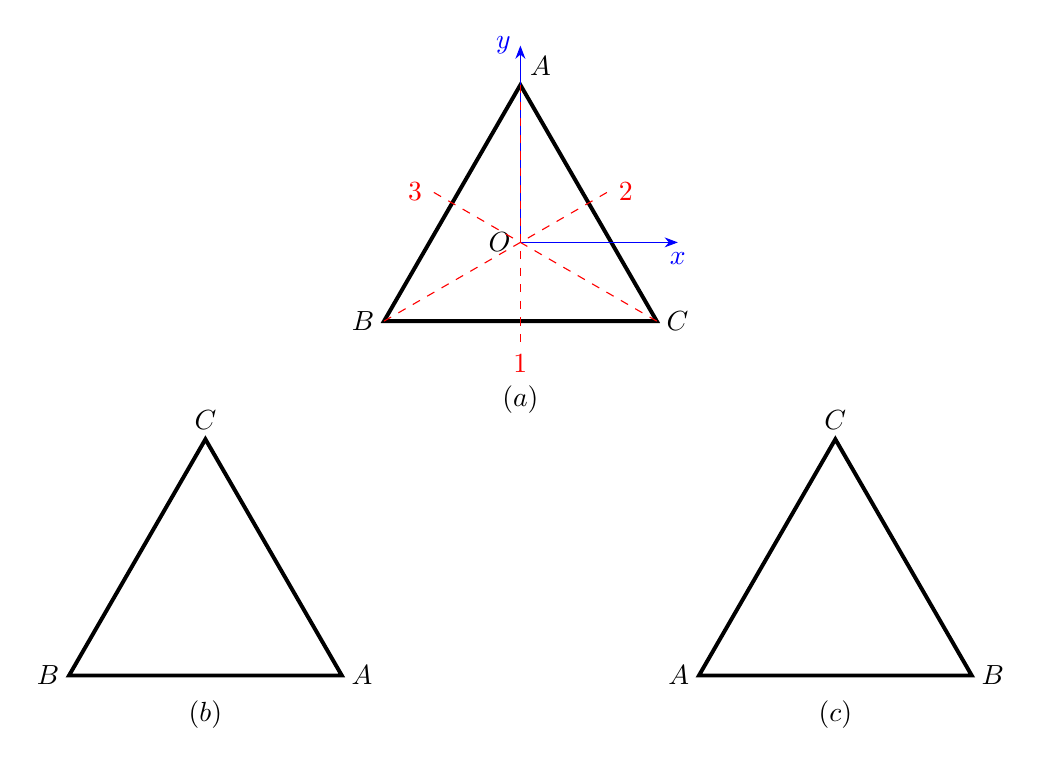
\begin{tikzpicture}
			\draw	[line width=.05cm]	(-1.732, -1) -- (1.732, -1) -- (0, 2) -- cycle;
			\node	(A)	at	(0, 2)			[above right]	{$A$};
			\node	(B)	at	(-1.732, -1)	[left]			{$B$};
			\node	(C)	at	(1.732, -1)		[right]			{$C$};
			\node	(O)	at	(0, 0)			[left]			{$O$};
			\draw	[-Stealth, blue]	(0, 0)		 --	(2, 0)		node[at end, below]{$x$};
			\draw	[-Stealth, blue]	(0, 0)		 --	(0, 2.5)	node[at end, left]{$y$};
			\draw	[red, dashed](0, 2) -- +(0, -3.3)	node[at end, below]{$1$};
			\draw	[red, dashed](-1.732, -1) -- +(30:3.3cm)	node[at end, right]{$2$};
			\draw	[red, dashed](1.732, -1) -- +(150:3.3cm)	node[at end, left]{$3$};
			\node	(a)	at	(0, -2)						{$(a)$};

			\draw	[line width=.05cm]	(-5.732, -5.5) -- (-2.268, -5.5) -- (-4, -2.5) -- cycle;
			\node	(A1)	at	(-2.268, -5.5)	[right]	{$A$};
			\node	(B1)	at	(-5.732, -5.5)	[left]	{$B$};
			\node	(C1)	at	(-4, -2.5)		[above]	{$C$};
			\node	(b)		at	(-4, -6)				{$(b)$};
			\draw	[line width=.05cm]	(2.268, -5.5) -- (5.732, -5.5) -- (4, -2.5) -- cycle;
			\node	(A2)	at	(2.268, -5.5)	[left]	{$A$};
			\node	(B2)	at	(5.732, -5.5)	[right]	{$B$};
			\node	(C2)	at	(4, -2.5)		[above]	{$C$};
			\node	(c)		at	(4, -6)				{$(c)$};
		\end{tikzpicture}
		\caption{正三角形转动操作}
		\label{fig:D3_group_fig}
	\end{figure}
	我们发现,对图中的三角形进行上述任意的六种操作以及相应的乘法操作,此\uline{三角形在空间上保持不变},如图\ref{fig:D3_group_fig}(b),它可以认为是直接对(a)进行$b$操作,也可认为是先进行$c$操作在进行$d$操作,这样,我们就可以得到这样的关系$dc=b$。在这些乘法作用下,上述这些操作构成群,我们称为\textcolor{red}{$D_3$群},其乘法表如下:
	\begin{table}[!ht]
		\centering
		\caption{$D_3$群乘法表}
		\setlength{\tabcolsep}{10mm}{
		\begin{tabular}{|c|cccccc|}\hline
			~	&	e	&	d	&	f	&	a	&	b	&	c	\\	\hline
			e	&	e	&	d	&	f	&	a	&	b	&	c	\\	
			d	&	d	&	f	&	e	&	c	&	a	&	b	\\	
			f	&	f	&	e	&	d	&	b	&	c	&	a	\\	
			a	&	a	&	b	&	c	&	e	&	d	&	f	\\	
			b	&	b	&	c	&	a	&	f	&	e	&	d	\\	
			c	&	c	&	a	&	b	&	d	&	f	&	e	\\	\hline
		\end{tabular} 
		}
	\end{table}
\end{example}


\section{群表示}
\subsection{群表示基础}
构成群的是一些操作,既然是一些操作,那么必然有其所对应的操作对象,其操作对象是位于某一空间下的,比如前面的例\ref{exp:D3_group},群元是一些操作,而这些操作所对应的对象则是位于三维空间中的正三角形;我们将此三角形在三维空间中表示出来(只表示其顶点坐标),那么它将以列矢的形式表现出来,而对应的群操作的表现形式则为矩阵,这些矩阵同样构成群。因此,我们可以说,\CJKunderdot{所谓的群表示就是某一群$G$到线性空间$V$上的某一线性变换群$L(V,C)$的同态映射,也就是说表示是一种同态映射关系,它存在于一个抽象群和线性空间的线性变换群之间。}

群中的群元是对某一个对象进行某种操作,而群表示则相当于我们要在某一个具体的空间下用数学的语言来描述这个群元所对应的操作。在理解这个操作之前需要了解线性空间和线性变换的概念。
\begin{definition}{线性空间(向量空间)}
	线性空间是定义在数域$\mathbb{K}$(比如实数域$\mathbb{R}$或复数域$\mathbb{C}$)上的向量集合$V = \{\bm{x}, \bm{y}, \bm{z}, \cdots\}$。在$V$中可以定义加法和数乘两种运算。设矢量$\bm{x}, \bm{y}, \bm{z} \in V$,数$a , b , c \in \mathbb{K}$,向量加法和数乘都具有封闭性,满足\newline
	向量加法:
	\begin{enumerate}
		\item $\bm{x} + \bm{y} = \bm{y} + \bm{x}$
		\item $\bm{x} + ( \bm{y} + \bm{z} ) = (\bm{x} + \bm{y}) + \bm{z}$
		\item 有唯一$\bm{0}$元素,$\bm{x} + \bm{0} = \bm{x}$
		\item 对$\forall \bm{x}$,有唯一的$-\bm{x}$,使得$\bm{x} + (-\bm{x}) = \bm{0}$
	\end{enumerate}
	向量与数的乘法:
	\begin{enumerate}
		\item $1 \cdot \bm{x} = \bm{x}$
		\item $(ab)\bm{x} = a(b\bm{x})$
		\item $a(\bm{x} + \bm{y}) = a\bm{x} + a\bm{y}$
		\item $(a + b) \bm{x} = a\bm{x} + b\bm{x}$
	\end{enumerate}
	现在把向量的加法看成群的乘法,则线性空间$V$构成一个可交换的加法群。
\end{definition} 
线性空间最简单的一个例子就是三维空间,若三维空间按笛卡尔坐标系展开,则上面的向量都可用$(x, y, z)$表示,而且具有封闭性,也就是这些向量相加或数乘都无法超过这个空间。
\begin{definition}{线性无关向量}
	线性空间$V$中,若任意$n$个向量$\bm{X}_1, \bm{X}_2, \cdots, \bm{X}_n$的线性组合$a_1\bm{X}_1 + a_2\bm{X}_2 + \cdots + a_n\bm{X}_n = 0$,其中$a_1, a_2, \cdots, a_n \in \mathbb{K}$,当且仅当$a_1 = a_2 = \cdots = a_n = 0$时成立,这时,称$\bm{X}_1, \bm{X}_2, \cdots, \bm{X}_n$这些向量线性无关。否则,称他们线性相关。
\end{definition} 

\begin{definition}
	线性变换$A$是将线性空间$V$映入$V$的映射,这个映射对$\forall \bm{x}, \bm{y} \in V$和$\forall a, \in \mathbb{K}$,满足$A(a\bm{x} + b\bm{y} = aA\bm{x} + bA\bm{y}$,也就是说这个变换作用到向量的线性组合上,等于这个变换作用到向量上的线性组合。
\end{definition}
所谓映射其实就是一种操作,它把某个区域的东西变成另一个区域的某样东西,上面的定义中$A$是将$V$中的某个元素变成$V$中的另一样元素,这两个元素可能相同也可能不同。这里,$A$将表现为矩阵形式,而我们所需要做的就是找到$A$所对应的矩阵。当我们取定$V$中的基矢为$\bm{e}_1, \bm{e}_2, \cdots, \bm{e}_n$时,对$V$中的某一向量$x=\sum_{i=1}^{n}x_i\bm{e}_i$做相关的线性变换,表现为
\begin{equation}
	\begin{aligned}
		A\bm{x} =& \sum_{j=1}^{n} x_j A \bm{e}_j = \sum_{j=1}^{n}\sum_{i=1}^{n} x_j e_i a_{ij}	\\
				=& (\bm{e}_1, \bm{e}_2, \cdots, \bm{e}_n)
					\begin{pmatrix}
						a_{11}	&	a_{12}	&	\cdots	&	a_{1n}	\\
						a_{21}	&	a_{22}	&	\cdots	&	a_{2n}	\\
						\vdots	&	\vdots	&	\ddots	&	\vdots	\\
						a_{1n}	&	a_{2n}	&	\cdots	&	a_{nn}	\\
					\end{pmatrix}
					\begin{pmatrix}
						x_1	\\
						x_2	\\
						\vdots	\\
						x_n
					\end{pmatrix}	\label{eq:group_basis_change}
	\end{aligned}
\end{equation}
我们知道,一个线性空间可选取不同的基矢,不同基矢之间可通过矩阵变换联系起来,上式第三个等号的左边两项可构成向量空间$V$的另一组基,我们考虑为$\bm{e}^{\prime}_1, \bm{e}^{\prime}_2, \cdots, \bm{e}^{\prime}_n$,它们之间的关系如下:
\begin{equation}
	\bm{e}^{\prime}_{j} = (\bm{e}_1, \bm{e}_2, \cdots, \bm{e}_n) 
						\begin{pmatrix}
							a_{1j}	\\
							a_{2j}	\\
							\vdots	\\
							a_{nj}
						\end{pmatrix}
\end{equation} 
下面,我们取$V$中另一向量$\bm{y} = \sum_{i=1}^{n}y_i\bm{e}_i$,它是$\bm{x}$通过映射$A$得到的,满足$\bm{y} = A\bm{x}$。对于$\bm{y}$,写成矩阵形式为
\begin{equation}
	\bm{y} = (\bm{e}_1, \bm{e}_2, \cdots, \bm{e}_n)
				\begin{pmatrix}
					y_1	\\
					y_2	\\
					\vdots	\\
					y_n
				\end{pmatrix}	\label{eq:group_basis_eq_change}
\end{equation} 
由于$\bm{y}$与$A\bm{x}$表示的是同一向量,联合式\eqref{eq:group_basis_change}和\eqref{eq:group_basis_eq_change},我们有以下关系成立
\begin{equation}
	 (\bm{e}_1, \bm{e}_2, \cdots, \bm{e}_n)
		\begin{pmatrix}
			a_{11}	&	a_{12}	&	\cdots	&	a_{1n}	\\
			a_{21}	&	a_{22}	&	\cdots	&	a_{2n}	\\
			\vdots	&	\vdots	&	\ddots	&	\vdots	\\
			a_{1n}	&	a_{2n}	&	\cdots	&	a_{nn}	\\
		\end{pmatrix}
		\begin{pmatrix}
			x_1	\\
			x_2	\\
			\vdots	\\
			x_n
		\end{pmatrix}
		=
		(\bm{e}_1, \bm{e}_2, \cdots, \bm{e}_n)
		\begin{pmatrix}
			y_1	\\
			y_2	\\
			\vdots	\\
			y_n
		\end{pmatrix}
\end{equation} 
由式\eqref{eq:group_basis_eq_change},我们用新基矢$\bm{e}^{\prime}_1, \bm{e}^{\prime}_2, \cdots, \bm{e}^{\prime}_n$替换上式等号的右边两个矩阵,也就是有下式成立
\begin{equation}
	(\bm{e}^{\prime}_1, \bm{e}^{\prime}_2, \cdots, \bm{e}^{\prime}_n )
	=
	(\bm{e}_1, \bm{e}_2, \cdots, \bm{e}_n)
	\begin{pmatrix}
		a_{11}	&	a_{12}	&	\cdots	&	a_{1n}	\\
		a_{21}	&	a_{22}	&	\cdots	&	a_{2n}	\\
		\vdots	&	\vdots	&	\ddots	&	\vdots	\\
		a_{1n}	&	a_{2n}	&	\cdots	&	a_{nn}	\\
	\end{pmatrix}
\end{equation} 
以上我们可以看出,通过矩阵$A$,我们可以把新基矢与旧基矢联系起来,矩阵的第$j$列,是新基矢用旧基矢表示的展开系数。这样,当我们知道新基矢与旧基矢之间的关系时(也就是\CJKunderdot{新基矢用旧基矢展开的展开系数}),我们就可以把矩阵$A$写出来,也就是可以把抽象群元对应的表示写出来。我们来看一个例子
\begin{example}
	以$D_3$群群元$b$为例,来考虑它在三维线性空间中的表示。首先,轴$2$在此空间中可表示为某一直线方程:
	\begin{equation}
	    -\tan \frac{\pi}{6} x + y = 0
	\end{equation} 
	而群元$b$是让三角形发生关于此直线的镜像变换,而原来的基矢为$\bm{e}_{x}, \bm{e}_{y}, \bm{e}_z$,变换后的基矢为$\bm{e}^{\prime}_x, \bm{e}^{\prime}_y,\bm{e}^{\prime}_z$,它们之间的关系由下图表示
	\begin{figure}[htbp]
		\centering
		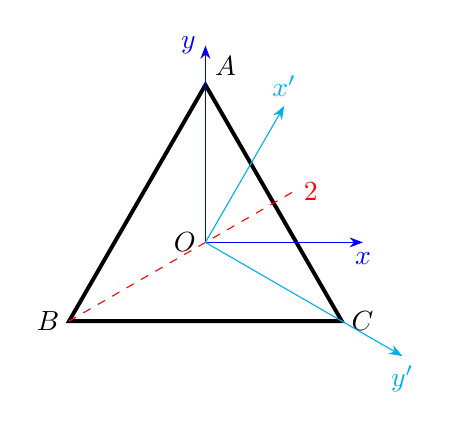
\begin{tikzpicture}
			\draw	[line width=.05cm]	(-1.732, -1) -- (1.732, -1) -- (0, 2) -- cycle;
			\node	(A)	at	(0, 2)			[above right]	{$A$};
			\node	(B)	at	(-1.732, -1)	[left]			{$B$};
			\node	(C)	at	(1.732, -1)		[right]			{$C$};
			\node	(O)	at	(0, 0)			[left]			{$O$};
			\draw	[-Stealth, blue]	(0, 0)		 --	(2, 0)		node[at end, below]{$x$};
			\draw	[-Stealth, blue]	(0, 0)		 --	(0, 2.5)	node[at end, left]{$y$};
			\draw	[red, dashed](-1.732, -1) -- +(30:3.3cm)	node[at end, right]{$2$};

			\draw	[-Stealth, cyan]	(0, 0)		 --	(1, 1.732)		node[at end, above]{$x^\prime$};
			\draw	[-Stealth, cyan]	(0, 0)		 --	(2.5, -1.4434)	node[at end, below]{$y^\prime$};
		\end{tikzpicture}
		\caption{$D_3$群群元$b$在三维空间中的操作}
	\end{figure}
	\newline
	写成数学表达式:
	\begin{equation}
	    \begin{aligned}
			\bm{e}_x^\prime =& \cos \frac{2\pi}{6} \bm{e}_x + \sin \frac{2\pi}{6} \bm{e}_y	\\
			\bm{e}_y^\prime =& \sin \frac{2\pi}{6} \bm{e}_x - \cos \frac{2\pi}{6} \bm{e}_y	\\
			\bm{e}_z^\prime =& \bm{e}_z
	    \end{aligned}
	\end{equation} 
	根据上式写成矩阵形式,则可得到$D_3$群元$b$在三维线性空间中的群表示
	\begin{equation}
	    A(b) =
		\begin{pmatrix}
			\cos \frac{2\pi}{6}	&	\sin \frac{2\pi}{6}		&	0	\\
			\sin \frac{2\pi}{6}	&	-\cos \frac{2\pi}{6}	&	0	\\
			0					&	0						&	1	
		\end{pmatrix}
	\end{equation} 
\end{example}

\begin{definition}
	设有群$G$,如存在一个从$G$到$n$维线性空间$V$上的线性变换群$L(V,C)$的同态映射$A$,则称$A$是群$G$的一个线性表示,$V$为表示空间,$n$是表示的维数。显然,由同态的定义,$\forall g_\alpha \in G$,有$A(g_\alpha) \in L(V, C)$,同时,对$\forall g_\alpha, g_\beta \in G$,有$A(g_\alpha g_\beta) = A(g_\alpha)A(g_\beta)$。$G$的单位元素对应的是$V$上的恒等变换,互逆元素对应的是互逆的变换。
\end{definition}
\CJKunderdot{对于线性空间$V$,如果选定一组特定的基矢,那么每个线性变换都可以有一个矩阵表示,而线性变换也会对应到一个矩阵群。这是,抽象群$G$与线性变换群的同台映射关系可以理解为抽象群$G$与矩阵群的同态映射关系。}我们考虑一个例子来理解这个概念,同样取例\ref{exp:D3_group},我们在三维笛卡尔坐标系中对其展开描述,$D_3$群群元对应到线性空间中的矩阵为
\begin{equation*}
	\begin{aligned}
		&e \xRightarrow[]{A}
		A(e) = 
		\begin{pmatrix}
			1	&	0	&	0	\\
			0	&	1	&	0	\\
			0	&	0	&	1
		\end{pmatrix}
		\\
		&d \xRightarrow[]{A}
		A(d) =
		\begin{pmatrix}
			\cos \frac{2\pi}{3}	&	\sin \frac{2\pi}{3}	&	0	\\
			-\sin	\frac{2\pi}{3}	&	\cos \frac{2\pi}{3}	&	0	\\
			0	&	0	&	1
		\end{pmatrix}
		\\
		&f \xRightarrow[]{A}
		A(d) =
		\begin{pmatrix}
			\cos  \frac{4\pi}{3}	&	\sin \frac{4\pi}{3}	&	0	\\
			-\sin \frac{4\pi}{3}	&	\cos \frac{4\pi}{3}	&	0	\\
			0						&	0					&	1
		\end{pmatrix}
		\\
		&a \xRightarrow[]{A}
		A(a) =
		\begin{pmatrix}
			-1	&	0	&	0	\\
			0	&	1	&	0	\\
			0	&	0	&	1
		\end{pmatrix}
		\\
		&b \xRightarrow[]{A}
		A(b) =
		\begin{pmatrix}
			\frac{1}{2}			&	\frac{\sqrt{3}}{2}	&	0	\\
			\frac{\sqrt{3}}{2}	&	-\frac{1}{2}		&	0	\\
			0					&	0					&	1
		\end{pmatrix}
		\\
		&c \xRightarrow[]{A}
		A(c) =
		\begin{pmatrix}
			\frac{1}{2}			&	-\frac{\sqrt{3}}{2}	&	0	\\
			-\frac{\sqrt{3}}{2}	&	-\frac{1}{2}		&	0	\\
			0					&	0					&	1
		\end{pmatrix}
	\end{aligned}
\end{equation*} 
其中,$A$是一种映射关系,它将$D_3$群中的群元在线性空间中表示为矩阵,而这些矩阵是属于线性变换群$L(V,C)$的。这样,我们可以把群表示关系(抽象群与矩阵变换群的关系)写成如下形式:
\begin{figure}[htbp]
	\centering
	\begin{tikzpicture}
		\draw	(-3, 0)ellipse [x radius=1.2cm, y radius=2cm];
		\draw	(3, 0)ellipse [x radius=1.2cm, y radius=2cm];
		\draw	[-Stealth]	(-2.8, 0.7)	--	(2.8, 0.7);
		\node	(g_alpha)	at	(-2.9, 0.7)	[left]	{$g_{\alpha}$};
		\node	(A_alpha)	at	(2.9, 0.7)	[right]	{$A(g_\alpha)$};
		\node	(G)	at	(-3, 2.5)	{$G$};
		\node	(L)	at	(3, 2.5)	{$L(V,C)$};
		\node	(A)	at	(0, 2.5)	{$A$};
	\end{tikzpicture}
	\caption{群表示}
\end{figure}
\newline
下面,我们举一些例子一边更好的理解清楚这个定义的概念
\begin{example}
	考虑三个二阶群:(1) $\{E, \sigma_k\}$(三维空间对$x-y$平面的反射),(2) $\{E, C_k(\pi)\}$(绕$z$轴转$\pi$角),(3) $\{E, I\}$(空间反演操作)。去表示空间为三维实空间,基矢为$\{\bm{i}, \bm{j}, \bm{k}\}$,写出它们的表示。首先,我们考虑群元$E$,由于它是恒等变换,也就是把$\{\bm{i}, \bm{j}, \bm{k}\}$变成$\{\bm{i}, \bm{j}, \bm{k}\}$,对应的新向量在旧基矢组下的展开系数分别为$(1, 0, 0), (0, 1, 0), (0, 0, 1)$,表示矩阵为三阶单位矩阵。
	\newline
	对于非单位元,考虑第一种情况,$\sigma_k$把$\{\bm{i}, \bm{j}, \bm{k}\}$变为$\{\bm{i}, \bm{j}, -\bm{k}\}$表示矩阵为$ \begin{pmatrix}
		1	&	0	&	0	\\
		0	&	1	&	0	\\
		0	&	0	&	-1
	\end{pmatrix}$;
	\newline
	第二种情况$C_k(\pi)$把$\{\bm{i}, \bm{j}, \bm{k}\}$变为$\{-\bm{i}, -\bm{j}, \bm{k}\}$,表示矩阵为$ \begin{pmatrix}
		-1	&	0	&	0	\\
		0	&	-1	&	0	\\
		0	&	0	&	1
	\end{pmatrix}$;
	\newline
	第三种情况$I$把$\{\bm{i}, \bm{j}, \bm{k}\}$变为$\{-\bm{i}, -\bm{j}, -\bm{k}\}$,表示矩阵为$ \begin{pmatrix}
		-1	&	0	&	0	\\
		0	&	-1	&	0	\\
		0	&	0	&	-1
	\end{pmatrix}$。
\end{example}

我们需要弄清楚的一点是,\textcolor{red}{抽象群的群元是作用在向量$\bm{r}$上的,而群元的表示是作用在基矢上的,我们以什么作为基矢,那么表示就作用在谁身上,而有时候向量和基矢的类型可能是不一样的}。上面的例子中,我们很容易理解抽象群群元作用在了一个变量$\bm{r}$上,由于我们选取的基矢也是向量,所以这些群元的表示也作用在向量上;而对于一些基矢为函数的情况则有所不同,当我们选取函数$\{\Psi_1(\bm{r}), \Psi_2(\bm(r), \cdots, \Psi_n(\bm{r}))\}$作为基矢时,抽象群群元$g_i$仍作用在$\bm{r}$上,但是其表示$A(g_i)$却是作用在$\Psi_i(\bm{r})$上的。

我们以$\Psi_i(\bm{r})$为例,$g_\alpha$作用到基矢$\Psi_i(\bm{r})$上的效果为$ g_\alpha \Psi_i(\bm{r}) =\Psi_i(g_\alpha \bm{r}) = \Psi_i(\bm{r}^{\prime})$;$A(g_\alpha)$作用到$\Psi_i(\bm{r})$上的效果为:$ A(g_\alpha)\Psi_i(\bm{r}) = \Psi_i^{\prime}(\bm{r})$。由于$A(g_\alpha)$是群元$g_\alpha$的表示,也就是有关系$\Psi_i(g_\alpha \bm{r}) = A(g_\alpha)\Psi_i(\bm{r})$成立,所以最后得到的结果应该也要保持一致,所以应该满足关系:$\Psi_i^\prime(\bm{r}) = \Psi_i(\bm{r}^\prime)$。现在,$\Psi^\prime_i(\bm{r})$变成了新的基矢,基于前面的讨论,我们如果想要知道表示$A(g_\alpha)$的具体形式,我们只要将新基矢$\Psi_i^{\prime}(\bm{r})$用旧基矢$\Psi_i(\bm{r})$进行展开,并得到对应的展开系数便能求得$A(g_\alpha)$,等价的,我们只需要将$\Psi_i(\bm{r}^\prime)$进行展开便可以得到$\Psi^\prime_i(\bm{r})$的展开结果。

\subsection{等价表示,可约表示,酉表示}
\begin{definition}{等价表示}
	设群$G=\{g\}$在表示空间上的一个表示$A$是$\{A(g_\alpha)$,也就是说对每个$g_\alpha$都有非奇异变换$A(g_\alpha)$与之对应。设$P$是$V$上的一个非奇异变换,${\rm det}(P)$不为零,则$\{P^{-1} A(g_\alpha) P\}$也给出群$G$的一个表示,因为每个$g_\alpha$也唯一对应一个$\{P^{-1}A(g_\alpha)P\}$,且$\{P^{-1}A(g_\alpha)P\}$
\end{definition}

\subsection{有限群表示理论}
\begin{theorem}{完备性定理}
	设$A^{p}(p = 1, 2, \cdots, q)$是有限群$G = {g_{\alpha}}$的所有不等价不可约酉表示,则$A^{p}$生成的群函数$A^{p}_{\mu\nu}(g_{i})$在$p$遍历所有不等价不可约酉表示的指标,$\mu, \nu$遍历所有行和列的指标时,$A^{p}_{\mu\nu}(g_{i})$在群函数空间是完备的。
\end{theorem} 
下面我们来证明此定理:
\begin{proof}
	我们需要用到一些简单的性质:假设有一个群空间,我们按群代数中定义的向量乘法来做线性变换时,这个群空间是右正则表示$R(g_j)$的表示空间。
\end{proof}

\begin{problemset}[习题]
\item 设$A(g)$群$G=\{g\}$的一个表示,证明:复共轭$A^{*}(g)$也是$G$的一个表示。如果$A(g)$是不可约的或酉的,那么$A^*(g)$也是不可约的或酉的。
	\begin{proof}
		$A(g)$是群$G$的一个表示,存在这样一个表示空间$V$,使$A(g)$与此空间上的一般线性变换群$L(V,C)$同态,即对$\forall g_i$,我们有$A(g_i) \in L(V, C)$成立,且满足
		\begin{equation*}
			\begin{aligned}
				\forall g_{i} \in G, \quad & A(g_i) \in L(V, C)	\\
				\forall g_{i}, g_{j} \in G, \quad & A(g_i g_j) = A(g_i) A(g_j) \in L(V, C)
			\end{aligned}
		\end{equation*}
		对于复共轭$A^*(g)$,我们可以取表示空间$V$上的一般线性变换群$L^* (V, C)$,使其满足$\forall A^* (g_i) \in L^* (V, C)$,并且,我们有对$\forall g_i \in G, A^*(g_i) \in L^*(V, C)$,且有以下关系:
		\begin{equation*}
			\begin{aligned}
				& A^* (g_i g_j) = [A(g_i) A(g_j)]^* = A^*(g_i) A^*(g_j) \in L^* (V, C)	\\
				& A^{*}(e) \in L^{*}(V, C) \\
				& A^{*}(g) A^{-1*}(g) = [A(g)A^{-1}(g)]^* = E^* = E
			\end{aligned}
		\end{equation*} 
		可知,$A^{*}(g)$同样满足群表示的定义,也是群$G$的一个表示。
	\end{proof}
\end{problemset}



%%%%%%%%%%%%%%%%%%%%%%%%%%%%%%%%%%%%%%%%%%%%%%%%
\part{理论力学}
\chapter{力学基本原理}

%%%%%%%%%%%%%%%%%%%%%%%%%%%%%%%%%%%%%%%%%%%%%%%%%%%%%%%%%%%%%%%%%%%%%%%%%%%%%%%%%%
\section{单粒子力学原理}
\begin{theorem}[单粒子守恒原理]
	线动量守恒:若合力$\bm{F} = 0$, 即$\bm{\dot{p}} = 0$,则线动量$\bm{p}$守恒。
\end{theorem}
考虑一个单粒子运动,其位置矢量表示为$\bm{r}$,对应的速度为
\begin{equation}
  \bm{v} = \frac{d \bm{r}}{d t} \label{eq_single_velocity}
\end{equation}
粒子质量为$m$,则其动量定义为:
\begin{equation}
  \bm{p} = m \bm{v}   \label{eq_single_momentum}
\end{equation}
其方向与速度方向一致。由于粒子可能与外部物体或场发生相互作用,因此粒子会受到外部力的作用,粒子所受到的合力可以写为;
\begin{equation}
  \bm{F} = \frac{d \bm{p}}{dt} = \dot{\bm{p}} = \frac{d }{dt}(m\bm{v})  \label{eq_single_tot_force}
\end{equation}
在质量守恒的情况下,上式可写为:
\begin{equation}
  \bm{F} = m \frac{d\bm{v}}{dt} m \bm{a}
\end{equation}
其中$\bm{a}$为粒子的矢量加速度,其定义为
\begin{equation}
	\bm{a} = \frac{d^2 \bm{r}}{dt^2}
\end{equation}
此运动方程仅为二阶微分方程,假设$\bm{F}$并不依赖于高阶微分项。
\begin{definition}{惯性系(伽利略系)}
	在惯性系中,对于不受合外力影响的物体将保持相对静止或匀速直线运动,其时间是均匀流逝的,空间也是均匀且各向同性的。此参考系使方程\eqref{eq_single_tot_force}成立。
\end{definition}

\vspace{5pt}
\begin{theorem}{角动量守恒原理}
	若一物体的总扭矩$\bm{N}=0$,即角动量$\bm{L}$对时间的一次微分项$\dot{\bm{L}} = 0$,则粒子的角动量$\bm{L}$守恒,也就是总角动量$\bm{L}$不随时间变化。
\end{theorem}
若粒子绕某一点$O$旋转,其与点$O$的径矢为$\bm{r}$,动量为$\bm{p}$,可定义其角动量为
\begin{equation}
	\bm{L} = \bm{r} \times \bm{p}	\label{eq_angular_momentum}
\end{equation}
类似公式\eqref{eq_single_tot_force},定义该粒子关于某一点的\underline{\textit{力矩}}为
\begin{equation}
	\bm{N} = \frac{d\bm{L}}{dt} = \frac{d \bm{r}}{dt} \times \bm{p} + \bm{r} \times \frac{d\bm{p}}{dt} = \bm{v} \times (m\bm{v}) + \bm{r} \times \frac{d\bm{p}}{dt} = \bm{r} \times \frac{d(m\bm{v})}{dt} = \bm{r} \times \bm{F}
\end{equation}
显然,我们可以得到力矩与角动量之间的关系为:
\begin{equation}
	\bm{N} = \frac{d\bm{L}}{dt} = \dot{\bm{L}}
\end{equation}
\begin{note}
	需要注意的是,$\bm{L}$和$\bm{N}$都依赖于点$O$。
\end{note}

\vspace{5pt}
\begin{theorem}{能量守恒原理}
	若作用在一个粒子上的力是保守的,那么这个粒子的总能量(总动能+势能) $T+V$是守恒的。
\end{theorem}
考虑一个粒子在外力$\bm{F}$作用下从点$1$到点$2$所做的功。
\begin{equation}
	W_{12} = \int_{1}^{2} \bm{F} \cdot d\bm{s}	\label{eq_work_done}
\end{equation}
若质量为常量(若无特殊说明,第一部分中质量皆为常数),则方程\eqref{eq_work_done}可约化为:
\begin{equation}
	\int_{1}^{2} \bm{F} \cdot d\bm{s} = m \int \frac{d\bm{v}}{dt}\bm{v} dt = \frac{m}{2} \int \frac{d}{dt}(v^2) dt = \frac{m}{2} \int \frac{d(v^2)}{dt} 
\end{equation}
因此,我们有
\begin{equation}
	W_{12} = \frac{m}{2}(v_2^2 - v_1^2)
\end{equation}
其中,标量$mv^2/2$表示该粒子的动能,并用$T$标记,则上式可改写为
\begin{equation}
	W_{12} = T_2 - T_1	\label{eq_tot_different_kinetic}
\end{equation} 
上式表示在外力$\bm{F}$的作用下,粒子从位置1到位置2的动能变化。
\begin{note}
	\underline{力场保守},也就是该力场下使粒子从点1沿任意路径运动到点2,其所作功$W_{12}$不变;换种说法,若力场保守,则粒子从起点出发沿任意闭合路径在运动回起点,所作功为0,即满足下式
	\begin{equation}
		\oint \bm{f} d\bm{s} = 0	\label{eq_force_circuit_path}
	\end{equation} 
	可类比于重力场,我们在不考虑其他外力的作用下,一个物体从地面运动到楼顶在回到地面,重力对它是不做功的。
\end{note}
$W_{12}$与路径无关的的充要条件是该粒子受力为某一标量坐标函数的梯度:
\begin{equation}
	\bm{F} = - \nabla V(\bm{r})	\label{eq_force_derived_potential}
\end{equation} 
其中,$V$就是所谓的势,或者称为势能。若$W_{12}$与路径无关,仅与两个终点有关,那么它对路径的微分应该表现为一个常量,这个常量应该可以由$-V$对路径的微分进行确定,或该常量与路径微分的标积等于$-V$的微分:
\begin{equation*}
	\bm{F} \cdot d \bm{s} = -d V  \quad \text{or} \quad F_{s} = \frac{\partial V}{\partial s}
\end{equation*} 
上式与方程\eqref{eq_force_derived_potential}是一致的。
\begin{note}
	注意到式\eqref{eq_force_derived_potential},方程左边加入任意一个常量其结果不变,因此可以知道,零势能面是可以任意确定的。
\end{note}
对于一个守恒的系统,从点1到点2的所作的功可用势能之差表示,如下:
\begin{equation}
	W_{12} = V_2 - V_1	\label{eq_work_down_v}
\end{equation} 
由式\eqref{eq_tot_different_kinetic}和\eqref{eq_work_down_v}可得如下关系:
\begin{equation}
	T_1 + V_1 = T_2 + V_2	\label{eq_energy_conservation}
\end{equation} 
上式表示,在一个守恒体系下,系统在某一点出的动能与势能之和等于某一常数。

%%%%%%%%%%%%%%%%%%%%%%%%%%%%%%%%%%%%%%%%%%%%%%%%%%%%%%%%%%%%%%%%%%%%%%%%%%%%%%%%%%
\section{约束}
\paragraph*{约束的分类:}
\begin{enumerate}
	\item 完整约束(holonomic):其具有以下形式
		\begin{equation}
			f(\bm{r}_1, \bm{r}_2,\cdots, \bm{r}_n, t) = 0	\label{eq_constrain_holo}
		\end{equation} 
		例如刚体,刚体系统中每个点之间的距离是固定的,有如下形式:
		\begin{equation*}
			(\bm{r}_i - \bm{r}_j)^2 - c_{ij}^2 = 0
		\end{equation*} 
		此形式的方程就是具有完整约束的约束方程。	
	\item 非完整约束(nonholonomic),无法将约束形式写为方程\eqref{eq_constrain_holo}的形式,例如在空心球内的气体运动:
		\begin{equation*}
			\bm{r} - a^2 = 0
		\end{equation*} 
\end{enumerate}
此外,还可根据约束中是否包含时间来进行划分,约束中显示的包含时间则将此约束类型称为非恒稳约束(rheonomous),约束中不包含时间则为恒稳约束(scleronomous)。

此外,约束也可能带来一些问题,如下:
\begin{enumerate}
	\item 受约束方程的影响,粒子坐标不再独立,而这会使每个粒子的运动方程发生联系;
	\item 在很多问题的求解中需要知道约束力,而这往往是未知的。
\end{enumerate}

\vspace{5pt}
下面介绍一下\underline{广义坐标}:我们需要先了解一下什么是\underline{自由度}。在笛卡尔坐标系中,描述一个自由粒子的确切位置可用$(x,y,z)$三个坐标来标定,这三个坐标之间无关联关系,我们成这个粒子具有三个自由度;此时,我们再考虑一个具有$N$个自由粒子的系统,此时每个粒子都有一套独立的坐标$(x_1, y_1, z_1), (x_2, y_2, z_2), \cdots (x_n, y_n, z_n)$一共$3N$个独立坐标来标定整个系统的状态,则我们称这个系统具有$3N$个自由度。现在,我们对这个系统施加$k$个完整约束,则对整个系统有$k$个约束方程,对这些方程进行联立则可消掉$k$个自由度,则整个系统只剩下$3N-k$个独立变量,我们将其称为此系统的$3N-k$个自由度,我们用$q_1, q_2, \cdots, q_{3N-k}$来表示,则每个粒子的坐标可以表示为:
\begin{equation*}
	\begin{aligned}
		\bm{r}_1 &= \bm{r}_1(q_1, q_2, \cdots, q_{3N-k})	\\
					   &\cdots	\\
		\bm{r}_N &= \bm{r}_N(q_1, q_2, \cdots, q_{3N-k})	\\
	\end{aligned}
\end{equation*} 
上式称为从$\bm{r}_i$到$q_i$的转换方程。
\begin{note}
	广义坐标一般与三维笛卡尔坐标是不一样的,他们不一定正交,只是互不相关的一些量而已。	
\end{note}

%%%%%%%%%%%%%%%%%%%%%%%%%%%%%%%%%%%%%%%%%%%%%%%%%%%%%%%%%%%%%%%%%%%%%%%%%%%%%%%%%%
\section{虚位移,虚功原理和达朗贝尔原理}
\textbf{\textcolor{red}{虚位移(virtual displacement),也称无穷小位移(infinitesimal displacement)}:}在某一时刻$t$,物体在约束条件下发生的任意无穷小位移。虚位移与实际发生的位移是不一样的,它是物体在受约束情况下可能发生的任何一种无穷小位移,但实际并没发生,而实际位移则是物体真实产生的位移,一般只有一种。举个例子,若一个物体被约束在$Oxy$平面上运动,则其虚位移如下:
\begin{figure}[htbp]
	\begin{center}
	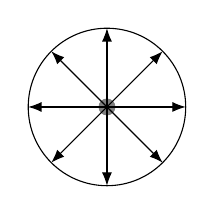
\begin{tikzpicture}[auto]
		\draw	(0, 0)	circle	[radius=1cm];
		\filldraw	[gray]	(0, 0)	circle	[radius=0.1cm];
		\draw	[-Latex]	(0, 0)	-- (0, 1);
		\draw	[-Latex]	(0, 0)	-- (1, 0);
		\draw	[-Latex]	(0, 0)	-- (-1, 0);
		\draw	[-Latex]	(0, 0)	-- (0, -1);
		\draw	[-Latex]	(0, 0)	-- (0.7071, 0.7071);
		\draw	[-Latex]	(0, 0)	-- (-0.7071, 0.7071);
		\draw	[-Latex]	(0, 0)	-- (0.7071, -0.7071);
		\draw	[-Latex]	(0, 0)	-- (-0.7071, -0.7071);
	\end{tikzpicture}
	\end{center}
	\caption{虚位移$\delta \bm{r}$的图像,此时约束力垂直平面向里。}
\end{figure}

\paragraph*{虚功原理:}为推导此原理,我们假设系统处于平衡状态,也就是作用在系统中每一粒子的合力$\bm{F}_i = 0$,因此,系统中每一点的虚功(合外力在虚位移上所做的功)为0,即$\bm{F}_i \cdot \delta \bm{r}_i =0$。对系统中所有粒子的虚功取和,我们同样应该由
\begin{equation}
	\sum_i \bm{F}_i \cdot \delta \bm{r}_i  = 0 \label{eq_system_virtual_work}
\end{equation} 
系统中某一粒子的合力由作用力$\bm{F}^{(a)}_i$和约束力$\bm{f}_i$,对此,式\eqref{eq_system_virtual_work}可化为:
\begin{equation}
	\sum_i \bm{F}^{(a)}_i \cdot + \sum_i \bm{f}_i \cdot \delta i = 0	\label{eq_system_virtual_work_decomposed}
\end{equation} 
现在,我们仅考虑净虚功为0的情况,也就是约束力对所有虚位移所作功之和为0的情况:比如一个物体被约束在某一平面,那么约束力与该平面垂直,而虚位移只能与该平面相切,此时的虚功便为0。在这种情况下,式\eqref{eq_system_virtual_work_decomposed}左边第二项变为0,进一步,我们可以知道其作用力在虚位移上所作的功也为0:
\begin{equation}
	\sum_i \bm{F}^a_i \cdot \delta \bm{r}_i = 0	\label{eq_virtual_work_principle}
\end{equation} 
式\eqref{eq_virtual_work_principle}就是所谓的\underline{\textcolor{red}{虚功原理}}。由于$\bm{r}_i$受约束作用,它们并不独立,因此我们一般有$\bm{F}^{(a)}_i \neq 0$,因此,在具体计算时,我们需要将上述虚位移转化为相互独立的广义坐标$q_i$空间进行计算。
\begin{note}
	若一个粒子被约束在某一平面且存在摩擦,由于约束力总与虚位移垂直,某一时刻的物体在虚位移上所作的虚功仍为0;但是,物体在真实位移上所作功(并不特指约束力所作功)不一定为0,因为摩擦力会作功。
\end{note}

\textbf{达朗贝尔原理(D'Alembert's principle):}上述虚功原理只适合用于系统平衡的情况,当系统处于运动中时,需要使用达朗贝尔原理进行计算。一般的,\textcolor{red}{ 运动方程 }为:
\begin{equation*}
	\bm{F}_i = \dot{\bm{p}}_i
\end{equation*} 
可将上式重新写为:
\begin{equation*}
	\bm{F}_i - \dot{\bm{p}} = 0
\end{equation*}
上式$\bm{f}_i$表示作用在一个粒子上的合外力,减去$\dot{\bm{p}}$后整个式子变为了0,我们将$-\dot{\bm{p}}$称为“相反的有效力”,它与合外力共同作用使此粒子处于平衡态。将上式代入式\eqref{eq_system_virtual_work},并遍历所有粒子,我们有:
\begin{equation}
	\sum_{i}(\bm{F}_i - \dot{\bm{p}}_i) \cdot \delta \bm{r}_i = 0
\end{equation} 
同时,我们按式\eqref{eq_virtual_work_principle}将合力分解为作用力和粒子间作用力,得到
\begin{equation*}
	\sum_i (\bm{F}^{(a)}_i - \dot{\bm{P}}_i \cdot \delta \bm{r}_i + \sum_i \bm{f}_i \cdot \delta \bm{r}_i = 0)
\end{equation*} 
同样,我们只在讨论约束力所作虚功为0的情况,则上式最后可以化为:
\begin{equation}
	\sum_i (\bm{F}^{(a)}_{i} - \dot{\bm{p}}_i) \cdot \delta \bm{r}_i = 0	\label{eq_dalember_principle}
\end{equation} 
称\eqref{eq_dalember_principle}为\underline{达朗贝尔原理(D'Alembert's principle)}。现在,我们知道,当约束力所作虚功为0时,合外力所作功与物体运动加速度产生的所谓“相反有效力”所作功相等,此处,我们可以将上标$^{(a)}$去掉。

\textbf{广义坐标下的达朗贝尔原理:}为方便求解动力学问题,我们需要将达朗贝尔原理用广义坐标来表示。我们将$\bm{r}_i$转换为广义坐标$q{j}$(假设有$n$个独立坐标),其变换方程为:
\begin{equation*}
	\bm{r}_i = \bm{r}_i(q_1, q_2, \cdots , q_n, t)
\end{equation*} 
这样,$\bm{r}_i$对应的速度可以表示为:
\begin{equation*}
	\bm{v}_i \equiv \frac{d\bm{r}_i}{dt} = \sum_k \frac{\partial \bm{r}_i}{\partial q_k} + \frac{\partial \bm{r}_i}{\partial t}
\end{equation*} 
类似地,我们可以得到虚位移$\delta\bm{r}_i$的表示:
\begin{equation*}
	\delta\bm{r}_i = \sum_i \frac{\partial \bm{r}_i}{\partial q_j}\delta q_j
\end{equation*} 
\begin{note}
	虚位移是在某一时刻下物体可能发生的任意无穷小的位移,因此它只是广义坐标的函数,而不包含时间的变化$\delta t$。此外,我们在讨论虚位移时确实也只应该将其当成广义坐标的函数,应该排除其包含时间,因此当约束力随时间变化时,虚位移与约束力应当是相互垂直的。
\end{note}
下面需要引出\textcolor{red}{\underline{广义力}}的概念:在广义坐标下,$\bm{F}_i$表示为
\begin{equation}
	\sum_i \bm{F}_i \cdot \delta \bm{r}_i = \sum_{i, j}\bm{F}_i \cdot \frac{\partial \bm{r}_i}{\partial q_j} \delta q_j = \sum_{j} Q_j \delta q_j
\end{equation} 
其中,$Q_j$就是所谓的\textcolor{red}{广义力},其形式为
\begin{equation}
	Q_j = \sum_{i} \bm{F}_i \cdot \frac{\partial \bm{r}_i}{\partial q_j}	\label{eq_generalized_force}
\end{equation} 
\begin{note}
	广义坐标$q$单位不一定为长度,同样地,广义力$Q$的单位也一定为力的单位,但必须保证他们的乘积具有功的单位。如$q$表示转动的角度$d\theta$而$Q$表示力矩$N_j$,他们的乘积$N_j d\theta$则具有功的单位。
\end{note}






\include{classic-mechan/chapter2.tex}
\chapter{中心力问题}

\section{位力定理}

\chapter{刚体运动的动能}

\section{刚体的独立坐标}

刚体系统具有$N$个粒子,这些粒子间的相对位置是确定的,也就是说对于任意两个粒子$i$和$j$,其相对距离满足
\begin{equation}
	r_{ij} = c_{ij}	\label{eq:rigid-constraint}
\end{equation} 
其中$c_{ij}$是一个常数。这是$N$粒子刚体系统满足的约束方程。确定这样一个系统的空间状态,我们需要确定$N$个粒子的自由度,整个系统总共就有$3N$个自由度,这是非常复杂的,而上式所确定的约束方程总共有$\dfrac{N(N-1)}{2}$个,对于很大的$N$来说,这远远大于了系统的所有粒子的自由度数目,因此上述的约束方程并不是完全独立的。

在确定整个刚体系统的空间位置前,我们先考虑如何确定一个点在空间中的位置。对于空间中一个点$4$的位置,我们可以先确定空间中不同直线上的三个点$1$、$2$、$3$的位置,并且确切地知道点$4$相对于这三个点的距离时,我们就可以唯一确定点$4$的位置。现在考虑多粒子系统的刚体系统,我们可以知道任意一点$i$相对于$1$、$2$、$3$的距离$c_{i1}$、$c_{i2}$、$c_{i3}$,这样,我们基于这三个点就可以确定刚体内其余所有点的位置,也就确定了这个刚体的空间位置。

现在,我们已经把整个刚体的空间位置由$N$个点的自由度约化成了确定$3$个点的自由度问题,下面来定出这$3$个点所需要的自由度个数。首先,我们知道了刚体内所有点的约束条件为式\eqref{eq:rigid-constraint},从而知道这三个点具有确定的相对距离为
\begin{equation*}
	r_{12} = c_{12}, \quad r_{13} = c_{13}, \quad r_{23} = c_{23}
\end{equation*} 
我们确定点$1$需要三个自由度;点$2$在以点$1$为球心,$r_{12}$为半径的球面上,因此我们只需要知道点$2$的两个自由度便可以确定其位置;在确定前两个点的位置后,点$3$位于点$1$和点$2$为球心,$r_{13}$和$r_{23}$为半径的球面相交所构成的圆上,因此,我们只需要确定其中一个自由度就可以知道点$3$的确定位置。综上,我们总共需要确定$3+2+1=6$个自由度便可以最终定下三个点的具体空间位置,再根据刚体内点的约束关系,就可以确定好整个系统的空间位置。

\paragraph*{相对坐标系统:}空间中有一套Cartesian坐标系统,刚体处于这个坐标系统中,称为unprimed坐标系统,单位矢量为$\bf{i}$、$\bf{j}$和$\bf{k}$;在刚体内部建立另一套Cartesian坐标系统,刚体内部的粒子用此坐标系统来标记,称为primed坐标系统,其单位矢量为$\bf{i}^{\prime}$、$\bf{j}^{\prime}$和$\bf{k}^{\prime}$。


\include{classic-mechan/Kinematics_RBM.tex}

%%%%%%%%%%%%%%%%%%%%%%%%%%%%%%%%%%%%%%%%%%%%%%%%
\part{量子力学}
\chapter{角动量理论}
%%%%%%%%%%%%%%%%%%%%%%%%%%%%%%%%%%%%%%%%%%%%%%%%%%%
%%%%%%%%%%%%%%%%%%%%%%%%%%%%%%%%%%%%%%%%%%%%%%%%%%%

\section{角动量}
%%%%%%%%%%%%%%%%%%%%%%%%%%%%%%%%%%%%%%%%%%%%%%%%%%%
\paragraph*{角动量算符} 角动量算符满足的的充要条件如下
\begin{theorem}{角动量算符的充要条件}
	\begin{equation}
		J^{\dagger}_k = J_k, ~ k = 1, 2, 3, \quad \left[J_i, J_j\right] = i\hbar \sum_{k} \epsilon_{ijk} J_k
	\end{equation}
\end{theorem}
其中,$\epsilon_{ijk}$是反对称的三维Levi-Civita排序符号。其有如下性质:1. 若有两个指标相同,则$\epsilon_{ijk} = 0$;2. 若三个指标两两不等,按循环排序,即如下图所示的排序时,有$\epsilon_{123} = \epsilon_{231} = \epsilon_{312} = 0$;3. 剩下的排序将使排序符号为$-1$。
\begin{figure}[htbp]
	\centering
	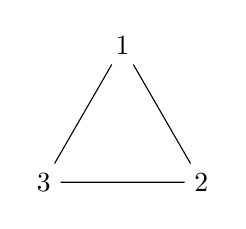
\begin{tikzpicture}
		\node (A) at (0,0) {3};
		\node (B) at (2,0) {2};
		\node (C) at (60:2) {1};
		\draw (A) -- (B) -- (C) -- (A);
	\end{tikzpicture}
\end{figure}

\paragraph*{角动量算符的本征态和本征值} 角动量$\boldsymbol{J}$的本征态和本征值如下
\begin{align}
	\boldsymbol{J}^2 |j\ m\rangle =& j(j+1)\hbar^2 |j\ m\rangle	\\
	J_z |j\ m\rangle =& m\hbar |j\ m\rangle
\end{align}
其正交性和归一性为
\begin{equation}
	\langle j^{\prime}\ m^{\prime} | j\ m\rangle = \delta_{jj^{\prime}}\delta_{mm^{\prime}}, \quad m = -j,\ -j+1, \ \cdots, j-1,\ j \ .
\end{equation}
此外,我们定义角动量的梯度算符
\begin{equation}
	J_{\pm} = J_{x} \pm i J_{y}
\end{equation}
满足对易式
\begin{equation}
	\left[J_{+}, J_{-}\right] = 2\hbar J_z, \quad \left[J_{\pm}, J_{z}\right] = \mp \hbar J_{\pm}
\end{equation}
梯度算符作用到本征态上的效果为
\begin{equation}
	\begin{aligned}
		J_{\pm} |j\ m\rangle =& \hbar \sqrt{j(j+1) - m(m\pm)1} |j\ m\pm 1\rangle	\\
						   =& \hbar \sqrt{(j\pm m +1) (j\mp m)} |j\ m\pm 1\rangle
	\end{aligned}
\end{equation}
对于单粒子在希尔伯特空间中的抽象角动量本征态$|j\ m\rangle$的坐标表示通常为\underline{球谐函数}。

\paragraph*{角动量}

%%%%%%%%%%%%%%%%%%%%%%%%%%%%%%%%%%%%%%%%%%%%%%%%%%%
%%%%%%%%%%%%%%%%%%%%%%%%%%%%%%%%%%%%%%%%%%%%%%%%%%%
\section{角动量耦合}


%%%%%%%%%%%%%%%%%%%%%%%%%%%%%%%%%%%%%%%%%%%%%%%%%%%
\subsection{自旋-轨道耦合}
	自旋轨道耦合

%%%%%%%%%%%%%%%%%%%%%%%%%%%%%%%%%%%%%%%%%%%%%%%%%%%
\subsection{两角动量耦合}
考虑两个完全对易的角动量$\boldsymbol{J}_1$和$\boldsymbol{J}_2$,也就是说这两个角动量分别属于两个不同的粒子,或者是一个粒子的自旋角动量和轨道角动量。


%%%%%%%%%%%%%%%%%%%%%%%%%%%%%%%%%%%%%%%%%%%%%%%%%%%
\subsection{Clebsch-Gordan系数和3-j符号}



%%%%%%%%%%%%%%%%%%%%%%%%%%%%%%%%%%%%%%%%%%%%%%%%%%%

\chapter{正则量子化方法}

\include{quantum-mechan/QuantumHarmonicOscilator.tex}
\chapter{三维空间的量子力学问题}
\section{径向解}
中心势场问题中的径向方程写为如下形式:
\begin{equation}
	\frac{1}{R}\frac{d}{dr}\left(r^2 \frac{dR}{dr}\right) + \left\{\frac{2mr^2}{\hbar^2}[ E-V(r) ]\right\}=  l(l+1)	\label{radial-equation}
\end{equation} 
束缚态下的体系能量呈现分立谱,以下只考虑束缚态情况。

为求解方程\eqref{radial-equation},作函数代换以方便求解:
\begin{equation}
    R(r) = \frac{u(r)}{r}	\label{eq:radial-sub}
\end{equation} 
这样,我们可以得到如下关系:
\begin{equation}
	\begin{aligned}
		\frac{dR}{dr} =& \frac{d}{dr} \left( \frac{u(r)}{r} \right) = \frac{r (du/dr) - u}{r^2}	\\
		\frac{d}{dr}\left( r^2 \frac{dR}{dr} \right)  =& \frac{d}{dr}\left( r \frac{du}{dr} - u \right) = r \frac{d^2u}{dr^2} 
	\end{aligned}
	\label{eq:radila-sub-tran}
\end{equation} 
将式\eqref{eq:radial-sub}、\eqref{eq:radila-sub-tran}代入式\eqref{radial-equation},得到关于$u(r)$的方程,
\begin{equation}
	-\frac{\hbar^2}{2m} \frac{d^2 u}{dr^2} + \left[ V(r) + \frac{\hbar^2}{2m}\frac{l(l+1)}{r^2} \right] u = Eu
\end{equation} 
这个方程与一维薛定谔方程类似,不过势能项有所改变,其中的$\frac{\hbar^2}{2m}\frac{l(l+1)}{r^2}$类似与经典力学中的离心作用,称为离心项。

下面在谐振子势阱下对其进行求解。

\subsection{谐振子势下的径向方程求解}

径向上的球形谐振子势表示为:
\begin{equation*}
	V = \frac{1}{2} \omega^{2} r^{2}
\end{equation*} 



\chapter{波函数和薛定谔方程}
按哥本哈根学派的


%%%%%%%%%%%%%%%%%%%%%%%%%%%%%%%%%%%%%%%%%%%%%%%%
\part{原子核物理}
\chapter{液滴模型}
%%%%%%%%%%%%%%%%%%%%%%%%%%%%%%%%%%%%%%%%%%%%%%%%%%%%%%%%%%%%%%%%%%%%%%%%%%%%%%%%%%
\section{引言}
\textbf{液滴模型(LDM)提出的依据:}
\begin{enumerate}
	\item 原子核的不可压缩性:一般的,我们认为原子核无法的压缩性极低,且其体积不随其形状的改变而发生变化;
	\item 原子核具有明确的表面(well defined surface);
	\item 原子核中核力的\textcolor{red}{\underline{饱和性质:}}原子核中的一个核子仅与有限个核子发生相互作用。
\end{enumerate}

基于上面原子核的性质,人们提出了所谓的液滴模型,将原子核当成一个均匀带电的、不可压缩的、体积不变的液滴。从严格意义上来讲,这与真实的原子核情况是不相符的:原子核还具有结团(cluster)现象,表现为质量数等于4的核较为稳定;此外,在经典液滴中,两粒子的平均距离由粒子间作用力的极小值给出,大约为0.7fm,但是真实原子核应该是一个量子流体,其中的粒子间平均距离约为2.4fm,这是因为核子是满足费米统计(Fermi statistics)的,此时,泡利原理(Pauli principle)会阻止核子间距离过于接近,从而切掉了大部分两体力,导致核子间距离变大;在一个量子流体中是很少发生散射的,而在经典液滴中则以散射为主要反应。

\textbf{原子核的结合能:}对于一个包含$A$个粒子的系统,其结合能若只由两体力提供,那么它的总结合能$B(N,Z)$与粒子所构成的两体相互作用的组合数成正比关系,即有如下关系成立:
\begin{equation*}
	B(N, Z) \propto
	\begin{pmatrix}
		2	\\
		A
	\end{pmatrix}
	= \frac{1}{2} A(A-1)
\end{equation*} 
上述关系的例子可参考原子中的电子结合能。按上所述,原子核的总结合能$B(N,Z)$应随质量数的增大而增大,而且其\underline{\textcolor{red}{每核子的结合能}}(或称\underline{\textcolor{red}{比结合能}})应随质量数呈线性递增的关系,但实验发现对于质量数$A > 12$的原子核,其比结合能会大致处在某一常数附近
\begin{equation}
	\frac{B(N, Z)}{A} \simeq -8.5 [\text{ MeV/nucleon }]  \label{eq_specific_binding_energy}
\end{equation} 
原子核中结合能的行为可由核力的饱和性质进行解释。而这最后可归因到核力的短程性以及泡利原理与不确定性原理的结合。
\begin{note}
	核力是短程力的表现:核力的作用范围为$< 1.5 \times 10^{-15} {\rm m}$,在大于$0.8 \times 10^{-15} {\rm m}$ 时表现为吸引力,而且随着距离的增大而减小,当两核子距离$> 1.5 \times 10^{-15} {\rm m}$时核力会迅速降低并消失;两核子距离$ < 0.8 \times 10^{-15} {\rm m}$时,核力表现为排斥力,且随距离的减小而增大。
\end{note}

\textbf{原子核半径:}若将原子核描述为一个密度为常数并且具有sharp表面的球体,那么其半径可取经验公式
\begin{equation}
	R = r_0 A^{1/3}	\label{eq_nuclear_radius}
\end{equation} 
参数$r_0$一般取经验值$r_0 = 1.2 {\rm fm}$。

\textbf{原子核结合能的半经验公式:}根据液滴模型,C.F. Weizaker提出了原子核结合能的半经验公式:
\begin{equation}
	B(N, Z) = a_V A + a_S A^{2/3} + a_C \frac{Z^2}{A^{1/3}} + a_I \frac{(N-Z)^2}{A} - \delta(A)	\label{eq_semi-empirical_mass_formula}
\end{equation} 
其中拟合参数为
\begin{equation}
    \begin{aligned}
		a_V = -15.68; \quad a_S = 18.56; \quad a_C = 0.717; \quad a_I = 28.1	\quad	[MeV]	\\
		\delta(A) = \left\{ \begin{array}{cc}
				34 \cdot A^{-3/4} & \text{ for even-even } \\
				0 & \text{ for even-odd }	\\
				-34 \cdot A^{-3/4} & \text{ for odd-odd }
		\end{array}\right\} \text{nuclei}
    \end{aligned}
    	\label{eq_semi-empirical_mass_formula_fit}
\end{equation} 
式\eqref{eq_semi-empirical_mass_formula_fit}等号右边逐项的物理解释如下:
\begin{enumerate}
	\item 第一项:体积能项,因为$ A \propto R^3$,对应于球形的体积公式;
	\item 第二项:表面能项,因为$ A^{2/3} \propto R^2$,对应于球形面积公式;
	\item 第三项:库伦能项,表示质子间的库伦排斥项。库伦能正比于原子核中的质子对数量($\propto Z^2$),并与半径称反比。
	\item 第四项:对称能项,若没有泡利原理,由于质子间存在库仑斥力,因此原子核更倾向于仅包含中子的情况;
	\item 第五项:对能项,考虑到偶偶核、偶奇核、奇奇核的质量差等因素。
\end{enumerate}
得到结合能公式后的拟合图像如下图所示


\section{形变参数}
\textbf{形变原子核半径:}原子核的形状可体现在其表面上某一点到原点的距离,也就是形变核核中从原点到表面的半径矢量
\begin{equation}
	R = R(\theta, \phi) = R_0 ( 1 + \alpha_{00} + \sum_{\lambda = 1}^{\infty} \sum_{\mu = -\lambda}^{\lambda}\alpha^{*}_{\lambda\mu} Y_{\lambda\mu}(\theta, \phi) )	\label{eq_deform_radius}
\end{equation} 
其中$R_0$表示相同体积的球形核半径。此公式并非唯一描述该半径的公式,但却是最常用的。







\chapter{原子核平均场和多核子组态}

%%%%%%%%%%%%%%%%%%%%%%%%%%%%%%%%%%%%%%%%%
\section{原子核平均场}
\paragraph*{准粒子} 准粒子一般用来作为粒子近似。准粒子系统可以当成无相互作用的准粒子进行处理。
\paragraph*{平均场近似} 我们通常将强相互作用的粒子系统转换到弱相互作用的准粒子系统来处理多体问题。以下将讨论所谓的平均场(或Hartree-Fock)准粒子。在像原子核这样的多体系统中,核子-核子相互作用可忽略掉三体及以上的多体相互作用,最高写成两体相互作用的形式,其哈密顿量由动能项和势能项组成:
\begin{equation}
	H = T + V = \sum_{i = 1}^{A} t(\boldsymbol{r}_i) + \sum_{i, j = 1; i < j}^{A} v(\boldsymbol{r}_i, \boldsymbol{r}_j) =  \sum_{i = 1}^{A} \frac{-\hbar^2}{2m_N}\nabla_i^2 + \sum_{i, j = 1; i < j}^{A} v(\boldsymbol{r}_i, \boldsymbol{r}_j) 
\end{equation}

\chapter{原子核平均场及多核子组态}

\section{原子核平均场}
\paragraph*{平均场近似:}
\begin{enumerate}
	\item 质量数$A$,质子数$Z$,中子数$N$,满足$A=N+Z$;
	\item 核子间有强相互作用(核力),特别的,质子直接按
	\item 把核子当成没有内部结构的点粒子;
\end{enumerate}

\paragraph*{原子核集体波函数$\Psi_0$的理解:}在\uline{\textsl{Hartree}}方法中,集体波函数
只表现为单粒子态的直积形式,如下
\begin{equation}
	\Psi_0(\bm{r}_1,\ \bm{r}_2,\ \bm{r}_3,\cdots,\ \bm{r}_A) = \prod_{i=1}^{A} 
    \phi_{\alpha_i}(\bm{r}_i)
\end{equation} 
在\uline{\textsl{Hartree-Fock}}方法中,集体波函数表现为有个单粒子直积形式的混合,且具有反
对称性质,如下
\begin{equation}
    \begin{aligned}
		\Psi_0(\bm{r}_1, \bm{r}_2, \bm{r}_3, \cdots, \bm{r}_A) ={}& \mathcal{A}\left[ 
        \prod_{i=1}^{A} \phi_{\alpha_i}(\bm{r}_i) \right]	\\
		={}& 
		\begin{vmatrix}
			\phi_1(\bm{r}_1)	&	\phi_1(\bm{r}_2)	&	\phi_1(\bm{r}_3)	&	\cdots	&	\phi_1(\bm{r}_A)	\\
			\phi_2(\bm{r}_1)	&	\phi_2(\bm{r}_2)	&	\phi_2(\bm{r}_3)	&	\cdots	&	\phi_2(\bm{r}_A)	\\
			\phi_3(\bm{r}_1)	&	\phi_3(\bm{r}_2)	&	\phi_3(\bm{r}_3)	&	\cdots	&	\phi_3(\bm{r}_A)	\\
			\vdots				&	\vdots				&	\vdots				&	\ddots	&	\vdots				\\
			\phi_A(\bm{r}_1)	&	\phi_A(\bm{r}_2)	&	\phi_A(\bm{r}_3)	&	\cdots	&	\phi_A(\bm{r}_A)	\\
		\end{vmatrix}
    \end{aligned}
\end{equation} 
	其中,$\mathcal{A}$为反对称化算符,并且包含了归一化系数;$\bm{r}_1,\ \bm{r}_2,\ \cdots,
    \ \bm{r}_A$表示粒子$1,\ 2,\ \cdots,\ A$的坐标;$\phi_1,\ \phi_2,\ \cdots,\ \phi_A$表
    示有那么多个能级,也就是粒子可能占据的能级。我们现在考虑三粒子体系的情况,三个粒子占
    据三个能级,在\textsl{Hartree-Fock}方法中,其集体波函数可表示为
\begin{equation}
    \begin{aligned}
		\Psi_0(\bm{r}_1, \bm{r}_2, \bm{r}_3) ={}& \mathcal{A}\left[ \prod_{i=1}^{3} 
        \phi_{\alpha_i}(\bm{r}_i) \right]	\\
		={}& \frac{1}{\sqrt{6}} 
		\begin{vmatrix}
			\phi_1(\bm{r}_1)	&	\phi_1(\bm{r}_2)	&	\phi_1(\bm{r}_3)	\\
			\phi_2(\bm{r}_1)	&	\phi_2(\bm{r}_2)	&	\phi_2(\bm{r}_3)	\\
			\phi_3(\bm{r}_1)	&	\phi_3(\bm{r}_2)	&	\phi_3(\bm{r}_3)	\\
		\end{vmatrix}	\\
		={}& \phi_1(\bm{r}_1)\phi_2(\bm{r}_2)\phi_3(\bm{r}_3) + \phi_1(\bm{r}_2)\phi_2(\bm{r}_3)\phi_3(\bm{r}_1) + \phi_1(\bm{r}_3)\phi_2(\bm{r}_1)\phi_3(\bm{r}_2) \\
		&- \phi_1(\bm{r}_3)\phi_2(\bm{r}_2)\phi_3(\bm{r}_1) - \phi_1(\bm{r}_2)\phi_2(\bm{r}_1)\phi_3(\bm{r}_3) - \phi_1(\bm{r}_1)\phi_2(\bm{r}_3)\phi_3(\bm{r}_2) 
    \end{aligned}
\end{equation} 
现在我们考察上式第二个等号的左边第一项,$\phi_1(\bm{r}_1)\phi_2(\bm{r}_2)\phi_3(\bm{r}_3)$表示粒子$1$处于能级$\phi_1$、位置在$\bm{r}_1$,且粒子$2$处于能级$\phi_2$、位置在$\bm{r}_2$,同时粒子$3$处于能级$\phi_3$、位置在$\bm{r}_3$的概率;后面几项类同。事实上,由于全同粒子的不可区分性,我们根本无法辨别粒子$1$、$2$、$3$,因此我们无法判断具体某一个态上的粒子具体是$1$、$2$、$3$中的哪一个,所以我们需要把各种情况考虑进来,同时考虑费米子的交换反对称性应加上对应的相位,上式最后一个等号右边的排列情况构成了如图\ref{fig:three-body-wv}所示:
\begin{figure}[htbp]
	\centering
	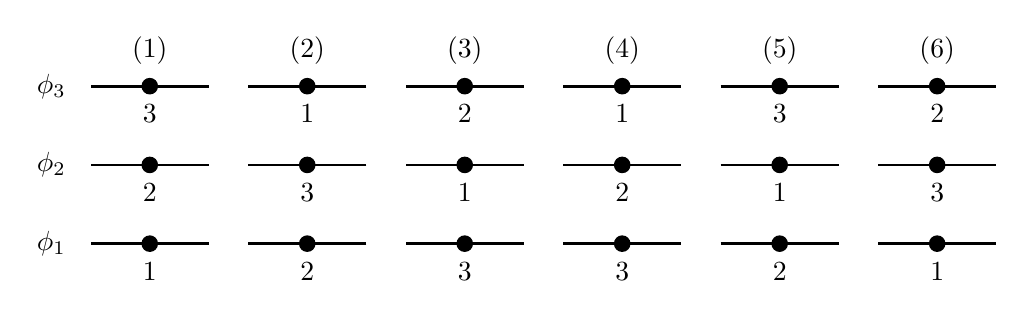
\begin{tikzpicture}
		\node at (-6.25, 2) {$\phi_3$};
		\node at (-6.25, 1) {$\phi_2$};
		\node at (-6.25, 0) {$\phi_1$};

		\node at (-5, 2.45) {(1)};
		\draw[line width=1pt] (-4.25, 2) -- (-5.75, 2);
		\draw[line width=1pt] (-4.25, 1) -- (-5.75, 1);
		\draw[line width=1pt] (-4.25, 0) -- (-5.75, 0);
		\fill (-5, 0)circle(3pt) (-5, 1)circle(3pt) (-5, 2)circle(3pt);
		\node at (-5, -0.35) {$1$};
		\node at (-5,  0.65) {$2$};
		\node at (-5,  1.65) {$3$};

		\node at (-3, 2.45) {(2)};
		\draw[line width=1pt] (-2.25, 2) -- (-3.75, 2);
		\draw[line width=1pt] (-2.25, 1) -- (-3.75, 1);
		\draw[line width=1pt] (-2.25, 0) -- (-3.75, 0);
		\fill (-3, 0)circle(3pt) (-3, 1)circle(3pt) (-3, 2)circle(3pt);
		\node at (-3, -0.35) {$2$};
		\node at (-3,  0.65) {$3$};
		\node at (-3,  1.65) {$1$};

		\node at (-1, 2.45) {(3)};
		\draw[line width=1pt] (-0.25, 2) -- (-1.75, 2);
		\draw[line width=1pt] (-0.25, 1) -- (-1.75, 1);
		\draw[line width=1pt] (-0.25, 0) -- (-1.75, 0);
		\fill (-1, 0)circle(3pt) (-1, 1)circle(3pt) (-1, 2)circle(3pt);
		\node at (-1, -0.35) {$3$};
		\node at (-1,  0.65) {$1$};
		\node at (-1,  1.65) {$2$};

		\node at (1, 2.45) {(4)};
		\draw[line width=1pt] (0.25, 2) -- (1.75, 2);
		\draw[line width=1pt] (0.25, 1) -- (1.75, 1);
		\draw[line width=1pt] (0.25, 0) -- (1.75, 0);
		\fill (1, 0)circle(3pt) (1, 1)circle(3pt) (1, 2)circle(3pt);
		\node at (1, -0.35) {$3$};
		\node at (1,  0.65) {$2$};
		\node at (1,  1.65) {$1$};

		\node at (3, 2.45) {(5)};
		\draw[line width=1pt] (2.25, 2) -- (3.75, 2);
		\draw[line width=1pt] (2.25, 1) -- (3.75, 1);
		\draw[line width=1pt] (2.25, 0) -- (3.75, 0);
		\fill (3, 0)circle(3pt) (3, 1)circle(3pt) (3, 2)circle(3pt);
		\node at (3, -0.35) {$2$};
		\node at (3,  0.65) {$1$};
		\node at (3,  1.65) {$3$};

		\node at (5, 2.45) {(6)};
		\draw[line width=1pt] (4.25, 2) -- (5.75, 2);
		\draw[line width=1pt] (4.25, 1) -- (5.75, 1);
		\draw[line width=1pt] (4.25, 0) -- (5.75, 0);
		\fill (5, 0)circle(3pt) (5, 1)circle(3pt) (5, 2)circle(3pt);
		\node at (5, -0.35) {$1$};
		\node at (5,  0.65) {$3$};
		\node at (5,  1.65) {$2$};
	\end{tikzpicture}	
	\caption{三粒子填充三条能级的体系集体波函数情况}
	\label{fig:three-body-wv}
\end{figure}

\paragraph*{平均场的迭代求解:}
平均场下的\textsl{Hartree(-Fock)}方程如下:
\begin{equation}
    \begin{aligned}
        \frac{-\hbar^{2}}{2m_N} \nabla^{2} \phi_{\alpha}(\bm{r}) + V_{H(F)}\left(
        \{\phi_{i}(\bm{r})\}\right) = \varepsilon_{\alpha}\phi_{\alpha}(\bm{r}) \\ 
        i = 1, 2, \cdots, A, \quad \alpha = 1, 2, \cdots, \infty
    \end{aligned}
    \label{eq:Hartree-Fock}
\end{equation}
上式与薛定谔方程唯一不同就是势能变成了关于波函数的非线性函数,
\begin{equation*} V(\bm{r}) \Longrightarrow V_{H(F)}(\{\phi_{i}(\bm{r})\})
\end{equation*}
式\eqref{eq:Hartree-Fock}为非线性方程组,一般用迭代的方法求解。我们先猜测得到一组试探
波函数${\phi_i^0(\bm{r})}_{i=1}^{A}$,然后我们根据势能与波函数的关系得到初始势场
$V_{H(F)}^{0}$;完成上述步骤后,我们将试探波函数和初始势场带入式\eqref{eq:Hartree-Fock},
求解得到一组新的波函数${\phi_{\alpha}^0(\bm{r})}_{\alpha=1}^{A}$和本征值$\varepsilon_{\alpha}^{(1)}$,
通过这组新的波函数,我们可以再次生成一个新的势场$V_{H(F)}^{(1)}$;将生成的新势场和新波函数
再次代入式\eqref{eq:Hartree-Fock},可得到更新一组的本征波函数和本征能量。通过比较某次迭代
前后的波函数间的误差小于某一给定值来确定波函数合理
\begin{equation}
    \parallel \phi_{\alpha}^{(n-1)} - \phi_{\alpha}^{(n)} \parallel < \text{preset limit}
    \label{eq:iter-error}
\end{equation}
其中,$\parallel \cdots \parallel$表示波函数的模。

\uline{关于平均势场和初始波函数形式的选取}:上述平均场方程中,势能具体形式为
\begin{equation}
    V_{H(F)}\left( \left\{ \phi_i(\bm{r}) \right\} \right) = \sum_{i \neq j} \int 
    \phi_i^{\star}(\bm{r}_i^{\prime}) V_{ij}(\bm{r}_i^{\prime}, \bm{r}_j) \phi_{i}(\bm{r}_i^{\prime})
    \,d\bm{r}_i^{\prime}
    \label{eq:mean-field}
\end{equation}
为寻找到一组合适的平均场,试探波函数可以选取一组零级近似,如费米气体模型单粒子波函数:
\begin{equation}
    \phi_i = \sqrt{V^{-1}} \exp{(i \bm{k}_i \cdot \bm{r}_i)}
    \label{eq:fermi-gas-eigen}
\end{equation}
其中,$V$表示原子核的体积。对于二体势$V_{ij}$,可以选用Skyrme力(见下式)或其它形式的两体力
\begin{equation}
    V_{skyrme} = \sum_{i<j} v(i, j) + \sum_{i<j<k} v(i, j, k)
    \label{eq:skyrme-forc}
\end{equation}
其中,两体力部分为
\begin{equation}
    \begin{aligned}
        v(1, 2) =& t_0 (1 + x_0 P_{\sigma})\delta(\bm{r}_1 - \bm{r}_2) \\
            & + t_1\left[ \delta(\bm{r}_1 - \bm{r}_2) \bm{k}^{2}
              + \bm{k}^{\prime 2}\delta(\bm{r}_1 - \bm{r}_2)\right] / 2 \\
            & + t_2\bm{k}^{\prime} \cdot \delta(\bm{r}_1 - \bm{r}_2) \bm{k} \\
            & + {\rm i} W_0(\bm{\sigma}_1 + \bm{\sigma}_2)\cdot \left[ 
            \bm{k}^{\prime} \times \delta\left( \bm{r}_1 - \bm{r}_2 \right) \bm{k}\right]
    \end{aligned}
    \label{eq:skyrme-tow-body-forc}
\end{equation}
三体部分为
\begin{equation}
    v(1, 2, 3) = t_3 \delta(\bm{r}_1 - \bm{r}_2) \delta(\bm{r}_2 - \bm{r}_3)
    \label{eq:skyrm-three-body-forc}
\end{equation}
式中,$\bm{k} = \bm{p}/\hbar = (\nabla_{1} - \nabla_{2}) / (2{\rm i})$是向右作用的相对动量
算符,$\bm{k}^{\prime} = \bm{p}/\hbar = (\nabla_{2} - \nabla_{1}) / (2{\rm i})$是向左相对
动量算符;$P_{\sigma} = (1 + \bm{\sigma}_1 \cdot \bm{\sigma}_2) / 2$是自旋交换算符。上式
Skyrme力有6个可调参数$t_0$、$t_1$、$t_2$、$t_3$、$x_0$和$W_0$。

\paragraph*{唯象势}

\section{Woods-Saxon波函数用球谐振子基展开}
\subsection{径向方程}
单核子薛定谔方程中的哈密顿量为:
\begin{equation}
	\begin{aligned}
		h =& \frac{-\hbar^2}{2 m_{N}} \nabla^2 + v(r) + v_{LS}(r) \boldsymbol{L\cdot S}	\\
		=& \frac{-\hbar^2}{2 m_{N}}\left(\nabla^2_{r} - \frac{\boldsymbol{L}/\hbar^2}{r^2} + v_{WS}(r) + v_{C}(r) + v_{LS}(r)\boldsymbol{L\cdot S}\right)
	\end{aligned}
\end{equation} 
其中,径向偏分取一般形式
\begin{equation}
	\nabla^2_{r} \equiv \frac{1}{r^2} \frac{d}{dr} \left(r^2 \frac{d}{dr}\right)
\end{equation}
$v_{WS}$是Woods-Saxon势,$v_{C}(r)$为库伦势,原子核半径内取均匀带电的球静态库伦势,可得方程如下
\begin{equation}
	v_{C} = \frac{Ze^2}{4\pi\epsilon_0}
\end{equation} 

\subsection{Woods-Saxon哈密顿量的对角化}
得到球谐振子波函数后,可将这些波函数作为基矢展开构成Woods-Saxon势下的原子核波函数。谐振子展开的Woods-Saxon径向哈密顿量矩阵元为
\begin{equation}
    \begin{aligned}
		\langle \nu^{\prime} | h_{lj}(r) | \nu\rangle =&\int_{0}^{\infty} r^2 \,dr g_{\nu^{\prime} l}(r) g_{\nu l}(r) \left[ \frac{\hbar^2}{2m_N} \left(\frac{4n + 2l + 3}{b^2} - \frac{r^2}{b^4}\right) \right. \\
		&+ \left. v_{WS}(r) + v_{C}(r) + \frac{1}{2}\left[j(j+1) - l(l+1) - \frac{3}{4}\hbar^2 v_{LS}(r)\right] \right]
    \end{aligned}
\end{equation}
这样,整个矩阵就可以写成如下形式
\begin{equation}
	\begin{bmatrix}
		\langle 0 | h_{lj}(r) | 0 \rangle & \langle 0 | h_{lj}(r) | 1 \rangle & \cdots	& \cdots	\\
		\langle 1 | h_{lj}(r) | 0 \rangle & \langle 1 | h_{lj}(r) | 1 \rangle & \cdots	& \cdots	\\
		\vdots	&	\vdots	& \ddots
	\end{bmatrix}
\end{equation}
这样,当我们对角化该矩阵后就可以知道此径向哈密顿量在谐振子基上的能量,通过比例关系就可以知道对应谐振子基上的系数$A_{\nu}^{(nlj)}$。



\chapter{占据数表象}

\section{多粒子态表象}
\paragraph*{$N$粒子系统的基矢:}以某一中原子核组态$|\alpha_1\ \alpha_2 \cdots \alpha_N\rangle$

%%%%%%%%%%%%%%%%%%%%%%%%%%%%%%%%%%%%%%%%%%%%%%%%
\part{科研笔记}
\chapter{The Time-Dependent Hartree-Fock Method(TDHF)}

\begin{introduction}
  \item A detailed derivation about TDHF
\end{introduction}
  $\ast -- $ \textcolor{purple}{\textit{The Nuclear Many-Body Problem}}

  \section{Time-Denpendent Hartree-Fock Method}
  The processes in nuclei involving large amplititudes(anharmonic vibrations, fission and fussion processes) can be formulated in a time-dependent way.  \textcolor{blue}{*In a microscopic picture, such a deformed state would be represented by a Slater determinant in a deformed potential well, which is certainly no eigenstate of $H$, but a wave packet in the sense of Eq.\eqref{tdhf1}}.

  Let's start with an arbitrary wave packet $\mid\Psi(0)\rangle$, its exact time evolution is:
  \begin{equation}
    \Psi(t) = e^{-iHt/\hbar}\mid \Psi(0)\rangle \label{tdhf1} 
  \end{equation}
  and its one-body density at time $t$ is given by
  \begin{equation}
    \rho_{kl}(t) = \langle \Psi(t) \mid c_l^\dagger c_k \mid \Psi(t) \rangle  \label{tdhf2}
  \end{equation}
  In order to obtain equation of motion, we calculate its time derivative:
  \begin{equation}
    i\hbar\dot{\rho}_{kl}(t) = \langle \Psi(t) | [c_l^\dagger c_k, H] | \Psi(t) \rangle \label{tdhf3}
  \end{equation}

  \begin{proof}
    we use the Sch{\"o}dinger equation, and we calculate it in Sch{\"o}dinger picture that the operator don't evaluate with time.
    \begin{equation}
      \begin{aligned}
        \dot{\rho}_{kl}(t) =& \frac{d}{dt}\rho_{kl}(t) = \frac{d}{dt}\left[\langle \Psi(t) \mid c_l^\dagger c_k \mid \Psi(t) \rangle\right]\\
                                =& \left( \frac{d}{dt}(\langle \Psi(t) \mid) c_l^\dagger c_k \mid \Psi(t) \rangle + \langle \Psi(t) \mid \frac{d}{dt}(c_l^\dagger c_k) \mid \Psi(t) \rangle + \langle \Psi(t) \mid c_l^\dagger c_k \frac{d}{dt}(\mid \Psi(t) \rangle)\right)\\
                                =& -\frac{1}{i\hbar}\langle \Psi(t) \mid Hc_l^\dagger c_k \mid \Psi(t) \rangle + \frac{1}{i\hbar}\langle \Psi(t) \mid c_l^\dagger c_kH \mid \Psi(t) \rangle\\
                                =&\frac{1}{i\hbar}\langle \Psi(t) \mid [c_l^\dagger c_k,H] \mid \Psi(t) \rangle \label{tdhf4}
      \end{aligned}
    \end{equation}
  \end{proof}

  In HF theory, the Hamiltonian is
  \begin{equation}
    H = \sum_{pr}t_{pr} c_p^\dagger c_r + \frac{1}{4}\sum_{prsj}\bar{v}_{prsj}c_p^\dagger c_r^\dagger c_j c_s \label{tdhf5}
  \end{equation}
  according the equation above, the two-body Hamiltonian can be written as
  \begin{equation}
    i\hbar\dot{\rho}_{kl} - \sum_{p}(t_{kp}\rho_{pl}-\rho_{kp}t_{pl}) = \frac{1}{2}\sum_{prs} \left(\bar{v}_{kprs}\rho_{rslp}^{(2)} - \bar{v}_{rslp}\rho_{kprs}^{2}\right) \label{tdhf6}
  \end{equation}
  where we have introduced the two-body density
  \begin{equation}
    \rho_{klpq}^{(2)}(t) = \langle \Psi(t) | c_p^\dagger c_q^\dagger c_l c_k | \Psi(t) \rangle  \label{tdhf7}
  \end{equation}
  \begin{proof}
    According to Eq.\eqref{tdhf3} and Eq.\eqref{tdhf3}  the firs term of l.h.s in Eq.\eqref{tdhf5} equals to
    \begin{equation}
      \begin{aligned}
        i\hbar\dot{\rho}_{kl}(t) =& \langle \Psi(t) | [c_l^\dagger c_k, H] | \Psi(t) \rangle \\
                                 =& \left\langle \Psi(t) \left| \sum_{pr}t_{pr}[c_l^\dagger c_k, c_p^\dagger c_r] + \frac{1}{4}\sum_{prsj}\bar{v}_{prsj}[c_l^\dagger c_k, c_p^\dagger c_r^\dagger c_jc_s] \right| \Psi(t) \right\rangle  \label{tdhf8}
      \end{aligned}
    \end{equation}

    $\bullet$ (1)We first calculate the term $\sum\limits_{pr}t_{pr}[c_l^\dagger c_k, c_p^\dagger c_r]$, note that we calculate the equation under a Fermion system, so we have the equation:
    \begin{equation}
      \{a_\alpha, a_\beta^\dagger\} = \delta_{\alpha\beta}, \quad  \{a_\alpha^\dagger, a_\beta^\dagger\} = \{a_\alpha, a_\beta\} = 0 \label{tdhf9}
    \end{equation}
    and in addition, for commutation relations we have the  equation
    \begin{equation}
      [\hat{A}\hat{B}, \hat{C}] = \hat{A}\{\hat{B}, \hat{C}\} - \{\hat{A}, \hat{C}\}\hat{B} \label{tdhf10}
    \end{equation}
    therefore, we have
    \begin{equation}
      \begin{aligned}
      \sum_{pr}t_{pr}\left([c_l^\dagger c_k, c_p^\dagger c_r]\right) =& \sum_{pr}t_{pr}\left(c_p^\dagger [c_l^\dagger c_k,c_r] + [c_l^\dagger c_k,c_p^\dagger ]c_r\right)\\
                        =& \sum_{pr}t_{pr}\left(c_p^\dagger \left( c_l^\dagger \cancel{\{{c_k, c_r}\}} - \{{c_l^\dagger, c_r}\}c_k \right) + \left( c_l^\dagger\{c_k, c_p^\dagger\} - \cancel{\{c_l^\dagger, c_p^\dagger\}}c_k \right)c_r\right)\\
                        =& \sum_{pr}t_{pr}\left(-c_p^\dagger \{{c_l^\dagger, c_r}c_k\} + c_l^\dagger\{c_k, c_p^\dagger\}c_r\right)\\
                        =& \sum_{pr}t_{pr}\left(-\delta_{lr}c_p^\dagger c_k + \delta_{kp}c_l^\dagger c_r\right) \label{tdhf11}
      \end{aligned}
    \end{equation}
    consider four cases
    \begin{itemize}
      \item $k\neq p, l \neq r$ \[\sum_{pr}t_{pr}\left(-\delta_{lr}c_p^\dagger c_k + \delta_{kp}c_l^\dagger c_r\right)=0\]
      \item $k\neq p, l = r$  \[\sum_{pr}t_{pr}\left(-\delta_{lr}c_p^\dagger c_k + \delta_{kp}c_l^\dagger c_r\right)=\sum_{pr}-t_{pl}c_p^\dagger c_k\]
      \item $k = p, l \neq r$ \[\sum_{pr}t_{pr}\left(-\delta_{lr}c_p^\dagger c_k + \delta_{kp}c_l^\dagger c_r\right)=\sum_{r}-t_{kr}c_l^\dagger c_r\]
            use the dummy index $p$ replace $r$ and has
            \[\sum_{pr}t_{pr}\left(-\delta_{lr}c_p^\dagger c_k + \delta_{kp}c_l^\dagger c_r\right)=\sum_{p}-t_{kp}c_l^\dagger c_p\]
      \item $k = p, l \neq r$ \[ \sum_{pr}t_{pr}\left(-\delta_{lr}c_p^\dagger c_k + \delta_{kp}c_l^\dagger c_r\right) = c_l^\dagger c_l - c_p^\dagger c_p\]
    \end{itemize}
    according to the case above, we finally has the form
    \begin{equation}
      \sum_{pr}t_{pr}\left([c_l^\dagger c_k, c_p^\dagger c_r]\right) = \sum_{p}(t_{kp}c_l^\dagger c_p-t_{pl}c_p^\dagger c_k) \label{tdhf12}
    \end{equation}

    $\bullet$ (2)Then we calculate the formulation $\sum\limits_{prsj} \bar{v}_{p r s j}\left[c_{l}^{\dagger} c_{k}, c_{p}^{\dagger} c_{r}^{\dagger} c_{j} c_{s}\right]$, we have
    \begin{equation}
      \begin{aligned}
        \left[c_{l}^{\dagger} c_{k}, c_{p}^{\dagger} c_{r}^{\dagger} c_{j} c_{s}\right] =& c_{p}^{\dagger} c_{r}^{\dagger} c_{j}[c_{l}^{\dagger} c_{k}, c_{s}] + [c_{l}^{\dagger} c_{k},c_{p}^{\dagger} c_{r}^{\dagger} c_{j} ]c_{s}\\
        =&c_{p}^{\dagger} c_{r}^{\dagger} c_{j}[c_{l}^{\dagger} c_{k}, c_{s}]+ (c_{p}^{\dagger} c_{r}^{\dagger}[c_{l}^{\dagger} c_{k},c_{j} ]+[c_{l}^{\dagger} c_{k},c_{p}^{\dagger} c_{r}^{\dagger}  ]c_{j})c_{s}\\
        =&c_{p}^{\dagger} c_{r}^{\dagger} c_{j}[c_{l}^{\dagger} c_{k}, c_{s}]+ c_{p}^{\dagger} c_{r}^{\dagger}[c_{l}^{\dagger} c_{k},c_{j} ]c_{s}+[c_{l}^{\dagger} c_{k},c_{p}^{\dagger} c_{r}^{\dagger}]c_{j}c_{s}\\
        =&c_{p}^{\dagger} c_{r}^{\dagger} c_{j}[c_{l}^{\dagger} c_{k}, c_{s}]+ c_{p}^{\dagger} c_{r}^{\dagger}[c_{l}^{\dagger} c_{k},c_{j} ]c_{s}\\
         &+(c_{p}^{\dagger}[ c_{l}^{\dagger} c_{k}, c_{r}^{\dagger} ] + [ c_{l}^{\dagger} c_{k},c_{p}^{\dagger} ]c_{r}^{\dagger})c_{j}c_{s}\\
        =&c_{p}^{\dagger} c_{r}^{\dagger} c_{j}[c_{l}^{\dagger} c_{k}, c_{s}]+ c_{p}^{\dagger} c_{r}^{\dagger}[c_{l}^{\dagger} c_{k},c_{j} ]c_{s}\\
         &+c_{p}^{\dagger}[ c_{l}^{\dagger} c_{k}, c_{r}^{\dagger} ]c_j c_{s} + [ c_{l}^{\dagger} c_{k},c_{p}^{\dagger} ]c_{r}^{\dagger})c_{j}c_{s}\\
        =&c_{p}^{\dagger} c_{r}^{\dagger} c_{j}(c_{l}^{\dagger} \cancel{\{c_{k}, c_{s}]\}} - \{c_{l}^{\dagger}, c_{s}]\}c_{k})+ c_{p}^{\dagger} c_{r}^{\dagger}(c_{l}^{\dagger} \cancel{\{c_{k}, c_{j}]\}} - \{c_{l}^{\dagger}, c_{j}]\}c_{k})c_{s}\\
        &+c_{p}^{\dagger}(c_{l}^{\dagger} \cancel{\{c_{k}, c_{r}]\}} - \{c_{l}^{\dagger}, c_{r}]\}c_{k})c_{j}c_{s} + (c_{l}^{\dagger}\{c_{k}, c_{p}^\dagger]\} - \cancel{\{c_{l}^{\dagger}, c_{p}^\dagger\}}c_{k})c_{r}^{\dagger}c_{j}c_{s}\\
        =&-\delta_{ls}c_p^\dagger c_r^\dagger c_j c_k -\delta_{lj}c_p^\dagger c_r^\dagger c_k c_s + \delta_{kr}c_p^\dagger c_l^\dagger c_j c_s + \delta_{kp}c_l^\dagger c_r^\dagger c_j c_s \label{tdhf13}
      \end{aligned}
    \end{equation}
    so we get
    \begin{equation}
      \begin{aligned}
         & \sum_{prsj}\bar{v}_{prsj}[c_{l}^{\dagger} c_{k}, c_{p}^{\dagger} c_{r}^{\dagger} c_{j} c_{s}]\\
        =& \sum_{prsj}\bar{v}_{prsj}(-\delta_{ls}c_p^\dagger c_r^\dagger c_j c_k -\delta_{lj}c_p^\dagger c_r^\dagger c_k c_s + \delta_{kr}c_p^\dagger c_l^\dagger c_j c_s + \delta_{kp}c_l^\dagger c_r^\dagger c_j c_s)\\
        =& \sum_{prsj}\bar{v}_{prsj}(\delta_{kp}c_l^\dagger c_r^\dagger c_j c_s + \delta_{kr}c_p^\dagger c_l^\dagger c_j c_s - \delta_{ls}c_p^\dagger c_r^\dagger c_j c_k -\delta_{lj}c_p^\dagger c_r^\dagger c_k c_s)\\
        =& \sum_{rsj}\bar{v}_{krsj}c_l^\dagger c_r^\dagger c_j c_s + \sum_{psj}\bar{v}_{pksj}c_p^\dagger c_l^\dagger c_j c_s - \sum_{prj}\bar{v}_{prlj}c_p^\dagger c_r^\dagger c_j c_k - \sum_{prs}\bar{v}_{prsl}c_p^\dagger c_r^\dagger c_k c_s\\
        =& \sum_{prs}\bar{v}_{kprs}c_l^\dagger c_p^\dagger c_s c_r + \sum_{psr}\bar{v}_{pksr}c_p^\dagger c_l^\dagger c_r c_s - \sum_{prs}\bar{v}_{rslp}c_r^\dagger c_s^\dagger c_p c_k - \sum_{prs}\bar{v}_{rspl}c_r^\dagger c_s^\dagger c_k c_p\\ 
        =& \sum_{prs}\bar{v}_{kprs}c_l^\dagger c_p^\dagger c_s c_r + \sum_{prs}\bar{v}_{kprs}c_l^\dagger c_p^\dagger c_s c_r - \sum_{prs}\bar{v}_{rslp}c_r^\dagger c_s^\dagger c_p c_k - \sum_{prs}\bar{v}_{rslp}c_r^\dagger c_s^\dagger c_p c_k\\
        =& 2\sum_{prs}\bar{v}_{kprs}c_l^\dagger c_p^\dagger c_s c_r - 2\sum_{prs}\bar{v}_{rslp}c_r^\dagger c_s^\dagger c_p c_k\\ \label{tdhf14}
      \end{aligned}
    \end{equation}
    in the fifth equation we use the property
    \begin{equation}
      \bar{v}_{prsl} = -\bar{v}_{prls} = -\bar{v}_{rpsl} = \bar{v}_{rpsl} \label{tdhf15}
    \end{equation}
    Insert Eq.\eqref{tdhf12}, \eqref{tdhf14} and \eqref{tdhf8} into l.h.s of Eq.\eqref{tdhf6}, and then get the r.h.s.
  \end{proof}

  The l.h.s of Eq.\eqref{tdhf6} describes the free motion of the system, it contains only the kinetic energy. And the r.h.s of Eq.\eqref{tdhf6} contains the interaction between the particles. This interaction can be divided into two parts --- a self-consistent one-body field, which averages over all particles, and individual collisions between two nucleons which cannot be taken into account by the mean field. The latter causes the two-body correlations.

  To achieve this decomposition we define a correlation function $g^{(2)}$ by extracting the uncorrelated pairs of $\rho^{(2)}$,
  \begin{equation}
    \rho_{klpq}^{(2)}(t) = \rho_{kp}\rho_{lq} - \rho_{kq}\rho_{lp} + g_{rslp}^{(2)} \label{tdhf16}
  \end{equation}
  and gain, instead of Eq.\eqref{tdhf6}
  \begin{equation}
    i\hbar\dot{\rho}_{kl} - [t+\Gamma, \rho]_{kl} = \frac{1}{2}\sum_{prs} \left(\bar{v}_{kprs}g_{rslp}^{(2)} - \bar{v}_{rslp}g_{kprs}^{(2)}\right) \label{tdhf17}
  \end{equation}
  with the density dependent HF potentia
  \begin{equation}
    \Gamma_{kl} = \sum_{pq}\bar{v}_{kqlp}\rho_{pq}  \label{tdhf18}
  \end{equation}

  \begin{note}
    The self-consistent field $\Gamma$ is time dependent. And for an element of the product of two matrices $t$ and $\rho$ can be written as
    \begin{equation}
      [t\rho]_{kl} = \sum_{p}t_{kp}\rho_{pl}  \label{tdhf19}
    \end{equation}
    We used Wick's theorem in Eq.\eqref{tdhf16}, and the term $g_{rslp}^{(2)}$ contains the residual interaction force( just like pairing force).
  \end{note}

  Particles in this system can now undergo two kinds of interactions --- collisons with the moving walls of the self-consistent field $\Gamma$ or collisions with the other particles. Both types provide internal excitations of the system. We expect that two-body scattering plays no essential role in the dynamical case, as long as the excitation energies per particle are less than the Fermi energy and $g^{(2)}$ may be neglected. 
  
  For $g^{(2)}=0$ we therefore end up with the \textit{TDHF equation}
  \begin{equation}
    i\hbar\dot{\rho} = [h,\rho] \label{tdhf20}
  \end{equation} 


%%%%%%%%%%%%%%%%%%%%%%%%%%%%%%%%%%%%%%%%%%%%%%%%%%%%%%%%
  \section{Adiabatic Time-Dependent Hartree-Fock Method}

  The theory involves \textcolor{red}{two approximations:} \newline
  \textcolor{red}{1}.The \textit{TDHF assumption}, where the wave functions stay a Slater determinant at all times;\newline
  \textcolor{red}{2}.The \textit{adabatic approach}, where we must include the velocities only to second order.

  In ATDHF, the motion of collective system is much slower than the motion of nucleon.
  \vspace{8pt}

  TIn TDHF theory everything is determined by the single-particle density $\rho(t)$, which is not time-reversal invariant. Since we want to have time-reversal invariant coordinates, Baranger and Veneroni proposed the following decomposition of the density $\rho(t)$
  \begin{equation}
    \rho(t) = e^{(i/\hbar)\chi(t)}\rho_0(t)e^{-(i/\hbar)\chi(t)} \label{tdhf21}
  \end{equation}
  where $\rho_0$ and $\chi$ are both \textcolor{blue}{Hermitian, time-even matrices}. And $\rho_0$ satisfies
  \begin{equation}
    \rho_0^2 = \rho_0, \quad {\rm Tr}\rho_0 = N \label{tdhf22}
  \end{equation}
  it corresponds to an $N$-dimensional Slater determinant $|\Psi_0\rangle$. In the following the $\rho_0$ shall be the \textcolor{blue}{coordinate} and $\chi$ shall be the \textcolor{blue}{momentum}.

  Eq.\eqref{tdhf21} is unique under the following conditions:
  \begin{itemize}
    \item [(i)] $\chi$ has only eigenvalues $\chi_\mu$ with
                \begin{equation}
                  -\frac{\pi}{4}\hbar \leqslant \chi_\mu < \frac{\pi}{4}\hbar \label{tdhf23}
                \end{equation}
    \item[(ii)] The $pp$ and $hh$ matrix elements of $\chi$ vanish in the basis in which $\rho_0$ is diagonal, that is 
                \begin{equation}
                  \chi^{hh}=\rho_0\chi\rho_0=0, \quad \chi^{pp} = \sigma_0\chi\sigma_0=0  \label{tdhf24}
                \end{equation}
  \end{itemize}
  \begin{note}
    $\rho_0$ is the projector onto hole state and $\sigma_0=1-\rho_0$ is the projector onto particle states in the basis in which $\rho_0$ is diagonal.
  \end{note}

  The \textit{adiabatic approximation} consists in assuming that the density $\rho(t)$ of the system is at all times close to the density $\rho_0(t)$, and the density $\rho_0(t)$ don't evaluated with time, so it means that \textcolor{blue}{we have a nearly static density at all times}. In other words, \textcolor{blue}{it means that the matrix $\chi$ which introduce time-odd components is small.}

  Expand $\rho(t)$ up to second order in $\chi$ and get
  \begin{equation}
    \rho=e^{(i/\hbar)\chi(t)}\rho_{0}e^{-(i/\hbar)\chi(t)} \simeq \rho_0 + \rho_1 + \rho_2  \label{tdhf25}
  \end{equation}
  with 
  \begin{equation}
    \rho_1 = \frac{i}{\hbar}[\chi, \rho_0], \quad \chi=-i\hbar[\rho_1,\rho_0] \label{tdhf26}
  \end{equation}
  \begin{equation}
    \rho_2=\frac{-1}{2\hbar^2} [ \chi,\left[ \chi,\rho_0] \right] = \frac{1}{\hbar^2}\left( \chi\rho_0\chi - \frac{1}{2}(\chi^2\rho_0+\rho_0\chi^2) \right) \label{tdhf27}
  \end{equation}
  \begin{proof}
    Implement the Taylor Expantion of $\rho$ and only preserve to second order term
    \begin{equation}
      \begin{aligned}
        \rho =& e^{(i/\hbar)\chi(t)}\rho_{0}e^{-(i/\hbar)\chi(t)}\\                                       \label{tdhf28}  
             \simeq & \left[ 1 + \frac{i\chi}{\hbar} - \frac{1}{2}\left(\frac{\chi}{\hbar}\right)^2 \right] \rho_0 \left[ 1 - \frac{i\chi}{\hbar} - \frac{1}{2}\left(\frac{\chi}{\hbar}\right)^2 \right] \\
             =& \left[1+\frac{i}{\hbar}\chi - \frac{1}{2\hbar}^2\chi^2 \right] \left[ \rho_0 - \frac{i}{\hbar}\rho_0\chi - \frac{1}{2\hbar}^2\rho_0\chi^2 \right] \\
             =& \rho_0 - \frac{i}{\hbar}\rho_0\chi \ \frac{1}{2\hbar^2}\rho_0\chi^2 + \frac{i}{\hbar}\chi\rho_0 + \frac{1}{\hbar^2}\chi\rho_0\chi - \cancel{\frac{i}{\hbar^3}\chi\rho_0\chi^2}\\
              &  - \frac{1}{2\hbar^2}\chi^2\rho_0 + \cancel{\frac{i}{2\hbar^3}\chi^2\rho_0\chi} + \cancel{\frac{1}{4\hbar^4}\chi^2\rho_0\chi^2}\\
             =& \rho_0 + \frac{i}{\hbar}(\chi\rho_0 - \rho_0\chi) + \frac{1}{\hbar^2}[\chi\rho_0\chi - \frac{1}{2}(\chi^2\rho_0 + \rho_0\chi^2)] \\
             =& \rho_0 + \frac{i}{\hbar}[\chi, \rho_0] + \frac{1}{2\hbar^2}[\chi\rho_0\chi - \chi^2\rho_0 + \chi\rho_0\chi - \rho_0\chi^2]\\
             =& \rho_0 + \frac{i}{\hbar}[\chi, \rho_0] + \frac{1}{2\hbar^2}[\chi(\rho_0\chi - \chi\rho_0) + (\chi\rho_0 - \rho_0\chi)\chi]\\
             =& \rho_0 + \frac{i}{\hbar}[\chi, \rho_0] + \frac{1}{2\hbar^2}[\chi(\rho_0\chi - \chi\rho_0) - (\rho_0\chi - \chi\rho_0)\chi]\\
             =& \rho_0 + \frac{i}{\hbar}[\chi, \rho_0] + \frac{1}{2\hbar^2}[\chi, [\rho_0,\chi]]\\
             =& \rho_0 + \frac{i}{\hbar}[\chi, \rho_0] - \frac{1}{2\hbar^2}[\chi, [\chi,\rho_0]]\\          
             =& \rho_0 + \rho_1 + \rho_2\\                                                                      
      \end{aligned}
    \end{equation}
    where we define
    \begin{equation}
      \rho_1 = \frac{i}{\hbar}[\chi, \rho_0], \quad \rho_2=\frac{-1}{2\hbar^2} [ \chi,\left[ \chi,\rho_0] \right] \label{tdhf29}
    \end{equation}
    According to Eq.\eqref{tdhf24}, we have
    \begin{equation}
      \begin{aligned}
        \sigma_0\chi\sigma_0 =& (1-\rho_0)\chi(1-\rho_0) = (1-\rho_0)(\chi-\chi\rho_0)\\      \label{tdhf30}
                             =& \chi - \chi\rho_0 - \rho_0\chi + \cancel{\rho_0\chi\rho_0}\\
                             =& \chi - \chi\rho_0 - \rho_0\chi \\
                             =& 0                                       
      \end{aligned}
    \end{equation}
    so, we get
    \begin{equation}
      \chi = \chi\rho_0 + \rho_0\chi    \label{tdhf31}
    \end{equation}
    and according to Eq.\eqref{tdhf29}, we have
    \begin{equation}
      i\hbar\rho_1 = \rho_0\chi - \chi\rho_0    \label{tdhf32}
    \end{equation}
    therefore, we get
    \begin{subequations}
      \begin{align}
        i\hbar\rho_1\rho_0 =& \rho_0\chi\rho_0 - \chi\rho_0^2 =  \rho_0\chi\rho_0 - \chi\rho_0 = - \chi\rho_0     \label{tdhf33a}\\
        i\hbar\rho_0\rho_1 =& \rho_0^2\chi - \rho_0\chi\rho_0 =  \rho_0\chi - \rho_0\chi\rho_0 = \rho_0\chi       \label{tdhf33b}
      \end{align}
    \end{subequations}
    Eq.\eqref{tdhf33b} - Eq.\eqref{tdhf33a}, and get
    \begin{equation}
      \begin{aligned}
        i\hbar(\rho_0\rho_1 - \rho_1\rho_0) = -i\hbar(\rho_1\rho_0 - \rho_0\rho_1) = -i\hbar[\rho_1, \rho_0] = \rho_0\chi + \chi\rho_0 = \chi   \label{tdhf34}
      \end{aligned}
    \end{equation}
  \end{proof}
  
  We can proove that $\rho_1$ has only $ph-$ and $hp-$ and that $\rho_2$ has only $pp-$ and $hh-$matrix elements:
  \begin{align}
    \label{tdhf35} \rho_1 =& \frac{i}{\hbar}(\sigma_0\chi\rho_0-\rho_0\chi\sigma_0)\\        
    \label{tdhf36} \rho_2 =& \sigma_0\rho_1^2\sigma_0 - \rho_0\rho_1^2\rho_0                 
  \end{align}
  \begin{note}
    In order to proove these two equation, we need to define the following rules for calculating with single-particle densities $\rho$ of Slater determinans$(\rho^2=\rho, \sigma=1-\rho)$\textcolor{purple}{(see D.31, D.32, Appedinx D, The Nuclear Many-Body Problem)}.

    An arbitrary matrix $A$ has the folloing $pp$, $ph$, $hp$ and $hh$ parts in a basis in which $\rho$ is diagonal:
    \begin{equation}
      A^{pp}:= \sigma A \sigma; \quad  A^{hh}:= \rho A \rho; \quad A^{ph}=\sigma A \rho; \quad A^{hp}=\rho A \sigma \label{tdhf37}
    \end{equation}
    The three statements
    \begin{equation}
      A = A\rho + \rho A \Leftrightarrow A = A\sigma + \sigma A \Leftrightarrow A^{pp}=A^{hh}=0 \label{tdhf38}
    \end{equation}
    are equivalent. 
    
    If two matrices $A$ and $B$ obey the relation $B=[A,\rho]$, it follows:
    \begin{equation}
      A^{pp}=A^{hh}=0; \quad B^{ph} = A^{hp}; \quad B^{hp}=-A^{hp}   \label{tdhf39}
    \end{equation}
  \end{note}
  \begin{proof}
    For Eq.\eqref{tdhf35}, we have
    \begin{equation}
      \begin{aligned} 
      \rho_1 =& \frac{i}{\hbar}[\chi,\rho_0] = \frac{i}{\hbar}(\chi\rho_0 - \rho_0\chi) \\          \label{tdhf40}
             =& \frac{i}{\hbar}(\chi\rho_o - \rho_0\chi\rho_0 + \rho_0\chi\rho_0 - \rho_0\chi)  \\
             =& \frac{i}{\hbar}[(1-\rho_0)\chi\rho_0 + \rho_0\chi(\rho_0 - 1)]  \\
             =& \frac{i}{\hbar}(\sigma_0\chi\rho_0 - \rho_0\chi\sigma_0)
      \end{aligned}
    \end{equation}
    For Eq.\eqref{tdhf36}, fist, we have
    \begin{equation}
      \begin{aligned}
        \rho_1^2 =& (\frac{i}{\hbar})^2(\chi\rho_0-\rho_0\chi)(\chi\rho_0-\rho_0\chi)\\               \label{tdhf41}
                 =& -\frac{1}{\hbar^2}(\chi\rho_0\chi\rho_0 - \chi\rho_0\rho_0\chi - \rho_0\chi\chi\rho_0 + \rho_0\chi\rho_0\chi) \\
                 =& -\frac{1}{\hbar^2}[\cancel{\chi(\rho_0\chi\rho_0)} - \chi(\rho_0\rho_0)\chi - \rho_0(\chi\chi)\rho_0 + \cancel{(\rho_0\chi\rho_0)\chi}]\\
                 =& \frac{1}{\hbar^2}(\rho_0\chi^2\rho_0 + \chi\rho_0\chi)
      \end{aligned}
    \end{equation}
    we find that
    \begin{equation}
        \rho_0\rho_1^2 = \frac{1}{\hbar^2}[\rho_0\chi^2\rho_0 + \cancel{(\rho_0\chi\rho_0)\chi}]= \frac{1}{\hbar^2}\rho_0\chi^2\rho_0 = \frac{1}{\hbar^2}[\rho_0\chi^2\rho_0 + \cancel{\chi(\rho_0\chi\rho_0)}] = \rho_1^2\rho_0  \label{tdhf42}
    \end{equation}
    also, we have
    \begin{equation}
      \begin{aligned}
        \chi^2 =& (-i\hbar)^2(\rho_1\rho_0 - \rho_0\rho_1)(\rho_1\rho_0 - \rho_0\rho_1)\\     \label{tdhf43}
               =& -\hbar^2(\rho_1\rho_0\rho_1\rho_0 - \rho_1\rho_0\rho_0\rho_1 -\rho_0\rho_1\rho_1\rho_0 + \rho_0\rho_1\rho_0\rho_1)\\
               =& -\hbar^2(\rho_1\rho_0\rho_1\rho_0 - \rho_1\rho_0\rho_1 -\rho_0\rho_1^2\rho_0 + \rho_0\rho_1\rho_0\rho_1)
      \end{aligned}
    \end{equation}
    in the same way, we can find that
    \begin{equation}
      \begin{aligned}
              \rho_0\chi^2 =& -\hbar^2(\rho_0\rho_1\rho_0\rho_1\rho_0 - \rho_0\rho_1\rho_0\rho_1 -\rho_0\rho_0\rho_1^2\rho_0 + \rho_0\rho_0\rho_1\rho_0\rho_1)\\       \label{tdhf44}
                           =& -\hbar^2(\rho_0\rho_1\rho_0\rho_1\rho_0 - \rho_0\rho_1\rho_0\rho_1 -\rho_0\rho_0\rho_1^2\rho_0 + \rho_0\rho_1\rho_0\rho_1)\\
                           =& -\hbar^2(\rho_0\rho_1\rho_0\rho_1\rho_0 -\rho_0\rho_0\rho_1^2\rho_0)\\
              \chi^2\rho_0 =& -\hbar^2(\rho_1\rho_0\rho_1\rho_0\rho_0 - \rho_1\rho_0\rho_1\rho_0 -\rho_0\rho_1^2\rho_0\rho_0 + \rho_0\rho_1\rho_0\rho_1\rho_0)\\
                           =& -\hbar^2(\rho_1\rho_0\rho_1\rho_0 - \rho_1\rho_0\rho_1\rho_0 -\rho_0\rho_1^2\rho_0 + \rho_0\rho_1\rho_0\rho_1\rho_0)    \\
                           =& -\hbar^2(\rho_0\rho_1\rho_0\rho_1\rho_0 - \rho_0\rho_1^2\rho_0)    \\
         \rho_0\chi^2\rho_0=& -\hbar^2(\rho_0\rho_1\rho_0\rho_1\rho_0\rho_0 - \rho_0\rho_1\rho_0\rho_1\rho_0 - \rho_0\rho_0\rho_1^2\rho_0\rho_0 + \rho_0\rho_0\rho_1\rho_0\rho_1\rho_0)\\
                           =& -\hbar^2(\rho_0\rho_1\rho_0\rho_1\rho_0 - \rho_0\rho_1\rho_0\rho_1\rho_0 - \rho_0\rho_1^2\rho_0 + \rho_0\rho_1\rho_0\rho_1\rho_0)\\
                           =& -\hbar^2(\rho_0\rho_1\rho_0\rho_1\rho_0 - \rho_0\rho_1^2\rho_0)\\
      \end{aligned}
    \end{equation}
    so, we have the equations
    \begin{equation}
      \rho_0\chi^2 = \chi^2\rho_0 = \rho_0\chi^2\rho_0     \label{tdhf45}
    \end{equation}
    therefore, according to Eq.\eqref{tdhf41}, Eq.\eqref{tdhf42} and Eq.\eqref{tdhf45} and get
    \begin{equation}
      \begin{aligned}
      \rho_2 =& \frac{1}{\hbar^2}\left( \chi\rho_0\chi - \frac{1}{2}(\chi^2\rho_0+\rho_0\chi^2) \right) = \frac{1}{\hbar^2}\left( \chi\rho_0\chi - \frac{1}{2}(\chi^2\rho_0+\rho_0\chi^2) \right) \\ \label{tdhf46}
             =& \frac{1}{\hbar^2}\left( \chi\rho_0\chi + \rho_0\chi^2\rho_0 - \rho_0\chi^2\rho_0 - \frac{1}{2}(\chi^2\rho_0+\rho_0\chi^2) \right) \\ 
             =& \frac{1}{\hbar^2}\left( \chi\rho_0\chi + \rho_0\chi^2\rho_0\right) - \frac{1}{\hbar^2}\left( \rho_0\chi^2\rho_0 + \frac{1}{2}(\chi^2\rho_0+\rho_0\chi^2) \right) \\
             =& \frac{1}{\hbar^2}\left( \chi\rho_0\chi + \rho_0\chi^2\rho_0\right) - \frac{1}{\hbar^2}\left( \rho_0\chi^2\rho_0 + \frac{1}{2}(\rho_0\chi^2\rho_0+\rho_0\chi^2\rho_0) \right) \\
             =& \rho_1^2 - 2\frac{1}{\hbar^2}(\rho_0\chi^2\rho_0) \\
             =& \rho_1^2 - (\rho_0\rho_1^2 + \rho_1^2\rho_0) \\
             =& \rho_1^2 - \rho_0\rho_1^2 - \rho_1^2\rho_0 \\
             =& \underbrace{\rho_1^2 - \rho_0\rho_1^2 - \rho_1^2\rho_0 +\rho_0\rho_1^2\rho_0} - \rho_0\rho_1^2\rho_0 \\
             =& (1-\rho_0)(\rho_1^2-\rho_1^2\rho_0) - \rho_0\rho_1^2\rho_0 \\
             =& (1-\rho_0)\rho_1^2(1-\rho_0) - \rho_0\rho_1^2\rho_0\\
             =& \sigma_0\rho_1^2\sigma_0 - \rho_0\rho_1^2\rho_0
      \end{aligned}
    \end{equation}
  \end{proof}

  In the same way we can expand
  \begin{equation}
    h(\rho) = t + {\rm Tr}(\bar{v}\rho) = h_0 + \Gamma_1 + \Gamma_2 \label{tdhf47}
  \end{equation}
  with
  \begin{equation}
    h_0 = t + {\rm Tr}(\bar{v}\rho_0), \quad \Gamma_1 = {\rm Tr}_1(\bar{v}\rho_1), \quad \Gamma_2 = {\rm Tr}_1(\bar{v}\rho_2)    \label{48}
  \end{equation}
  \begin{note}
    We have the definition(\textcolor{blue}{see E.19, Appendix D, The Nuclear Many-body Problem}):
    \begin{equation}
      \Gamma_{lm} = \sum_{pq}\bar{v}_{lqmp}\rho_{pq}:= {\rm Tr}_1(\bar{v}\rho)  \label{tdhf49}
    \end{equation}
  \end{note}

  if we insert the Eq.\eqref{tdhf25} and Eq.\eqref{tdhf47} into the Eq.\eqref{tdhf20}, we can decompose it according to its behavior under time reversal an get the two \textit{ATDHF eqautions}:
  \begin{subequations}
    \begin{align}
      \label{tdhf50a} {\rm (I)} \quad i\hbar\dot{\rho}_0 =& [h_0, \rho_1] + [\Gamma_1, \rho_0]  \\
      \label{tdhf50b} {\rm (II)} \quad i\hbar\dot{\rho}_1 =& [h_0, \rho_0] + [\Gamma_1, \rho_1] + [\Gamma_2, \rho_0]
    \end{align}
  \end{subequations}
  \begin{proof}
    Insert the Eq.\eqref{tdhf25} and Eq.\eqref{tdhf47} into the Eq.\eqref{tdhf20} and neglect the term which is higher than or equals to second order, we can get
    \begin{equation}
      \begin{aligned}
        i\hbar\dot{\rho} =& i\hbar(\dot{\rho}_0 + \dot{\rho}_1 + \dot{\rho}_2)  \\
                         =& [h, \rho] \\
                         =& [h_0 + \Gamma_1 + \Gamma_2, \rho_0 + \rho_1 + \rho_2]\\
                         =& [h_0, \rho_0] + [h_0, \rho_1] + [h_0, \rho_2] \\
                          & +[\Gamma_1, \rho_0] + [\Gamma_1, \rho_1] + \cancel{[\Gamma_1, \rho_2]} \\
                          & +[\Gamma_2, \rho_0] + \cancel{[\Gamma_2, \rho_1]} + \cancel{[\Gamma_2, \rho_2]} \\
      \end{aligned}
    \end{equation}
    we should match the first and second order term between the l.h.s and r.h.s, so we have the equations
    \begin{equation*}
      \begin{aligned}
        i\hbar\dot{\rho}_0 =& [h_0, \rho_1] + [\Gamma_1, \rho_0]  \\
        i\hbar\dot{\rho}_1 =& [h_0, \rho_0] + [\Gamma_1, \rho_1] + [\Gamma_2, \rho_0]
      \end{aligned}
    \end{equation*}
    In the second equation, we have neglected the term $[h_0, \rho_2]$. $\rho_2$ only has $hh$ and $pp$ matrix elements. The $ph$ matrix elements of $[h_0, \rho_2]$ therefore conttain only $ph$ and $hp$ matrix elements of $h_0$, which are of at least first order in $\chi$. Therefore,  $[h_0, \rho_2]$ can be neglected in the $hp$ and $ph$ part of Eq.
  \end{proof}
  
  \begin{note}
    In the ATDHF equations, $\rho_0$ and $\chi$ are cononical conjugate coordinate and momentum. Equation (I) gives a linear connection between velocity and momentum, which depends on $\rho_0$, that is, the correspoinding mass is coordinate dependent. Equation (II) has the time derivative of the momentum on the l.h.s. The r.h.s therefore represents a force. It depends on the term $[h_0,\rho_0]$ and on furether terms quadratic in the momentum $\chi$. 
  \end{note}

  \section{The collective Hamiltonian}
  \begin{note}
      We shall often have occasion to consider separately the particle-particle, hole-hole, particle-hole, and the hole-particle part of the matrix of an operator. For an arbitrary operator $A$, it can be devided into:
    \begin{equation}
      A = A^{pp} + A^{hh} + A^{ph} + A^{hp} \label{tdhf52}
    \end{equation}
    with definition
    \begin{equation}
      A^{pp}:= \sigma_0 A \sigma_0; \quad  A^{hh}:= \rho_0 A \rho_0; \quad A^{ph}:=\sigma_0 A \rho_0; \quad A^{hp}:=\rho_0 A \sigma_0 \label{tdhf53}
    \end{equation}
    Note the following relation,
    \begin{equation}
      (A^\dagger)^{ph} = (A^{hp})^\dagger \label{tdhf54}
    \end{equation}
    and, if $A$ is Hermitian, we have the property
    \begin{equation}
      (A^\dagger)^{ph} = (A^{hp})^\dagger \label{tdhf55}
    \end{equation}
    The relation between $\rho_1$ and $\chi$ given by Eq.\eqref{tdhf26} can be wrtten
    \begin{equation}
      \begin{aligned}
        \rho_1^{ph} =& i\chi^{ph}, \quad \rho_1^{hp} = -i\chi^{hp}\\  \label{tdhf56}
        \rho_1^{pp} =& \rho_1^{hh} =0
      \end{aligned}
    \end{equation}
  \end{note}

  In HF theory, we can express the total energy $E$ of the system by the variables $\rho_0$ and $\rho_1$ or $\rho_0$ and $\chi$
  \begin{equation}
    E = {\rm Tr}(t\rho) + \frac{1}{2}{\rm Tr}_1{\rm Tr}_1(\rho\bar{v}\rho) = K + V \label{tdhf57}
  \end{equation}
  where 
  \begin{equation}
    V =  {\rm Tr}(t\rho_0) + \frac{1}{2}{\rm Tr}_1{\rm Tr}_1(\rho_0 \bar{v} \rho_0) \label{tdhf58}
  \end{equation}
  and 
  \begin{equation}
    K =  {\rm Tr}(h_0 \rho_2) + \frac{1}{2}{\rm Tr}_1{\rm Tr}_1(\rho_1 \bar{v} \rho_1) \label{tdhf59}
  \end{equation}
  
  According to Eq.\eqref{tdhf36}, we know that $\rho_2$ has only $pp$ and $hh$ matrix elements, and Eq.\eqref{tdhf59} can be written as
  \begin{equation}
    \begin{aligned}
          K =& {\rm Tr}[h_0 (\sigma_0\rho_1^2\sigma_0 - \rho_0\rho_1^2\rho_0)] + \frac{1}{2}{\rm Tr}_1{\rm Tr}_1(\rho_1 \bar{v} \rho_1)\\
            =& {\rm Tr}[h_0 (\sigma_0\rho_1^2\sigma_0 - \rho_0\rho_1^2\rho_0)] + \frac{1}{2}{\rm Tr}_1(\Gamma_1 \rho_1) \label{tdhf60}
    \end{aligned}
  \end{equation}
  Note that the Eq.I\eqref{tdhf50a} has no $pp$ and $hh$ matrix elements, because
  \begin{equation}
    \begin{aligned}
      \dot{\rho}_0 = \frac{\partial}{\partial t}(\rho_0^2) &= \rho_0\dot{\rho}_0 + \dot{\rho}_0\rho_0\\ \label{tdhf61}
      \dot{\rho}_0\rho_0 = \rho_0\dot{\rho}_0\rho_0 + \dot{\rho}_0\rho_0 &\Rightarrow \rho_0\dot{\rho}_0\rho_0 = \dot{\rho}_0^{hh} = 0\\
      (\rho_0 + \sigma_0) \dot{\rho}_0 (\rho_0 + \sigma_0) &= \rho_0\dot{\rho}_0(\rho_0 + \sigma_0) + (\rho_0 + \sigma_0)\dot{\rho}_0\rho_0 \\
      \Rightarrow \cancel{\rho_0\dot{\rho}_0\rho_0} + \cancel{\rho_0\dot{\rho}_0\sigma_0} + \cancel{\sigma_0\dot{\rho}_0\rho_0} + \sigma_0\dot{\rho}_0\sigma_0 &= \cancel{\rho_0\dot{\rho}_0\rho_0} + \cancel{\rho_0\dot{\rho}_0\sigma_0} + \rho_0\dot{\rho}_0\rho_0 + \cancel{\sigma_0\dot{\rho}_0\rho_0}\\
      \Rightarrow \sigma_0\dot{\rho}_0\sigma_0 &= \rho_0\dot{\rho}_0\rho_0 = 0\\
      \Rightarrow \dot{\rho}_0^{pp} &= \dot{\rho}_0^{hh} = 0\\
    \end{aligned}
  \end{equation}

  Now, we need to transform the ATDHF Equation I\eqref{tdhf50a}, it can be written as
  \begin{equation}
    \begin{aligned}
      i\hbar\dot{\rho}_0 &= [h_0, \rho_1] + [\Gamma_1, \rho_0] = h_0\rho_1 - \rho_1h_0 + \Gamma_1\rho_0 - \rho_0\Gamma_1 \\ \label{tdhf62}
      &= \frac{i}{\hbar}h_0[\chi,\rho_0] - \frac{i}{\hbar}[\chi,\rho_0]h_0 + \Gamma_1\rho_0 - \rho_0\Gamma_1 \\
      &= \frac{i}{\hbar}(h_0\chi\rho_0 - h_0\rho_0\chi) - \frac{i}{\hbar}(\chi\rho_0h_0 - \rho_0\chi h_0) + \Gamma_1\rho_0 - \rho_0\Gamma_1
    \end{aligned}
  \end{equation}
  so
  \begin{equation}
    \dot{\rho}_0 = \frac{1}{\hbar^2}(h_0\chi\rho_0 - h_0\rho_0\chi - \chi\rho_0h_0 + \rho_0\chi h_0) + \frac{i}{\hbar}(\rho_0\Gamma_1 - \Gamma_1\rho_0)  \label{tdhf63}
  \end{equation}
  define the anti-Hermitian time-even single-particle operator
  \begin{equation}
    X = -i\Gamma_1  \label{tdhf64}
  \end{equation}
  According to the discussion in Eq.\eqref{tdhf61}, we know that
  \begin{equation}
    \dot{\rho}_0 = (\dot{\rho}_0)^{ph} + (\dot{\rho}_0)^{hp} \label{tdhf65}
  \end{equation}
  according to Eq.\eqref{tdhf63}, we can get
  \begin{equation}
    \begin{aligned}
      (\dot{\rho}_0)^{ph} =& \sigma_0\dot{\rho}_0\rho_0 \\ \label{tdhf66}
      =& \frac{1}{\hbar^2}(\sigma_0h_0\chi\rho_0 - \sigma_0h_0\rho_0\chi\rho_0 - \sigma_0\chi\rho_0h_0\rho_0 + \cancel{\sigma_0\rho_0\chi h_0\rho_0}) \\
       &+ \frac{i}{\hbar}(\cancel{\sigma_0\rho_0\Gamma_1\rho_0} - \sigma_0\Gamma_1\rho_0)\\
      =& \frac{1}{\hbar^2}(\sigma_0h_0(\rho_0 + \sigma_0)\chi\rho_0 - \sigma_0h_0\rho_0\chi\rho_0 - \sigma_0\chi\rho_0h_0\rho_0) - \frac{i}{\hbar} \sigma_0\Gamma_1\rho_0\\
      =& \frac{1}{\hbar^2}(\sigma_0h_0\sigma_0\chi\rho_0 - \sigma_0\chi\rho_0h_0\rho_0) - \frac{i}{\hbar} \sigma_0\Gamma_1\rho_0\\
      =& \frac{1}{\hbar^2}\left((\sigma_0h_0\sigma_0)(\sigma_0\chi\rho_0) - (\sigma_0\chi\rho_0)(\rho_0h_0\rho_0)\right) + \frac{1}{\hbar} \sigma_0(-i\Gamma_1)\rho_0\\
      =& \frac{1}{\hbar^2}(h_0^{pp}\chi^{ph} - \chi^{ph}h_0^{hh}) + \frac{1}{\hbar}X^{ph}
    \end{aligned}
  \end{equation}
  In the same way, we also can get
  \begin{equation}
    (\dot{\rho}_0)^{hp} = \frac{1}{\hbar^2}(\chi^{hp}h_0^{pp} - h_0^{hh}\chi^{hp}) - \frac{1}{\hbar}X^{hp} \label{tdhf67}
  \end{equation}
  we find that
  \begin{equation}
    \left((\dot{\rho}_0)^{ph}\right)^\dagger = (\dot{\rho}_0)^{hp} \label{tdhf68}
  \end{equation}

  Now, we calculate the trace of ${\rm Tr}(\dot{\rho}_0\chi)$,
  \begin{equation}
    \begin{aligned}
      {\rm Tr}(\dot{\rho}_0\chi) =& {\rm Tr}\left[(\dot{\rho}_0^{ph} + \dot{\rho}^{hp}_{0})(\chi^{ph} + \chi^{hp})\right]\\
      =& {\rm Tr}\left[\dot{\rho}_0^{ph}\chi^{hp} + \cancel{\dot{\rho}^{ph}_{0}\chi^{ph}} + \dot{\rho}_0^{hp}\chi^{ph} + \cancel{\dot{\rho}^{hp}_{0}\chi^{hp}} \right]\\
      =& {\rm Tr}\left[\dot{\rho}_0^{ph}\chi^{hp} + \dot{\rho}_0^{hp}\chi^{ph}\right]\\  \label{tdhf69}
      =& {\rm Tr}\left\{ \left(\frac{1}{\hbar^2}(h_0^{pp}\chi^{ph} - \chi^{ph}h_0^{hh}) + \frac{1}{\hbar}X^{ph}\right)\chi^{hp} \right.\\
       & \left. + \left( \frac{1}{\hbar^2} ( \chi^{hp}h_0^{pp} - h_0^{hh}\chi^{hp} ) - \frac{1}{\hbar} X^{hp} \right) \chi^{ph} \right\} \\
      =& \frac{1}{\hbar^2} {\rm Tr} \left( h_0^{pp}\chi^{ph}\chi^{hp} - \chi^{ph}h_0^{hh}\chi^{hp} + \chi^{hp}h_0^{pp}\chi^{ph} - h_0^{hh}\chi^{hp}\chi^{ph} \right)\\
       & + \frac{1}{\hbar} {\rm Tr}\left( X^{ph}\chi^{hp} - X^{hp}\chi^{ph} \right) \\
      =& \frac{2}{\hbar^2}{\rm Tr}\left[h_0^{pp}\chi^{ph}\chi^{hp} - h_0^{hh}\chi^{hp}\chi^{ph} \right] + \frac{1}{\hbar}{\rm Tr}\left[ X^{ph}\chi^{hp} - X^{ph}\chi^{hp} \right]
    \end{aligned}
  \end{equation}
  here we use the cyclic property\eqref{tracecyclic}.

  Using Eq.\eqref{tdhf56} and Eq.\eqref{tdhf64}, we see that this is twice the collective kinetic energy Eq.\eqref{tdhf60}
  \begin{equation}
    K = \frac{1}{2}{\rm Tr}(\dot{\rho}_0\chi) \label{tdhf70}
  \end{equation}

  The time-dependent representation which diagonalizes simultaneously $h_0^{pp}$, $h_0^{hh}$ and $\rho_0$ will be called the ATDHF representation. The eigenvalues of $h_0^{pp}$ will be called particle energies $\epsilon_m$, corresponding to particle states $\mid \psi_m \rangle(m, n\cdots$), and the ergenvalues of $h_0^{hh}$ will be called hole energies $\epsilon_i$, corresponding to hole states $\mid \psi_i \rangle(i, j \cdots)$. In this representation, the first-order Eq.\eqref{tdhf66}-\eqref{tdhf67} read
  \begin{equation}
    \begin{aligned}
      ph:\quad \langle \psi_m \mid \dot{\rho}_0 \mid \psi_i \rangle =& (\epsilon_m - \epsilon_i)\langle \psi_m \mid\chi\mid \psi_i \rangle + \langle \psi_m \mid X \mid \psi_i \rangle\\ \label{tdhf71}
      hp:\quad \langle \psi_i \mid \dot{\rho}_0 \mid \psi_m \rangle =& (\epsilon_m - \epsilon_i)\langle \psi_i \mid\chi\mid \psi_m \rangle + \langle \psi_i \mid X \mid \psi_m \rangle
    \end{aligned}
  \end{equation}
  where the $ph$ and $hp$ elements of $X$  are ginven by 
  \begin{equation}
    \begin{aligned}
      \langle \psi_m \mid X \mid \psi_i \rangle =& \frac{1}{\hbar} \sum_{nj}\left[\langle \psi_m \psi_j\mid \tilde{V} \mid \psi_i \psi_n \rangle \langle \psi_n \mid \chi \mid \psi_j \rangle - \langle \psi_m \psi_n \mid \tilde{V} \mid \psi_i \psi_j \rangle \langle \psi_j \mid \chi \mid \psi_n \rangle \right] \\ \label{tdhf72}
      \langle \psi_i \mid X \mid \psi_m \rangle =& \frac{1}{\hbar} \sum_{nj}\left[\langle \psi_i \psi_j\mid \tilde{V} \mid \psi_m \psi_n \rangle \langle \psi_n \mid \chi \mid \psi_j \rangle + \langle \psi_i \psi_n \mid \tilde{V} \mid \psi_m \psi_j \rangle \langle \psi_j \mid \chi \mid \psi_n \rangle \right] 
    \end{aligned}
  \end{equation}
  
  Now, we define some notations
  \begin{subequations}
    \begin{align}
      A_{minj} = \sum_{nj}(\epsilon_m - \epsilon_j)\delta_{mn}\delta{ij} + \tilde{v}_{mjin} =& \sum_{nj}(\epsilon_m - \epsilon_j)\delta_{mn}\delta{ij} + \tilde{v}_{jmni} = A_{njmi}^{*}\\ \label{tdhf73}
      B_{minj} = \sum_{nj}\tilde{v}_{mnij} =& \sum_{nj}\tilde{v}_{ijmn} = B_{imjn}^* \\
      (\dot{\rho_0})_{im} = \langle \psi_m | \dot{\rho_0} | \psi_i \rangle ~~~&~~~ (\dot{\rho_0})_{im}^* = \langle \psi_i | \dot{\rho_0} | \psi_m \rangle\\
      \dot{\chi}_{im} = \langle \psi_m | \dot{\chi} | \psi_i \rangle ~~~&~~~ \dot{\chi}_{im}^* = \langle \psi_i | \dot{\chi} | \psi_m \rangle
    \end{align}
  \end{subequations}
  With these notations, Eq.\eqref{tdhf71} becomes
  \begin{equation}
    \begin{aligned}
      (\dot{\rho_0})_{im} =& \frac{1}{\hbar^2} \left\{ \sum_{nj}\left[ (\epsilon_m - \epsilon_i)\delta_{mn}\delta_{ij} \langle \psi_n | \chi | \psi_j \rangle  \right] - \sum_{nj}\langle \psi_m\psi_n | \tilde{V} | \psi_i\psi_j \rangle \langle \psi_j | \chi | \psi_n \rangle \right\}\\ \label{tdhf74}
      =& \frac{1}{\hbar^2}( A_{minj}\chi_{jn} - B_{minj}\chi_{jn}^*)\\
      (\dot{\rho_0})_{im}^* =& \frac{1}{\hbar^2}( A_{minj}^*\chi_{jn}^* - B_{minj}^*\chi_{jn})\\
    \end{aligned}
  \end{equation}
  we write Eq.\eqref{tdhf74} in matrix form
  \begin{equation}
    \left(  \label{tdhf75}
      \begin{array}{c}
        \dot{\rho}_0\\
        \dot{\rho}_0^*
      \end{array}
    \right)
    = \frac{1}{\hbar^2}
    \left(
      \begin{array}{cc}
        A    & B^*\\
        -B^* & A^*
      \end{array}
    \right)
    \left(
      \begin{array}{c}
        \chi  \\
        \chi^*
      \end{array}
    \right)
  \end{equation}
  where the index of the matrices runs over all $ph$ and $hp$ pairs ($mi$). Eq.\eqref{tdhf75} connects velocities and momenta and shows that the matrix
  \begin{equation}
    \mathfrak{M} := \hbar^2 \label{tdhf76}
    \left(
      \begin{array}{cc}
        A    &   -B\\
        -B^* &   A^*
      \end{array}
    \right)^{-1}
  \end{equation}
  represents a \textit{mass tensor} which depends on the coordinate $\rho_0$, and we have the property
  \begin{equation}
    (\mathfrak{M}^{-1})^{\dagger} = \mathfrak{M}^{-1} \label{tdhf77}
  \end{equation}
  So, the Kinetic Energy can be written in matrix form
  \begin{equation}
    \begin{aligned}
      K =& \frac{1}{2}{\rm Tr}(\dot{\rho}_0\chi) = \frac{1}{2}\sum_{i}\left[ (\dot{\rho}_0^*)_{im}\chi_{im} + (\dot{\rho}_0)_{im}\chi^*_{im} \right]\\ \label{tdhf78}
      =& \frac{1}{2} 
      \left(
        \begin{array}{r}
          \dot{\rho_0}^*, \dot{\rho}_0        
        \end{array}
      \right)
      \left(
        \begin{array}{c}
          \chi\\
          \chi^*
        \end{array}
      \right)\\
      =& \frac{1}{2}
      \left(
        \begin{array}{r}
          \dot{\rho_0}^*, \dot{\rho}_0        
        \end{array}
      \right)
      \mathfrak{M}
      \left(
        \begin{array}{c}
          \dot{\rho_0}\\
          \dot{\rho_0^*}
        \end{array}
      \right) \\
      =& \frac{1}{2}
      \left(
        \begin{array}{r}
          \chi^*, \chi       
        \end{array}
      \right)
      \mathfrak{M}^{-1}
      \left(
        \begin{array}{c}
          \chi\\
          \chi^*
        \end{array}
      \right) 
    \end{aligned}
  \end{equation}

  We have thus derived a \textit{classic Hamilton function}, depending on the coordinate $\rho_0$ and quadratically on the momentum $\chi$
  \begin{equation}
    E = H(\chi, \rho_0) = \frac{1}{2} \label{tdhf79}
    \left(
      \begin{array}{r}
        \chi^*, \chi       
      \end{array}
    \right)
    \mathfrak{M}^{-1}
    \left(
      \begin{array}{c}
        \chi\\
        \chi^*
      \end{array}
    \right) 
    + V(\rho_0)
  \end{equation}
  $V(\rho_0) = \langle \Phi_0 | H | \Phi_0 \rangle$ is the expectation value of the full Hamiltonian in the static wave function $| \Phi_0\rangle$. As we see from Eq.\eqref{tdhf59}, it is made up of two contributions. The first contains the static potential $h_0$ and the second the time-odd potential $\Gamma_1$. Neglecting this time-odd part would mean that we forget about the residual interaction $\tilde{v}$ in the mass tensor Eq.\eqref{tdhf76}.

  To complete the formalism, we have to show that we can get the ATDHF equation (I)\eqref{tdhf50a} and (II)\eqref{tdhf50b}, as \textit{Hamilton equation} from the function \eqref{tdhf79}. We begin by considering the time integral
  \begin{equation}
    I = \int_{t_2}^{t(_1} L dt = \int_{t_2}^{t_1} \left\langle \Psi(t) \left| (i\frac{\partial}{\partial t} - H) \right| \Psi(t) )\right\rangle \label{tdhf80}
  \end{equation}
  For an arbitrary wave function $\Psi$ the stationary condition $\delta I =0$ leads to the Sch{\"o}dinger equation $i(\partial\Psi)/(\partial t) = H \Psi$. When $\Psi$ is restricted to be a single determinant, this condition leads to the TDHF Eq.\eqref{tdhf20}. By carring out in the intergrand $L$ the expansion of $\rho$ up to seconder order in $\chi$, the adiabatic Lagrangian $\mathscr{L}$ was shown to be
  \begin{equation}
    \mathscr{L} = {\rm Tr}\chi\dot{\rho}_0 - K - V \equiv {\rm Tr}\chi\dot{\rho}_0 - E \label{tdhf81}
  \end{equation}

  The adiabatic Hamilton equations can be obtained by performing independent variations of $\chi$ in the adiabatic action integral
  \begin{equation}
    I_A = \int_{t_1}^{t_2} \mathscr{L} dt\label{tdhf82}
  \end{equation}
  We note by $\delta^a$ the variations with respect to $\chi$($\rho_0$ being constant) and by $\delta^b$ the variations with respect to $\rho_0$($\chi$ being constant). we have therefore
  \begin{equation}
    \begin{array}{cc}
      \delta^a\rho_0 = 0 & \delta^b\rho_0 = \delta\rho_0\\  \label{tdhf83}
      \delta^b\chi = 0   & \delta^b\chi = \delta\chi
    \end{array}
  \end{equation}
  Moreover we have
  \begin{equation}
    \begin{aligned}
      (\delta\rho_0)^{pp} =& (\delta\rho_0)^{hh} = 0\\  \label{tdhf84}
      (\delta\chi)^{pp} =& (\delta\chi)^{hh} = 0
    \end{aligned}
  \end{equation}
  \begin{proof}
    First, we have 
    \begin{equation}
      \rho_0^2 = \rho_0 \label{tdhf85}
    \end{equation}
    so we can get
    \begin{equation}
      \begin{aligned}
        \delta(\rho_0^2) =& \rho_0(\delta\rho_0) + (\delta\rho_0)\rho_0 = \delta\rho_0 \\ \label{tdhf86}
        \Rightarrow  (\delta\rho_0)\rho_0 =&  \rho_0(\delta\rho_0)\rho_0 + (\delta\rho_0)\rho_0\\
        \Rightarrow \rho_0(\delta\rho_0)\rho_0 =& (\delta\rho_0)^{hh} = 0
      \end{aligned}
    \end{equation}
  \end{proof}
  In the context, we can get
  \begin{equation}
    \begin{aligned}
      \delta V =& {\rm Tr}\left[ t(\delta\rho_0) \right] + \frac{1}{2}{\rm Tr}_1{\rm Tr}_1\left[ (\delta\rho_0)\tilde{v}\rho_0  +\rho_0\tilde{v}(\delta\rho_0) \right]\\ \label{tdhf87}
      =& {\rm Tr}\left[ t(\delta\rho_0) \right] + {\rm Tr}_1{\rm Tr}_1[ \rho_0\tilde{v}(\delta\rho_0) ]\\
      =& {\rm Tr}[ h_0(\delta\rho_0) ]
    \end{aligned}
  \end{equation}
  and 
  \begin{equation}
    \begin{aligned}
      \delta K =& {\rm Tr}[ t(\delta\rho_2) ] \\  \label{tdhf88}
       &+ \frac{1}{2}{\rm Tr}_1{\rm Tr}_1[ (\delta\rho_0)\tilde{v}\rho_2 + \rho_0\tilde{v}(\delta\rho_2) + (\delta\rho_2)\tilde{v}\rho_0 + \rho_2\tilde{v}(\delta\rho_0) + (\delta\rho_1)\tilde{v}\rho_1 + \rho_1\tilde{v}(\delta\rho_1) ]\\
      =& {\rm Tr}[ t(\delta\rho_2) ] \\
       &+ \frac{1}{2}{\rm Tr}_1{\rm Tr}_1[ \rho_2\tilde{v}(\delta\rho_0) + \rho_0\tilde{v}(\delta\rho_2) + \rho_0\tilde{v}(\delta\rho_2) + \rho_2\tilde{v}(\delta\rho_0) + \rho_1\tilde{v}(\delta\rho_1) + \rho_1\tilde{v}(\delta\rho_1) ]\\
      =& {\rm Tr}(h_0(\delta\rho_2) + \Gamma_1(\delta\rho_1) + \Gamma_2(\delta\rho_0))
    \end{aligned}
  \end{equation}

  With our notation the total variation of the adiabaic Lagrangian $\mathscr{L}$ reads
  \begin{equation}
    \delta\mathscr{L} = \delta^a\mathscr{L} + \delta^b\mathscr{L}
  \end{equation}
 
  We begin by varying $\mathscr{L}$ with respect to $\chi$ i.e. calculating $\delta^a\mathscr{L}$. We have first
  \begin{equation}
    \delta^a({\rm Tr}\chi\dot{\rho}_0) = {\rm Tr}((\delta\chi)\dot{\rho}_0) = {\rm Tr}(\dot{\rho}_0(\delta\chi))  \label{tdhf90}
  \end{equation}
  According to Eqs.\eqref{tdhf26},\eqref{tdhf27} and we can obtain
  \begin{subequations}
    \begin{align}
      \label{tdhf91a} \delta^a\rho_1 =& \frac{i}{\hbar}[\delta\chi, \rho_0]\\
      \label{tdhf91b} \delta^a\rho_2 =& \frac{i}{\hbar}[\delta\chi, \rho_1] + \frac{1}{2\hbar^2}[\rho_0,[\chi, \delta\chi]]
    \end{align}
  \end{subequations}
  \begin{proof}
    The Eq.\eqref{tdhf91a} is easy to get. We need to proof Eq.\eqref{tdhf91b}. First, we have
    \begin{equation}
      \begin{aligned}
        \delta^a\rho_2 =& \frac{-1}{2\hbar^2}\delta^a [\chi, [\chi, \rho_0]]\\  \label{tdhf92}
        =& \frac{-1}{2\hbar^2}\delta^a \left( \chi[\chi, \rho_0] - [\chi, \rho_0]\chi \right)\\
        =& \frac{-1}{2\hbar^2} \left( (\delta\chi)[\chi, \rho_0] + \chi[\delta\chi,\rho_0] - [\delta\chi, \rho_0]\chi - [\chi, \rho_0](\delta\chi) \right)\\
        =& \frac{-1}{2\hbar^2} \left( [\delta\chi, [\chi, \rho_0]] + [\chi, [\delta\chi,\rho_0]] \right)
      \end{aligned}
    \end{equation}
    in order to get the equation, we need to use Jacobi identity Eq.\eqref{Jacobidentity} with the second term in the final equation
    \begin{equation}
      [\chi, [\delta\chi,\rho_0]] + [\rho_0, [\chi, \delta\chi]] + [\delta\chi, [\rho_0,\chi]] = 0  \label{tdhf93}
    \end{equation}

    Insert Eq.\eqref{tdhf93} into Eq.\eqref{tdhf92} and obtain
    \begin{equation}
      \begin{aligned}
        \delta^a\rho_2 =& \frac{-1}{2\hbar^2} \left( [\delta\chi, [\chi, \rho_0]] - [\rho_0, [\chi, \delta\chi]] - [\delta\chi, [\rho_0,\chi]] \right) \\ 
        =& \frac{-1}{2\hbar^2} \left( 2[\delta\chi, [\chi, \rho_0]] - [\rho_0, [\chi, \delta\chi]] + [\delta\chi, [\chi,\rho_0]] \right) \\ 
        =& \frac{-1}{2\hbar^2} \left( 2[\delta\chi, [\chi, \rho_0]] - [\rho_0, [\chi, \delta\chi] \right) \\ 
        =& \frac{-1}{2\hbar^2} \left( 2[\delta\chi, \frac{\hbar}{i}\rho_1] - [\rho_0, [\chi, \delta\chi] \right) \\ 
        =& \frac{i}{\hbar} [\delta\chi,\rho_1] + \frac{1}{2\hbar^2}[\rho_0, [\chi, \delta\chi] ]\\ 
      \end{aligned}
    \end{equation}
  \end{proof}

  According to Eq.\eqref{tdhf81}, \eqref{tdhf83}, \eqref{tdhf87}, \eqref{tdhf88} and \eqref{tdhf91a} ,\eqref{tdhf91b}, we calculate $\delta^aE$ in the following
  \begin{equation}
    \begin{aligned}
          \delta^a E =& \delta^a K = {\rm Tr}\left[(h_0(\delta^a\rho_2) + \Gamma_1(\delta^a\rho_1)\right]\\  \label{tdhf95}
          =& {\rm Tr}\left[ h_0\left( \frac{i}{\hbar} [\delta\chi,\rho_1] + \frac{1}{2\hbar^2}[\rho_0, [\chi, \delta\chi]] \right) + \Gamma_1\left( \frac{i}{\hbar}[\delta\chi, \rho_0] \right) \right]\\
          =& {\rm Tr}\left( \frac{i}{\hbar} h_0 [\delta\chi,\rho_1] + \frac{1}{2\hbar^2} h_0 [\rho_0, [\chi, \delta\chi]] + \frac{i}{\hbar} \Gamma_1 [\delta\chi, \rho_0] \right)
    \end{aligned}
  \end{equation}
  we calculate the terms respectively. Using the cyclic property Eq.\eqref{tracecyclic}, for the first term,
  \begin{equation}
    \begin{aligned}
      {\rm Tr}(h_0 [\delta\chi,\rho_1]) =& {\rm Tr}\left[ (h_0\delta\chi)\rho_1] - {\rm Tr}[h_0\rho_1(\delta\chi) \right]\\ \label{tdhf96}
      =& {\rm Tr}\left[ \rho_1(h_0\delta\chi)] - {\rm Tr}[h_0\rho_1(\delta\chi) \right]\\
      =& -{\rm Tr}([h_0 ,\rho_1]\delta\chi)
    \end{aligned}
  \end{equation}
  the same for the third term
  \begin{equation}
    {\rm Tr}(\Gamma_1 [\delta\chi,\rho_0]) = -{\rm Tr}([\Gamma_1,\rho_0]\delta\chi) \label{tdhf97}
  \end{equation}
  and for second term, we can get
  \begin{equation}
    \begin{aligned}
      {\rm Tr}(h_0 [\rho_0, [\chi, \delta\chi]]) =&{\rm Tr}(h_0\rho_0[\chi,\delta\chi]) - {\rm Tr}(h_0[\chi,\delta\chi]\rho_0)\\ \label{tdhf98}
      =& {\rm Tr}([h_0\rho_0,\chi]\delta\chi) - {\rm Tr}(\rho_0h_0[\chi,\delta\chi])\\
      =& {\rm Tr}([h_0\rho_0,\chi]\delta\chi) - {\rm Tr}([\rho_0h_0,\chi]\delta\chi)\\
      =& {\rm Tr}\{([h_0\rho_0,\chi] - [\rho_0h_0,\chi])\delta\chi\}\\
      =& {\rm Tr}([[h_0, \rho_0],\chi]\delta\chi)\\
    \end{aligned}
  \end{equation}
  Inserting Eq.\eqref{tdhf96}-\eqref{tdhf98} and we can finally get
  \begin{equation}
    \delta^a E = -i {\rm Tr}\left\{ \left( \frac{1}{\hbar}([h_0, \rho_1] + [\Gamma_1,\rho_0]) + \frac{i}{2\hbar^2}[[h_0,\rho_0],\chi] \right)\delta\chi \right\} = {\rm Tr}\frac{\partial E}{\partial\chi}\delta\chi  \label{tdhf99}
  \end{equation}
  with
  \begin{equation}
    \frac{\partial E}{\partial\chi} = \frac{\partial K}{\partial\chi} = -i  \left( \frac{1}{\hbar}([h_0, \rho_1] + [\Gamma_1,\rho_0]) + \frac{i}{2\hbar^2}[[h_0,\rho_0],\chi] \right)
  \end{equation}
  According to Eq.\eqref{tdhf81}, \eqref{tdhf90}, \eqref{tdhf99}, we can write
  \begin{equation}
    \delta^a\mathscr{L} = {\rm Tr}\left(\dot{\rho}_0 - \frac{\partial E}{\partial\chi}\right)\delta\chi \label{tdhf101}
  \end{equation}

  We now vary $\mathscr{L}$ with respect to $\rho_0$, keeping $\chi$ constant i.e. calculating $\delta^b \mathscr{L}$. We have first 
  \begin{equation}
    \delta^b {\rm Tr} \chi\dot{\rho}_0 = \frac{d}{dt}({\rm Tr}\chi\delta\rho_0) - {\rm Tr}\dot{\chi}{\delta\rho_0}  \label{tdhf102}
  \end{equation}
  Using Eqs.\eqref{tdhf81}, \eqref{tdhf83}, \eqref{tdhf87} and \eqref{tdhf88} we obtain
  \begin{equation}
    \delta^b E = \delta^b V + \delta^b K = {\rm Tr}h_0\delta\rho_0 + {\rm Tr}(\Gamma_2\delta^b\rho_0 + \Gamma_1\delta^b\rho_1 + h_0\delta^b\rho_2)  \label{tdhf103}
  \end{equation}
  Again we obtain $\delta^\rho_1$ and $\delta^b\rho_2$ from Eqs.\eqref{tdhf26} and \eqref{tdhf27}:
  \begin{equation}
    \begin{aligned}
      \delta^b\rho_1 =& \frac{i}{\hbar}[\chi,\delta\rho_0]\\  \label{tdhf104}
      \delta^b\rho_2 =& \frac{-1}{2\hbar^2}[\chi,[\chi,\delta\rho_0]]
    \end{aligned}
  \end{equation}
  The same as Eq.\eqref{tdhf99}, by carrying Eqs.\eqref{tdhf104} in Eq.\eqref{tdhf103} and using the cyclic property \eqref{tracecyclic}, we get
  \begin{equation}
    \delta^b E = {\rm Tr}\left\{ \left(h_0 + \Gamma_2 + \frac{i}{\hbar}[\Gamma_1,\chi] - \frac{1}{2\hbar^2} \left[ [h_0,\chi], \chi \right]\right) \delta\rho_0 \right\} \equiv {\rm Tr}\frac{\partial E}{\partial \rho_0}\delta\rho_0  \label{tdhf105}
  \end{equation}
  with 
  \begin{equation}
    \frac{\partial E}{\partial \rho_0} = h_0 + \Gamma_2 + \frac{i}{\hbar}[\Gamma_1,\chi] - \frac{1}{2\hbar^2} \left[ [h_0,\chi], \chi \right]
  \end{equation}
  From Eqs.\eqref{tdhf81}, \eqref{tdhf102}, \eqref{tdhf105} we have
  \begin{equation}
    \delta^b \mathscr{L} = \frac{d}{dt}\left({\rm Tr}\chi\delta\rho_0\right) + {\rm Tr}\left( -\dot{\chi} - \frac{\partial E}{\partial\rho_0} \right)\delta\rho_0 \label{tdhf107}
  \end{equation}
  \begin{note}
    We can have
    \begin{equation}
      \left(\frac{\partial V}{\partial\rho_0}\right)^{hp} = h_0^{hp}, \quad \left(\frac{\partial V}{\partial\rho_0}\right)^{ph} = h_0^{ph}
    \end{equation}
    \textcolor{red}{which shows that $h_0^{hp}$ and $h_0^{ph}$ play the role of the generalized force.}
  \end{note}

  \textcolor{blue}{Finally, from Eq.\eqref{tdhf82}, \eqref{tdhf101}, \eqref{tdhf107}, the total variation of the adiabaic action $I_A$ reads}
  \begin{equation}
    \begin{aligned}
      \delta I_A =& \delta^a I_A + \delta^b I_A = \int_{t_1}^{t_2} \delta^a\mathscr{L} + \delta^b\mathscr{L} dt\\
      =& \int_{t_1}^{t_2} {\rm Tr}\left(\dot{\rho}_0 - \frac{\partial E}{\partial\chi}\right)\delta\chi + \frac{d}{dt}\left({\rm Tr}\chi\delta\rho_0\right) + {\rm Tr}\left( -\dot{\chi} - \frac{\partial E}{\partial\rho_0} \right)\delta\rho_0  dt \\
      =& \int_{t_1}^{t_2} {\rm Tr}\left\{\left(\dot{\rho}_0 - \frac{\partial E}{\partial\chi}\right)\delta\chi + \left( -\dot{\chi} - \frac{\partial E}{\partial\rho_0} \right)\delta\rho_0 \right\}  dt  + \left({\rm Tr}\chi\delta\rho_0\right)|_{t_1}^{t_2}\\
      =& \int_{t_1}^{t_2} {\rm Tr}\left\{\left(\dot{\rho}_0 - \frac{\partial E}{\partial\chi}\right)\delta\chi + \left( -\dot{\chi} - \frac{\partial E}{\partial\rho_0} \right)\delta\rho_0 \right\}  dt
    \end{aligned}
  \end{equation}
  The last term in the forth equation vanish because of the end point condition
  \begin{equation}
    \delta\rho_0(t_1) = \delta\rho_0(t_2) = 0
  \end{equation}
  Since $\delta\rho_0$ and $\delta\chi$ are independent variations, \textcolor{red}{the stationary condition}
  \begin{equation}
    \delta I_A = 0
  \end{equation}
  requires that the equations
  \begin{equation}
    \begin{aligned}
      {\rm Tr}\left(\dot{\rho}_0 - \frac{\partial E}{\partial\chi}\right)\delta\chi =& 0\\  \label{tdhf112}
      {\rm Tr}\left( \dot{\chi} + \frac{\partial E}{\partial\rho_0} \right)\delta\rho_0 =& 0
    \end{aligned}
  \end{equation}
  be satisfied separately.


  \section{Reduction to a Few Collective Coordinates}
  We shall first assume that we have achieved a reduction and have a family of time-even Slater determinants
  \begin{equation}
     | \bm{ {\rm q} } \rangle = | \Phi_0(\bm{{\rm q}}) \rangle \triangleq \Phi_0(\bm{{\rm r}}_1,\cdots , \bm{{\rm r}}_A, q_1, \cdots,q_f) 
  \end{equation}
  with corresponding densities $\rho_0(\bm{{\rm q}})$ which have the property that the solution of the ATDHF problem will always stay within this subset of Slater determinans characterized by the real parameters $\bm{{\rm q}}$; that is, there exists a path $\bm{{\rm q}}(t)$ with 
  \begin{equation}
    \rho_0(t) = \rho_0({\rm q}(t))  \label{tdhf114}
  \end{equation}
  so, we gain for the velocity
  \begin{equation}
    \dot{\rho_0}(t) =	\dot{\bf{q}}(t)\frac{\partial\rho}{\partial\bf{q}} := -\frac{i}{\hbar}\dot{\bf{q}}[\bf{P}, \rho_0]  \label{tdhf115}
  \end{equation}
  Since $\frac{\partial}{\partial\bf{q}}\rho_0$ has only $ph$ and $hp$ matrix elements, this equation defines the corresponding elements $\bf{P}$ of the Hermitian single-particle operators $\hat{\bf{P}} = (\hat{P}_1,\cdots,\hat{P}_f)$. The single-particle matrices $\bf{P}$ have the elements
  \begin{equation}
    {\bf{P}}_{mi} = {\bf{P}}^*_{im} = -< m | \frac{\hbar}{i}\frac{\partial}{\partial\bf{q}} | i \rangle 	 \label{tdhf116}
  \end{equation}
  in the basis in which $\rho_0$ is diagonal.

  Since we now have an explicite expression for the velocity $\dot{\rho}_0$ in terms of $\dot{\bf{q}}$ for the kinetic energy from Eqs.\eqref{tdhf78} and \eqref{tdhf115} we get 
  \begin{equation}
    K = \frac{1}{2}\sum_{\mu,\mu^\prime = 1}^{f}M_{\mu\mu^\prime}({\bf{q}}) \dot{q}_\mu \dot{q}_{\mu^\prime}	 \label{tdhf117}
  \end{equation}
  and the real collective mass tensor
  \begin{equation}
    M_{\mu\mu^{\prime}} = \frac{1}{\hbar^2}(P^* -P)_\mu  \mathfrak{M}	 \label{tdhf118}
      \left(
        \begin{array}{c}
          \dot{P}\\
          \dot{-P^*}
        \end{array}
      \right)_{\mu^\prime} 
  \end{equation}
  we also define collective momenta $p_\mu$ and find, from Eqs.\eqref{tdhf75} and \eqref{tdhf115}
  \begin{equation}
    p_\mu := \sum_{\textcolor{red}{\mu^\prime}} M_{\mu\mu^{\prime}}({\bf{q}})\dot{q}_{\textcolor{red}{\mu}} = {\rm Tr}(\rho_1P_\mu) = {\rm Tr}\left(\chi \frac{\partial}{\partial q_\mu\rq}\rho_0\right)	 \label{tdhf119}
  \end{equation}
  and gain for the Hamilton function in the collective variables
  \begin{equation}
    E = H({\bf{p}}, {\bf{q}}) = \frac{1}{2}\sum_{\mu\mu\rq} = \frac{1}{2} \sum_{\mu\mu\rq}M^{-1}_{\mu\mu\rq}p_\mu p_{\mu\rq} + V({\bf{q}})	 \label{tdhf120}
  \end{equation}
  with 
  \begin{equation}
    V({\bf{q}}) = V(\rho_0({\bf{q}})) = \langle {\bf{q}} | H | {\bf{q}} \rangle	 \label{tdhf121}
  \end{equation}

  \begin{proof}
    we want to proove these equations, we can get 
    \begin{equation}
        (\dot{\rho}_0)_{im} = -\frac{i}{\hbar}\dot{{\bf{q}}}\langle \psi_m | [\bf{P}, \rho_0] | \psi_i \rangle= -\frac{i}{\hbar}\dot{{\bf{q}}}\langle \psi_m | {\bf{P}\rho_0 - \rho_0{\bf{P}}} | \psi_i \rangle  \label{tdhf122}
    \end{equation}
    since $\rho_0$ is a hole state, diagonal matrix, we can have
    \begin{equation}
      \begin{aligned}
        \langle \psi_m | [{{\bf{P}}}, \rho_0] | \psi_i \rangle =&  \langle \psi_m | {\bf{P}}\rho_0 - \rho_0{\bf{P}} | \psi_i \rangle \\ \label{tdhf123}
        =& \langle \psi_m | {\bf{P}}\rho_0 | \psi_i \rangle - \langle \psi_m |\rho_0{\bf{P}} | \psi_i \rangle \\
        =& \sum_j \left\{\langle \psi_m | {\bf{P}}| \psi_{j} \rangle \underbrace{\langle \psi_j | \rho_0 | \psi_i \rangle}_{0}- \langle \psi_m | \rho_0 | \psi_{j} \rangle \langle \psi_j |{\bf{P}} | \psi_i \rangle\right\} \\
        =& -\sum_j  \langle \psi_m | \rho_0 | \psi_{j} \rangle \langle \psi_j |{\bf{P}} | \psi_i \rangle \\
        =& \langle \psi_m |{\bf{P}} | \psi_i \rangle = P_{mi}
      \end{aligned}
    \end{equation}  
    in the same way, we can obtain
    \begin{equation}
      	\langle \psi_i | [{\bf{P}}, \rho_0] | \psi_m \rangle = -P_{im} = -P_{mi}^* \label{tdhf124}
    \end{equation}
    therefore, according to Eq.\eqref{tdhf115}, we can have
    \begin{equation}
      \begin{aligned}
        {\rho_0}_{im} =& -\frac{i}{\hbar}{\dot{\bf{q}}}\langle \psi_m | [{\bf{P}}, \rho_0] | \psi_i \rangle = -\frac{i}{\hbar}{\dot{\bf{q}}}P_{mi} = -\frac{i}{\hbar}\sum_{\mu}\dot{q}_{\mu}P_{mi} \\	\label{tdhf125}
        {\rho_0}_{mi} =& -\frac{i}{\hbar}{\dot{\bf{q}}}\langle \psi_i | [{\bf{P}}, \rho_0] | \psi_m \rangle = \frac{i}{\hbar}{\dot{\bf{q}}}P_{im} = \frac{i}{\hbar}\sum_{\mu}{\dot{q}_\mu}P_{mi}^* = {\rho_0}_{im}^*
      \end{aligned}
    \end{equation}
    we insert Eq.\eqref{tdhf125} into \eqref{tdhf75} and get
    \begin{equation}
      \begin{aligned}
        K =& \frac{1}{2}          \label{tdhf126}
        \left(
          \begin{array}{r}
            \dot{\rho_0}^*, \dot{\rho}_0        
          \end{array}
        \right)
        \mathfrak{M}
        \left(
          \begin{array}{c}
            \dot{\rho_0}\\
            \dot{\rho_0^*}
          \end{array}
        \right)\\
        =& \frac{1}{2} \sum_{\mu\mu^\prime}^f \frac{i}{\hbar} \dot{q}_\mu
        \left(
          \begin{array}{r}
            P_{mi}^*, -P_{mi}        
          \end{array}
        \right)_\mu
        \mathfrak{M}
        \left(
          \begin{array}{c}
            -P_{mi}\\
            P_{mi}^*
          \end{array}
        \right)_{\mu^\prime}
        \frac{i}{\hbar} \dot{q}_{\mu\rq}\\
        =& \frac{1}{2} \frac{1}{\hbar^2} \sum_{\mu\mu^\prime}^f 
        \left(
          \begin{array}{r}
            P_{mi}^*, -P_{mi}        
          \end{array}
        \right)_\mu
        \mathfrak{M}
        \left(
          \begin{array}{c}
            P_{mi}\\
            -P_{mi}^*
          \end{array}
        \right)_{\mu^\prime}
        \dot{q}_\mu \dot{q}_{\mu\rq}
      \end{aligned}
    \end{equation}
    so we define
    \begin{equation}
      M_{\mu\mu^{\prime}} = \frac{1}{\hbar^2}(P^* -P)_\mu  \mathfrak{M}	 \label{tdhf127}
        \left(
          \begin{array}{c}
            \dot{P}\\
            \dot{-P^*}
          \end{array}
        \right)_{\mu^\prime} 
    \end{equation}
    and get Eq.\eqref{tdhf117}. We know that $q$ is the collective coordinate and it is necessary to find its conjugate momentum, from Eq.\eqref{tdhf70}, the kinetic energy is 
    \begin{equation}
      K = \frac{1}{2}{\rm Tr}(\dot{\rho}_0\chi) = \frac{1}{2}\dot{q}{\rm Tr}\chi\frac{\partial \rho_0}{\partial q} \label{tdhf128}
    \end{equation}    
  \end{proof}

  It remains to be shown that the collective coordinates $\bf{q}$ and momenta $\bf{p}$ defined in this way obey equations of motion, which correspond to Hamilton's equations derived from the function \eqref{tdhf119}.

  The first equation is trivial:
  \begin{equation}
    \frac{\partial H}{\partial p_\mu} = \frac{1}{2} = \sum_{\mu^\prime} M^{-1}_{\mu\mu^{\prime}}\dot{p}_{\mu\rq} = \frac{d}{dt}q_\mu	 \label{tdhf129}
  \end{equation}
  For the second case, first, Eq.\eqref{tdhf115} can be written as
  \begin{equation}
    \dot{\rho}_0(t) = \sum_{\mu} q_{\mu} \frac{\partial \rho_0}{\partial q_{\mu}}	 \label{tdhf130}
  \end{equation}
  we have the featrue
  \begin{equation}
    \sum_{\mu \neq \mu\rq } \frac{dq_\mu}{d q_{\mu\rq}} = 0	 \label{tdhf131}
  \end{equation}
  According to Eqs.\eqref{tdhf112} and \eqref{tdhf130}, we can get
  \begin{subequations}
    \begin{align}
      \label{tdhf132a}\sum_{\mu} \dot{q}_{\mu} \frac{\partial \rho_0}{\partial q_{\mu}} - \frac{\partial E}{\partial\chi} = 0 \\ 
      \label{tdhf132b} {\rm Tr}\left( \dot{\chi} + \frac{\partial E}{\partial\rho_0} \right)\frac{\partial \rho_0}{\partial q_\mu} = 0
    \end{align}
  \end{subequations}
  we know that $q$ and $p$ are independent variables, so we have
  \begin{equation}
    \sum_{\mu\mu\rq} \frac{\partial p_\mu}{\partial q_{\mu\rq}} = 0 = {\rm Tr}\left( \sum_{\mu\mu\rq}\frac{\partial \chi}{\partial q_{\mu\rq}} \frac{\partial\rho_0}{\partial q_\mu} \right) + {\rm Tr}\left( \chi \sum_{\mu\mu\rq}\frac{\partial^2\rho_0}{\partial q_{\mu\rq} \partial q_{\mu}} \right)	 \label{tdhf133}
  \end{equation}
  so, 
  \begin{equation}
    \begin{aligned}
          {\rm Tr}\left( \chi \sum_{\mu\mu\rq}\frac{\partial^2\rho_0}{\partial q_{\mu\rq} \partial q_{\mu}} \dot{q}_\mu \right) =&  - {\rm Tr}\left( \sum_{\mu\mu\rq}\frac{\partial \chi}{\partial q_{\mu\rq}} \frac{\partial\rho_0}{\partial q_\mu}\dot{q}_\mu \right)\\ \label{tdhf134}
          =& - {\rm Tr}\left( \sum_{\mu\rq}\frac{\partial \chi}{\partial q_{\mu\rq}} \sum_{\mu} \frac{\partial\rho_0}{\partial q_\mu}\dot{q}_\mu \right)	\\
          =& - {\rm Tr}\left( \sum_{\mu\rq}\frac{\partial \chi}{\partial q_{\mu\rq}} \frac{\partial E}{\partial\chi}  \right) \\
          =& - {\rm Tr}\left( \sum_{\mu}\frac{\partial \chi}{\partial q_{\mu}} \frac{\partial E}{\partial\chi}  \right)
    \end{aligned}
  \end{equation}
  because of Eq.\eqref{tdhf131}, the l.h.s of Eq.\eqref{tdhf134} becomes
  \begin{equation}
   {\rm Tr}\left( \chi \sum_{\mu\mu\rq}\frac{\partial^2\rho_0}{\partial q_{\mu\rq} \partial q_{\mu}} \dot{q}_\mu \right) = {\rm Tr}\left( \chi \sum_{\mu}\frac{\partial^2\rho_0}{\partial q_{\mu}^2} \dot{q}_\mu \right)  	 \label{tdhf135}
  \end{equation}
  From Eqs.\eqref{tdhf135} and \eqref{tdhf134} we can have the equation
  \begin{equation}
    {\rm Tr}\left( \chi \sum_{\mu}\frac{\partial^2\rho_0}{\partial q_{\mu}^2} \dot{q}_\mu \right) =  - {\rm Tr}\left( \sum_{\mu}\frac{\partial \chi}{\partial q_{\mu}} \frac{\partial E}{\partial\chi}  \right)	 \label{tdhf136}
  \end{equation}
  especially, we can derived
  \begin{equation}
    {\rm Tr}\left( \chi \frac{\partial^2\rho_0}{\partial q_{\mu}^2} \dot{q}_\mu \right) =  - {\rm Tr}\left( \frac{\partial \chi}{\partial q_{\mu}} \frac{\partial E}{\partial\chi}  \right)	 \label{tdhf137}
  \end{equation}
  Using Eq.\eqref{tdhf132b}, we can have
  \begin{equation}
    {\rm Tr}\dot{\chi}\frac{\partial\rho_0}{\partial q_\mu} = -{\rm Tr}	\frac{\partial E}{\partial \rho_0} \frac{\partial \rho_0}{\partial q} \label{tdhf138}
  \end{equation}
  Finally, we could derived the following equation 
  \begin{equation}
    \begin{aligned}
      \dot{p}_\mu =& {\rm Tr}\left[ \frac{d}{dt}\left(\chi \frac{\partial\rho_0}{\partial q_\mu}\right) \right] = {\rm Tr}\left(\dot{\chi}\frac{\partial\rho_0}{\partial q}\right) + \dot{q}_\mu {\rm Tr}\left(\chi\frac{\partial^2\rho_0}{\partial q_\mu^2}\right) 	 \label{tdhf139}   \\ 
      =& -{\rm Tr}	\left(\frac{\partial E}{\partial \rho_0} \frac{\partial \rho_0}{\partial q_\mu} \right)- {\rm Tr}\left( \frac{\partial \chi}{\partial q_{\mu}} \frac{\partial E}{\partial\chi}  \right) \\
      =& - {\rm Tr}\left(\frac{\partial E}{\partial \rho_0} \frac{\partial \rho_0}{\partial q_{\mu}} + \frac{\partial \chi}{\partial q_{\mu}} \frac{\partial E}{\partial\chi} \right) \\
      =& -\frac{\partial E}{\partial q_\mu}
    \end{aligned}
  \end{equation}

  \vspace{8pt}

  One also often introduces a set of Hermitian operators $\hat{Q}$ which have only $ph$ and $hp$ elements defined by 
  \begin{equation}
    \left(      
      \begin{array}{c}      \label{tdhf140}
        Q \\
        Q^*
      \end{array}
    \right)_{\mu} = \frac{\hbar}{i}\sum_{\mu\rq} M^{-1}_{\mu\mu\rq}
    \left(
      \begin{array}{cc}
        A    & -B \\
        -B^* & A^*
      \end{array}
    \right)^{-1}
    \left(
      \begin{array}{c}
        P \\
        -P^*
      \end{array}
    \right)_{\mu\rq}   
  \end{equation}
  they are closely connected to the operator
  \begin{equation}
    \chi = \sum_{\mu\mu\rq}\dot{q}_\mu M_{\mu\mu\rq}Q_{\mu\rq}	 \label{tdhf141}
  \end{equation}
  and allow a simple representation of the mass tensor $M$:
  \begin{equation}
    M^{-1}_{\mu\mu\rq} = (Q^* Q)_{\mu}\mathfrak{M}^{-1}	 \label{tdhf142}
    \left(
      \begin{array}{c}
        Q     \\
        -Q^* 
      \end{array}
    \right)
    = \frac{1}{\hbar^2}\langle {\bf{q}} | [\hat{Q}_\mu, [H, \hat{Q}_{\mu\rq}]] | {\bf{q}} \rangle
  \end{equation}
  They obey the relation
  \begin{equation}
    \langle {\bf{q}} | [\hat{P}_\mu, \hat{Q}_{\mu\rq}] | {\bf{q}} \rangle = (P^* -P)_\mu 
    \left(
      \begin{array}{c}
        Q     \\
        -Q^* 
      \end{array}
    \right)_{\mu\rq}
    = \frac{\hbar}{i}\delta_{\mu\mu\rq}
     	 \label{tdhf143}
  \end{equation}
  which says that $\hat{P}_\mu$ and $\hat{Q}_\mu$ are "wekaly" canonical variables.
  
  The operators $\hat{{\bf{P}}}$ and $\hat{{\bf{Q}}}$ act like infinitesimal generators for the wave function $|\Phi\rangle$ in the vicinity of a point ${\bf{q}_0}$. If we know the "momenta" ${\bf{p}}$ and the "coordinate" q we get for the ATDHF function $|\Phi\rangle$ at a point ${\bf{q}_0}+ {\bf{q}}$ 
\begin{equation}
  | \Phi({{\bf{q}}_0}+ {\bf{q}}) \rangle = e^{(i/\hbar) {\bf{p}} \hat{{\bf{Q}}} }	e^{-(i/\hbar) {\bf{q}} \hat{{\bf{P}}} }| \Phi({{\bf{q}}_0}) \rangle \label{tdhf144}
\end{equation}
and
\begin{equation}
  \rho(t) = e^{(i/\hbar) {\bf{p}}(t) {\bf{Q}} } e^{-(i/\hbar) {\bf{q}}(t) {\bf{P}} } e^{-(i/\hbar) {\bf{p}}(t) {\bf{Q}}}	 \label{tdhf145}
\end{equation}

\chapter{Harmonic oscillator basis in RMF}
\begin{introduction}
  \item One center Harmonic oscillator is referred to 
  \item Two cneter Harmonic oscillator is referred to
\end{introduction}

  \section{Dirac Equation}
  We start from the Dirac equation of the nucleon:
  \begin{equation}
      \{ -i\boldsymbol{\alpha \nabla } + V(\boldsymbol{r}) + \beta[M + S(\boldsymbol{r})] \} \psi_i = \epsilon_i \psi_i   \label{oc_dirac}
  \end{equation}

  where $V(\boldsymbol{r})$ represents the \textit{vector} potential, and $S(\boldsymbol{r})$ is the \textit{scalar} potential, which contribute to the effective mass as
  \begin{equation}
    M^{*}(\boldsymbol{r}) = M + S(\boldsymbol{r})   \label{oc_effectiv_mass}
  \end{equation}

  For the axially symmetric deformed shape, the spinor can be written in the from
  \begin{equation}
    \psi_{i}(\boldsymbol{r}, t)=\left(\begin{array}{c}
    f_{i}(\boldsymbol{r}) \\
    i g_{i}(\boldsymbol{r})
    \end{array}\right)=\frac{1}{\sqrt{2 \pi}}\left(\begin{array}{c}
    f_{i}^{+}\left(z, r_{\perp}\right) e^{i\left(\Omega_{i}-1 / 2\right) \varphi} \\
    f_{i}^{-}\left(z, r_{\perp}\right) e^{i\left(\Omega_{i}+1 / 2\right) \varphi} \\
    i g_{i}^{+}\left(z, r_{\perp}\right) e^{i\left(\Omega_{i}-1 / 2\right) \varphi} \\
    i g_{i}^{-}\left(z, r_{\perp}\right) e^{i\left(\Omega_{i}+1 / 2\right) \varphi}
    \end{array}\right) \chi_{t_{i}}(t)
  \end{equation}
  where the $\Omega_i$ is the eigenvalue of the symmetry operator $j_{z_i}$ (the projection of the single particle angular momentum $\bm{j}_i$ on the \textit{z}-axis), and the $t_i$ is the \textit{z}-component of the isospin.
  
  \section{One Harmonic oscillator basis in cylindrical coordinate}
  In cylindrical coordinates, the axially symmetric oscillator potential can be written as
  \begin{equation}
    V_{osc}(z, r_{\perp}) = \frac{1}{2} M \omega_z^2 z^2 + \frac{1}{2} \omega_{\perp}^2 r_{\perp}^2  \label{oc_potential}
  \end{equation}
  Imposing volume conservation, the deformation parameter is $\beta_0$, then the oscillator frequencies $\hbar \omega_{\perp}$ and $\hbar \omega_{z}$ can be expressed by the form:
  \begin{equation}
    \begin{aligned}
      \hbar \omega_{z} &= \hbar \omega_0 {\rm exp}\left( -\sqrt{\frac{5}{4\pi}} \beta_0 \right) \\
      \hbar \omega_{\perp} &= \hbar \omega_0 {\rm exp}\left( + \frac{1}{2} \sqrt{\frac{5}{4\pi}} \beta_0\right)    \label{oc_}
    \end{aligned}
  \end{equation}
  
  The corresponding oscillator length parameters are 
  \begin{equation}
    b_z = \sqrt{ \frac{\hbar}{M \omega_z} }  \quad \text{and}  \quad  b_{\perp} = \sqrt{ \frac{\hbar}{M \omega_{\perp} } }
  \end{equation}
  Because of volume conservation, we have $b_0 = b_{\perp}^2 b_{z}$.

  Using the \underline{method of separation of variables}, the ergenfunctions of the deformed harmonic oscillator can be written as
  \begin{equation}
    |\alpha\rangle=\left|n_{z}, n_{r}, m_{l}, m_{s}\right\rangle  \label{oc_eigenfun}
  \end{equation}
  The parity is given by 
  \begin{equation}
    \pi = (-)^{n_z + m_l}
  \end{equation}
  The eigenfunction of the deformed harmonic oscillator can be written explicitly as
  \begin{equation}
    \begin{aligned}
      \Phi_{\alpha} \left( z, r_{\perp}, \varphi, s, t \right) &= \phi_{n_{z}}(z) \phi_{n_{r}}^{m_{l}} \left( r_{\perp} \right) \frac{1}{\sqrt{2 \pi}} e^{i m_{l} \varphi} \chi_{m_s}(s) \chi_{t_{\alpha}}(t) \\
      &=\Phi_{\alpha}(\boldsymbol{r}, s) \chi_{t_{\alpha}}(t) \label{oc_ergenfun_exp}
    \end{aligned}
  \end{equation}
  with
  \begin{align}
    \phi_{n_{z}}(z) &= \frac{N_{n_{z}}}{\sqrt{b_{z}}} H_{n_{z}}(\zeta) e^{-\zeta^{2} / 2} \\
    \phi_{n_r}^{m_l}(r_{\perp}) &= \frac{ N_{n_r}^{m_l} }{ b_{\perp} } \sqrt{2} \eta^{m_l/2} L_{n_r}^{m_l}(\eta) e^{-\eta/2}
  \end{align}
  and
  \begin{equation}
    \zeta = z/b_z, \quad \eta = r_\perp^2 / b_{\perp}^2.
  \end{equation}
  The $H_n(\zeta)$ and $L_n^m(\eta)$ are Hermite polynomials and associated Laguerre polynomials. The normalization constants are given by 
  \begin{equation}
    N_{n_{z}}=\frac{1}{\sqrt{\sqrt{\pi} 2^{n_{z}} n_{z} !}} \quad \text { and } \quad N_{n_{r}}^{m_{l}}=\sqrt{\frac{n_{r} !}{\left(n_{r}+m_{l}\right) !}} .
  \end{equation}
  \begin{note}
      $\phi_{n_{z}}(z)$, $\phi_{n_{r}}^{m_{l}} ( r_{\perp})$, $e^{i m_{l} \varphi}$, $\chi_{m s}(s)$ and $\chi_{t_{\alpha}}(t)$ are the eigenfunction of \textit{z-axis}, radial direction, anglar, spin, and time, respectively.
  \end{note}

  The solutios of the Dirac equation in the axially symmetric case have only the good quantum numbers $\Omega = m_l + m_s$ and parity $\pi$, we use the expansion
  \begin{align}
      f_{i}(\boldsymbol{r}, s, t) &= \frac{1}{\sqrt{2 \pi}}
      \left(\begin{array}{l}
        f_{i}^{+}\left(z, r_{\perp}\right) e^{i(\Omega-1 / 2) \varphi} \\
        f_{i}^{-}\left(z, r_{\perp}\right) e^{i(\Omega+1 / 2) \varphi}
      \end{array}\right)
      =\sum_{\alpha}^{\alpha_{\max }} f_{\alpha}^{(i)} \Phi_{\alpha}(\boldsymbol{r}, s) \chi_{t_{i}}(t)  \label{oc_fi_hos} \\
      g_{i}(\boldsymbol{r}, s, t) &= \frac{1}{\sqrt{2 \pi}}
      \left(\begin{array}{l}
        g_{i}^{+}\left(z, r_{\perp}\right) e^{i(\Omega-1 / 2) \varphi} \\
        g_{i}^{-}\left(z, r_{\perp}\right) e^{i(\Omega+1 / 2) \varphi}
      \end{array}\right)
      =\sum_{\bar{\alpha}}^{\tilde{\alpha}_{\max }} g_{\tilde{\alpha}}^{(i)} \Phi_{\tilde{\alpha}}(\boldsymbol{r}, s) \chi_{t_{i}}(t) \label{oc_gi_hos}
  \end{align}
  \begin{note}
    For $f_i(\boldsymbol{r}, s, t)$, the spin component is represented in the column vector. The corresponding spin part is in the $\Phi_{\alpha}(\boldsymbol{r}, s)$. $f_{\alpha}^{(i)}$ is the expansion coefficient. While $\chi_{t_{i}}(t)$ is the time part of wavefunction.
  \end{note}
  To avoid the appearance of the spurious states, the quantum numbers $\alpha_{max}$ and $\tilde{\alpha}_{max}$ are chosen in a special way. Acoording to \href{https://journals.aps.org/prc/abstract/10.1103/PhysRevC.66.014310}{[Phy. Rev. C, 66, 014310 (2002)]}, the truncation of basis is taken the from
  \begin{equation}
    \frac{n_z}{Q_z} + \frac{2n_{\perp} + |m|}{Q_{\perp}} \leqslant N \label{oc_basis_truncate}
  \end{equation}
  The major quantum numbers $N$ are not larger than $N_F + 1$ for the expansion of the small components, and note larger than $N_F$ for the expansion of the large components, the form are as follows
  \begin{equation}
    \begin{aligned}
      N &\leqslant N_F + 1, \quad &(\text{for} \quad g_i) \\
      N &\leqslant N_F, \quad &(\text{for} \quad f_i)
    \end{aligned}
  \end{equation}
  In which the $n_z$ and $n_{\perp}$ are the quantum numbers of base vector of \textit{z-axis} and \textit{x-y planes}, respectively. while $m$ is magnetic quantum number. The value of $Q_{z}$ and $Q_{\perp}$ are
  \begin{equation}
    Q_z = \text{MAX}(1, \frac{b_z}{b_0}), \quad Q_{\perp} = \text{MAX}(1, \frac{b_{\perp}}{b_0})
  \end{equation}

  \underline{\textcolor{red}{In the program of RMF}}, the deformation parameter $\beta_0$ is choosen as
  \begin{equation}
    \beta_{0}= 
    \begin{cases}
      0.5 \sqrt{\beta_{2}} & \left(\beta_{2}>1\right) \\ 
      0.5 \beta_{2}        & \left(0 \leq \beta_{2} \leq 1\right) \\ 
      0                    & \left(\beta_{2}<0\right)
    \end{cases}
  \end{equation}
  And oscillator length parameter is taken the value
  \begin{equation}
    \begin{cases}
      b_{\perp} = q^{-\frac{1}{6}}, \\
      b_z = q^{\frac{1}{3}}  \\
      q  = e^{\frac{3}{4}\sqrt{\frac{5}{\pi}} \beta_0}
    \end{cases}
  \end{equation}

  In Dirac Equation \eqref{oc_dirac}, we first have
  \begin{equation}
    \begin{aligned}
      \boldsymbol{\sigma} \centerdot \boldsymbol{\nabla} &= (\sigma_x \vec{e}_x + \sigma_y \vec{e}_y + \sigma_z\vec{e}_z )(\partial_x\vec{e}_x + \partial_y \vec{e}_y + \partial_z\vec{e}_z ) \\
      &= \sigma_x\partial_x + \sigma_y\partial_y + \sigma_z\partial_z \\
      &= \sigma_x\left( \cos\varphi \partial_{r_{\perp}} - \frac{\sin\varphi}{r_{\perp}} \partial_{\varphi}  \right) + \sigma_y\left( \sin\varphi\partial_{r_{\perp}} + \frac{\cos\varphi}{r_{\perp}}\partial_{\varphi} + \sigma_z\partial_z \right) \\
      &= (\sigma_x\cos\varphi + \sigma_y\sin\varphi) \partial_{r_{\perp}} + (-\sigma_x\sin\varphi + \sigma_y\cos\varphi)\frac{\partial_{\varphi}}{r_{\perp}} + \sigma_z\partial_z
    \end{aligned}
  \end{equation}
  Using Eq.\eqref{oc_fi_hos} and \eqref{oc_gi_hos}, the Dirac equation reduces to a symmetric matrix diagonalization problem, 
  \begin{equation}
    \begin{aligned}
      (M^* + V)f_i + \left[ (\sigma_x\cos\varphi + \sigma_y\sin\varphi)\partial_{r_{\perp}} + \frac{im_l}{r_{\perp}}(-\sigma_x\sin\varphi + \sigma_y\cos\varphi) + \sigma_z\partial_z \right] g_i &= \epsilon_i f_i \\
      -\left[ (\sigma_x\cos\varphi + \sigma_y\sin\varphi)\partial_{r_{\perp}} + \frac{im_l}{r_{\perp}}(-\sigma_x\sin\varphi + \sigma_y\cos\varphi) + \sigma_z\partial_z \right] f_i - (M^* - V)g_i &= \epsilon_i g_i \\
    \end{aligned}
  \end{equation}
  So, we have
  \begin{equation}
    \left(\begin{array}{cc}
      A_{\alpha, \alpha^{\prime}}         & B_{\alpha, \tilde{\alpha}^{\prime}} \\
      B_{\tilde{\alpha}, \alpha^{\prime}} & -C_{\tilde{\alpha}, \tilde{\alpha}^{\prime}}
      \end{array}\right)
      \left(\begin{array}{l}
        f_{\alpha^{\prime}}^{(i)} \\
        g_{\tilde{\alpha}^{\prime}}^{(i)}
      \end{array}\right)
      =\epsilon_{i}
      \left(\begin{array}{c}
        f_{\alpha}^{(i)} \\
        g_{\tilde{\alpha}}^{(i)}
      \end{array}\right)
  \end{equation}
  \textbf{For the diagonal element,}
  \begin{equation}
    \begin{aligned}
      \textcolor{red}{\langle n_z n_r m_l m_s | A_{\alpha, \alpha^{\prime}} | n_z^{\prime} n_r^{\prime} m_l^{\prime} m_s^{\prime} \rangle} =& \langle n_z n_r m_l m_s | M^* + V | n_z^{\prime} n_r^{\prime} m_l^{\prime} m_s^{\prime} \rangle \\
      =& \int r_{\perp}dr_{\perp}d\varphi dz \left[ \phi_{n_z}^{\ast}(z) \phi_{n_r}^{m_l\ast}(r_{\perp}) \frac{1}{\sqrt{2\pi}}e^{-im_l\varphi} \chi_{m_s}^{\ast}(s) \right.\\
      & \left. \cdot \phi_{n_z^{\prime}}(z) \phi_{n_r^{\prime}}^{m_l^{\prime}}(r_{\perp}) \frac{1}{\sqrt{2\pi}}e^{im_l^{\prime}\varphi} \chi_{m_s^{\prime}}(s) (M^{\ast} + V) \right]  \\
      =& \int dz \phi_{n_z}^{\ast}(z)\phi_{n_z^{\prime}}(z) \int r_{\perp}dr_{\perp}\phi_{n_r}^{m_l\ast}(r_{\perp})\phi_{n_r^{\prime}}^{m_l^{\prime}}(r_{\perp})(M^{\ast}+V)  \\
      & \cdot \frac{1}{2\pi} \int d\varphi e^{i(m_l^{\prime} - m_l)\varphi} \sum_{m_s, m_{s}{\prime}} \chi_{m_s}^{\ast}(s)\chi_{m_s^{\prime}(s)}  \\
      =& \delta_{m_l m_l^{\prime}} \delta_{m_s m_s^{\prime}}\int dz \phi_{n_z}^{\ast}(z)\phi_{n_z^{\prime}}(z) \int r_{\perp}dr_{\perp}\phi_{n_r}^{m_l\ast}(r_{\perp})\phi_{n_r^{\prime}}^{m_l^{\prime}}(r_{\perp})(M^{\ast}+V) \\
      =& \delta_{m_l m_l^{\prime}} \delta_{m_s m_s^{\prime}} \int dz \left\{ \frac{N_{n_z} N_{n_z^{\prime}}}{b_z} H_{n_z}(\frac{z}{b_z})H_{n_z^{\prime}}(\frac{z}{b_z})\right. \\
      & \left. \cdot N_{n_r}^{m_l} N_{n_r^{\prime}}^{m_l^{\prime}} \int \frac{2r_{\perp}}{b_z}dr_{\perp} \left(\frac{r_{\perp}^2}{b_{\perp}^2}\right)^{(m_l + m_l^{\prime})/2} L_{n_r}^{m_l}\left(\frac{r_{\perp}^2}{b_{\perp}^2}\right) L_{n_r^{\prime}}^{m_l^{\prime}}\left(\frac{r_{\perp}^2}{b_{\perp}^2}\right) (M^{\ast} + V) \right\}  \\
      =& \delta_{m_l m_l^{\prime}} \delta_{m_s m_s^{\prime}} N_{n_z} N_{n_z^{\prime}} N_{n_r}^{m_l} N_{n_r^{\prime}}^{m_l^{\prime}} \int d\zeta H_{n_z}(\zeta) H_{n_z^{\prime}}(\zeta) e^{-\zeta^2} \\
      & \cdot \int d\eta L_{n_r}^{m_l}\left(\frac{r_{\perp}^2}{b_{\perp}^2}\right) L_{n_r^{\prime}}^{m_l^{\prime}}\left(\frac{r_{\perp}^2}{b_{\perp}^2}\right) \eta^{m_l}e^{-\eta} (M^{\ast} + V)
    \end{aligned}
  \end{equation}
  where $\zeta = z/b_z$ and $\eta = r_{\perp}^2/b_{\perp}^2$. Therefore, the \underline{symmetric part of the matrix} can be written in the from
  \begin{equation}
    \begin{aligned}
      \textcolor{red}{\left(\begin{array}{c}
        A_{\alpha, \alpha^{\prime}} \\
        C_{\tilde{\alpha}, \tilde{\alpha}}
      \end{array}\right)} &=\delta_{m_{l} m_{l^{\prime}}} \delta_{m_{s} m_{s^{\prime}}} N_{n_{z}} N_{n_{z^{\prime}}} N_{n_{r}}^{m_{l}} N_{n_{r^{\prime}}}^{m_{j^{\prime}}} \int_{0}^{\infty} d \eta e^{-\eta} \eta^{m_{i}} L_{n_{r}}^{m_{l}}(\eta) L_{n_{r^{\prime}}}^{m_{j^{\prime}}}(\eta) \\
      & \times \int_{0}^{\infty} d \zeta e^{-\zeta^{2}} H_{n_{z^{\prime}}}(\zeta) H_{n_{z}}(\zeta)(M^\ast \pm V)
    \end{aligned}
  \end{equation}
  \begin{proof}
    \\1. 
    \begin{equation}
      \frac{1}{2\pi} \int_{0}^{2\pi} d\varphi e^{i(m_l^{\prime} - m_l)\varphi} = \delta_{m_l m_l^{\prime}}
      \begin{cases}
        1 & (\text{for} \quad m_l = m_l^{\prime})  \\
        \frac{1}{2\pi i(m_l^{\prime} - m_l)} \left[e^{i(m_l^{\prime} -m_l) \varphi}\right]_0^{2\pi}= 0 & (\text{for} \quad m_l \neq m_l^{\prime})
      \end{cases}
    \end{equation}
    2. $\sum_{m_s, m_{s}^\prime} \chi_{m_s}^{\ast}(s)\chi_{m_s^{\prime}}(s)$\\
    for $m_s = m_s^{\prime}$,
    \begin{equation}
      =
      \begin{cases}
        \chi_{\frac{1}{2}}^{\ast}\chi_{\frac{1}{2}} \\
        \chi_{-\frac{1}{2}}^{\ast}\chi_{-\frac{1}{2}}
      \end{cases}
      =1
    \end{equation}
    for $m_s \neq m_s^{\prime}$
    \begin{equation}
      =
      \begin{cases}
        \chi_{-\frac{1}{2}}^{\ast}\chi_{\frac{1}{2}} \\
        \chi_{\frac{1}{2}}^{\ast}\chi_{-\frac{1}{2}}
      \end{cases}
      =0
    \end{equation}
    3. Using the properties of Hermite and Laguerre polynomials
    \begin{equation*}
      H_n^{\ast}(z) = H_n(z), \quad L_{n_r}^{m_l\ast} = L_{n_r}^{m_l}(z)
    \end{equation*}
    we have
    \begin{equation*}
      \psi_{n_z}^{\ast}(z) = \psi_{n_z}, \quad \psi_{n_r}^{m_l\ast} = \psi_{n_r}^{m_l} 
    \end{equation*}
  \end{proof}

  \textbf{For undiagonal element,}
  \begin{equation}
    \begin{aligned}
      &\textcolor{red}{\langle n_z n_r m_l m_s | B_{\alpha, \alpha} | n_z^{\prime} n_r^{\prime} m_l^{\prime} m_s^{\prime} \rangle}\\
      =& \langle n_z n_r m_l m_s | (\sigma_x \cos\varphi + \sigma_{y}\sin\varphi)\partial_{r_{\perp}} + \frac{im_l^{\prime}}{r_{\perp}}(-\sigma_x\sin\varphi + \sigma_y\cos\varphi) + \sigma_z\partial_z | n_z^{\prime} n_r^{\prime} m_l^{\prime} m_s^{\prime} \rangle  \\
      =& \delta_{n_z,n_z^{\prime}} \left( \delta_{m_s,m_s^{\prime}-1} \delta_{m_{l}^{\prime},m_{l}-1} + \delta_{m_s,m_s^{\prime}+1} \delta _{m_{l}^{\prime},m_{l}+1} \right) \frac{N_{n_r}^{m_l} N_{n_r^{\prime}}^{m_l^{\prime}}}{b_{\perp}} \int_{0}^{\infty} d\eta L_{n_r}^{m_l}\tilde{L}_{n_r^\prime}^{m_l^\prime} e^{-\eta} \eta^{\frac{m_{l}^{\prime} + m_l}{2}} \\
      &+ i m_l^\prime \delta_{n_z,n_z^\prime} \left(\delta_{m_s,m_s^{\prime}+1} \delta_{m_{l}^{\prime},m_{l}+1} - \delta_{m_s,m_s^{\prime}-1} \delta_{m_{l}^{\prime},m_{l}-1} \right) \cdot \frac{N_{n_r}^{m_l} N_{n_r^{\prime}}^{m_l^{\prime}}}{b_{\perp}} \int_{0}^{\infty} d\eta L_{n_r}^{m_l}(\eta) L_{n_r^\prime}^{m_l^\prime}(\eta) \eta^{\frac{m_l + m_l^\prime - 1}{2}} e^{-\eta}\\
      &+ \frac{(-1)^{1 / 2-m_{s}}}{b_{z}} \delta_{m_{s} m_{s}^{\prime}} \delta_{m_{l} m_{l}^{\prime}} \delta_{n_{r} n_{r}^{\prime}}\left(\sqrt{\frac{n_{z}^{\prime}}{2}} \delta_{n_{z} n_{z}^{\prime}-1}+\sqrt{\frac{n_{z}^{\prime}+1}{2}} \delta_{n_{z} n_{z}^{\prime}+1}\right) \label{oc_undiagonal}
    \end{aligned}
  \end{equation}
  \begin{proof}
    First, we have the following relationship
    \begin{align}
      \langle n_z | n_z^{\prime} \rangle =& \int d\zeta H_{n_z}(\zeta) H_{n_z^{\prime}}(\zeta) e^{-\zeta^2} = \delta_{n_z n_z^{\prime}}\\
      \langle m_s | \sigma_x | m_s^{\prime} \rangle =& \delta_{m_s,m_s^{\prime}+1} + \delta_{m_s,m_s^{\prime}-1}\\
      \langle m_s | \sigma_y | m_s^{\prime} \rangle =& i(\delta_{m_s,m_s^{\prime}-1} - \delta_{m_s,m_s^{\prime}+1})\\
      \langle m_s | \sigma_z | m_s^{\prime} \rangle =& (-)^{\frac{1}{2} - m_s}\delta_{m_s m_s^{\prime}}\\
    \end{align}
    In addition,
    \begin{align}
      \begin{aligned}
      \left\langle m_{l}|\cos \varphi| m_{l^{\prime}}\right\rangle=&\frac{1}{2 \pi} \int_{0}^{2 \pi} e^{i(m_l^{\prime} - m_l) \varphi} \cos \varphi d \varphi\\
      =&\frac{1}{2 \pi} \int_{0}^{2 \pi} \frac{1}{2} e^{i(m_l^{\prime} - m_l) \varphi} \cdot\left(e^{i \varphi}+e^{-i \varphi}\right) d \varphi\\
      =&\frac{1}{2}\left[\frac{1}{2 \pi} \int_{0}^{2 \pi} e^{i(m_l^{\prime} - m_l +1) \varphi} d \varphi+\frac{1}{2 \pi} \int_{0}^{2 \pi} e^{i(m_l^{\prime} - m_l - 1) \varphi} d \varphi\right]\\
      =&\frac{1}{2}\left[\delta_{m_{l}^{\prime},m_{l}-1}+\delta_{m_{l}^{\prime},m_{l}+1}\right]
      \end{aligned} \\
      \begin{aligned}
        \langle m_{l}^{\prime}|\sin \varphi| m_{l}\rangle =& \frac{1}{2 \pi} \int_{0}^{2 \pi} e^{i(m_l^{\prime} - m_l) \varphi} \sin \varphi d \varphi\\
        =&\frac{1}{2 \pi} \int_{0}^{2 \pi} \frac{1}{2 i} e^{i(m_l^{\prime} - m_l) \varphi} \cdot (e^{i \varphi}-e^{-i \varphi} ) d \varphi \\
        =&\frac{1}{2 i} \left[ \frac{1}{2 \pi} \int_{0}^{2 \pi} e^{ i(m_l^{\prime} - m_l +1) \varphi} d \varphi-\frac{1}{2 \pi} \int_{0}^{2 \pi} e^{i (m_l^{\prime} - m_l -1) \varphi} d \varphi \right] \\
        =&\frac{1}{2 i} (\delta_{m_{l}^{\prime},m_{l}-1}-\delta _{m_{l}^{\prime},m_{l}+1} ) \\
        =&\frac{i}{2} (\delta _{m_{l}^{\prime},m_{l}+1} - \delta_{m_{l}^{\prime},m_{l}-1} )
      \end{aligned}
    \end{align}
    Define the polynomials $\tilde{L}_{n_r}^{m_l}$ and $\tilde{H}_{n_z}$ with recursion relations
    \begin{align}
      \tilde{H}_{n_z}(\zeta) =& \zeta H_{n_z}(\zeta) - H_{n_z+1}(\zeta) \label{oc_Hermite_recur} \\ 
      \tilde{L}_{n_r}^{m_l}(\eta) =& (2n_r + m_l - \eta) L_{n_r}^{m_l}(\eta) - 2( n_r + m_l ) L_{n_r - 1}^{m_l}(\eta) \label{oc_L_first_der}
    \end{align}
    Thus, we obatain
    \begin{align}
      \partial_{z}\phi_{n_z} =& \frac{N_{n_z}}{b_z^{3/2}} \tilde{H}_{n_z}(\zeta)e^{-\zeta^2/2}\\
      \partial_{r_\perp}\phi_{\perp} =& \frac{N_{n_r}^{m_l}}{b_{\perp}^{2}}\sqrt{2} \eta^{(m_l - 1)/2} \tilde{L}_{n_r}^{m_l}(\eta) e^{-\eta/2}  \label{oc_phi_perp_one_firs_der}
    \end{align}

    Based the condition above, we can calculate the undiagonal element Eq.\eqref{oc_undiagonal}, we first calculate
    \begin{equation}
      \begin{aligned}
        &\textcolor{blue}{\langle n_z n_r m_l m_s | (\sigma_x \cos\varphi + \sigma_{y}\sin\varphi)\partial_{r_{\perp}}| n_z^{\prime} n_r^{\prime} m_l^{\prime} m_s^{\prime} \rangle}\\
        =& \langle n_z | n_z^{\prime} \rangle \left(\langle m_s | \sigma_x | m_s^{\prime} \rangle \langle m_l | \cos\varphi | m_l^{\prime} \rangle + \langle m_s | \sigma_y | m_s^{\prime} \rangle \langle m_l | \sin\varphi | m_l^{\prime}\rangle\right) \langle n_{r_{\perp}} | \partial_{r_{\perp}} | n_{r_\perp}^{\prime} \rangle \\
        =& \delta_{n_z,n_z^{\prime}} \left[\left( \delta_{m_s,m_s^{\prime}+1} + \delta_{m_s,m_s^{\prime}-1} \right) \frac{1}{2}\left(\delta_{m_{l}^{\prime},m_{l}-1}+\delta_{m_{l}^{\prime},m_{l}+1}\right) \right. \\
        & \left. + i(\delta_{m_s,m_s^{\prime}-1} - \delta_{m_s,m_s^{\prime}+1}) \frac{i}{2} (\delta _{m_{l}^{\prime},m_{l}+1} - \delta_{m_{l}^{\prime},m_{l}-1}) \right] \cdot \langle n_{r_{\perp}} | \partial_{r_{\perp}} | n_{r_\perp}^{\prime} \rangle \\
        =& \delta_{n_z,n_z^{\prime}} \left( \delta_{m_s,m_s^{\prime}-1} \delta_{m_{l}^{\prime},m_{l}-1} + \delta_{m_s,m_s^{\prime}+1} \delta _{m_{l}^{\prime},m_{l}+1} \right) \cdot \langle n_{r_{\perp}} | \partial_{r_{\perp}} | n_{r_\perp}^{\prime} \rangle\\
        =& \delta_{n_z,n_z^{\prime}} \left( \delta_{m_s,m_s^{\prime}-1} \delta_{m_{l}^{\prime},m_{l}-1} + \delta_{m_s,m_s^{\prime}+1} \delta _{m_{l}^{\prime},m_{l}+1} \right) \frac{N_{n_r}^{m_l} N_{n_r^{\prime}}^{m_l^{\prime}}}{b_{\perp}} \int_{0}^{\infty} d\eta L_{n_r}^{m_l}\tilde{L}_{n_r^\prime}^{m_l^\prime} e^{-\eta} \eta^{\frac{m_{l}^{\prime} + m_l}{2}} \\
      \end{aligned}
    \end{equation}
    The second part is 
    \begin{equation}
      \begin{aligned}
        &\textcolor{blue}{\left\langle n_z n_r m_l m_s \left| \frac{i m_l^\prime}{r_{\perp}}( -\sigma_x \sin\varphi + \sigma_{y}\cos\varphi) \right| n_z^{\prime} n_r^{\prime} m_l^{\prime} m_s^{\prime} \right\rangle}\\
        =& i m_l^\prime \langle n_z | n_z^{\prime} \rangle \left( -\langle m_s | \sigma_x | m_s^{\prime} \rangle \langle m_l | \sin\varphi | m_l^{\prime} \rangle + \langle m_s | \sigma_y | m_s^{\prime} \rangle \langle m_l | \cos\varphi | m_l^{\prime}\rangle\right) \left\langle n_{r_{\perp}} \left| \frac{1}{r_{\perp}} \right| n_{r_\perp}^{\prime} \right\rangle \\
        =& i m_l^\prime \delta_{n_z,n_z^\prime} \left( -\left( \delta_{m_s,m_s^{\prime}+1} + \delta_{m_s,m_s^{\prime}-1} \right) \frac{i}{2} \left(\delta _{m_{l}^{\prime},m_{l}+1} - \delta_{m_{l}^{\prime},m_{l}-1}\right) \right. \\
        & \left. + i\left(\delta_{m_s,m_s^{\prime}-1} - \delta_{m_s,m_s^{\prime}+1}\right) \frac{1}{2}\left(\delta_{m_{l}^{\prime},m_{l}-1}+\delta_{m_{l}^{\prime},m_{l}+1}\right) \right) \left\langle n_{r_{\perp}} \left| \frac{1}{r_{\perp}} \right| n_{r_\perp}^{\prime} \right\rangle \\
        =& i m_l^\prime \delta_{n_z,n_z^\prime} \left(\delta_{m_s,m_s^{\prime}+1} \delta_{m_{l}^{\prime},m_{l}+1} - \delta_{m_s,m_s^{\prime}-1} \delta_{m_{l}^{\prime},m_{l}-1} \right) \int_{0}^{\infty} r_{\perp} dr_{\perp} \frac{ \mathcal{N}_{n_r}^{m_l} }{ b_{\perp} } \sqrt{2} \eta^{m_l/2} L_{n_r}^{m_l}(\eta) e^{-\eta/2} \\
        &\cdot \frac{1}{r_{\perp}} \cdot \frac{ N_{n_r^{\prime}}^{m_l^{\prime}} }{ b_{\perp} } \sqrt{2} \eta^{m_l^{\prime}/2} L_{n_r^{\prime}}^{m_l^{\prime}}(\eta) e^{-\eta/2} \\
        =& i m_l^\prime \delta_{n_z,n_z^\prime} \left(\delta_{m_s,m_s^{\prime}+1} \delta_{m_{l}^{\prime},m_{l}+1} - \delta_{m_s,m_s^{\prime}-1} \delta_{m_{l}^{\prime},m_{l}-1} \right) \\
        & \cdot N_{n_r}^{m_l} N_{n_r^{\prime}}^{m_l^{\prime}}\int_{0}^{\infty} \frac{2r_{\perp}}{b_{\perp}^2} dr_{\perp} \eta^{\frac{m_l + m_l^\prime}{2}} L_{n_r}^{m_l}(\eta) L_{n_r^\prime}^{m_l^\prime}(\eta)e^{-\eta} \cdot \frac{1}{r_\perp} \cdot  \underbrace{\frac{r_\perp}{b_\perp}}_{\eta^{1/2}} \cdot \underbrace{\frac{b_\perp}{r_\perp}}_{\eta^{-1/2}}\\
        =& i m_l^\prime \delta_{n_z,n_z^\prime} \left(\delta_{m_s,m_s^{\prime}+1} \delta_{m_{l}^{\prime},m_{l}+1} - \delta_{m_s,m_s^{\prime}-1} \delta_{m_{l}^{\prime},m_{l}-1} \right) \cdot \frac{N_{n_r}^{m_l} N_{n_r^{\prime}}^{m_l^{\prime}}}{b_{\perp}} \int_{0}^{\infty} d\eta L_{n_r}^{m_l}(\eta) L_{n_r^\prime}^{m_l^\prime}(\eta) \eta^{\frac{m_l + m_l^\prime - 1}{2}} e^{-\eta}
      \end{aligned}
    \end{equation}

    For last part, the property of wave function of harmonic oscillator is needed
    \begin{equation}
      \frac{\partial}{\partial z} \phi_{n_z} = \frac{1}{b_\perp} \left( \sqrt{\frac{n_z}{2}}\psi_{n_z -1} + \sqrt{\frac{n_z + 1}{2}} \psi_{n_z + 1} \right)
    \end{equation}
    Therefore, we can obtain
    \begin{equation}
      \begin{aligned}
        &\textcolor{blue}{\left\langle n_z n_r m_l m_s \left| \sigma_z \partial_z \right| n_z^{\prime} n_r^{\prime} m_l^{\prime} m_s^{\prime} \right\rangle}\\
        &=\frac{(-1)^{1 / 2-m_{s}}}{b_{z}} \delta_{m_{s} m_{s}^{\prime}} \delta_{m_{l} m_{l}^{\prime}} \delta_{n_{r} n_{r}^{\prime}}\left(\sqrt{\frac{n_{z}^{\prime}}{2}} \delta_{n_{z} n_{z}^{\prime}-1}+\sqrt{\frac{n_{z}^{\prime}+1}{2}} \delta_{n_{z} n_{z}^{\prime}+1}\right)
      \end{aligned}
    \end{equation}
  \end{proof}

  \section{Two harmonic oscillator basis in cylindrical coordinate}

  In cylindrical coordinate, the axially symmetric two-center oscillator potential take the form
  \begin{equation}
    V_{tosc}(z, r_\perp) = V(r_\perp) + V(z) = \frac{1}{2} M \omega_\perp^2 r_\perp^2 + 
    \begin{cases}
      \frac{1}{2} M \omega_1^2(z + z_1)^2, \quad  z<0\\
      \frac{1}{2} M \omega_2^2(z - z_2)^2, \quad  z \geqslant 0
    \end{cases}
  \end{equation}
  The corresponding eigenfunction can be abtained by solving the Shr{\"o}dinger equation in cylindrical coordinate
  \begin{equation}
    \left[-\frac{\hbar^{2}}{2 M} \Delta+V\left(r_{\perp}, z\right)\right] \Phi=\left[-\frac{\hbar^{2}}{2 M}\left[\frac{\partial^{2}}{\partial r_{\perp}^{2}}+\frac{1}{r_{\perp}} \frac{\partial}{\partial r_{\perp}}+\frac{1}{r_{\perp}^{2}} \frac{\partial^{2}}{\partial \varphi^{2}}+\frac{\partial^{2}}{\partial z^{2}}\right]+V\left(r_{\perp}, z\right)\right] \Phi=E \Phi \label{tc_shrodinger}
  \end{equation}

  Because of the particularity of the potential, the Sch{\"o}dinger equation is solved by separating variables $r_\perp$, $z$, $\varphi$. Therefore, the eigenfunction is expressed explicitly
  \begin{equation}
    \Phi(z, r_\perp, \varphi) = \phi_\nu(z)\phi_{n_r}{m_l}(r_\perp)\Theta \label{tc_sep_var} 
  \end{equation}
  with
  \begin{align}
    \phi_{\nu}(z)=&\left\{
      \begin{array}{l}
        C_{\nu_{1}} H_{\nu_{1}}\left(-\zeta_{1}\right) e^{-\zeta_{1}^{2} / 2} \quad \text{with} \quad \zeta_{1}=\left(z+z_{1}\right) / b_{1}, \quad z<0 \\
        C_{\nu_{2}} H_{\nu_{2}}\left(\zeta_{2}\right) e^{-\zeta_{2}^{2} / 2} \quad \text{with} \quad \zeta_{2}=\left(z-z_{2}\right) / b_{2}, \quad z \geq 0
    \end{array}\right.  \\
    \phi_{n_{r}}^{m_{l}}\left(r_{\perp}\right)=&\frac{N_{n_{r}}^{m_{l}}}{b_{\perp}} \sqrt{2} \eta^{m_{l} / 2} L_{n_{r}}^{m_{l}}(\eta) e^{-\eta / 2} \quad \text { with } \quad \eta=r_{\perp}^{2} / b_{\perp}^{2} \quad \text { and } \quad N_{n_{r}}^{m_{l}}=\sqrt{\frac{n_{r} !}{\left(n_{r}+m_{l}\right) !}}\\
    \Theta(\varphi)=&\frac{1}{\sqrt{2 \pi}} e^{i m_{l} \varphi}
  \end{align}
  where $L_{n_r}^{m_l}(\eta)$ and $H_\nu(\epsilon)$ is Laguerre and Hermite polynomials, and the $C_{v_i}$ is normalization constant, and $z_1, z_2 \geqslant 0$. The oscillator length parameters are
  \begin{equation}
    b_i = \sqrt{\frac{\hbar}{M\omega_i}},\quad i = 1,2 \quad \text{and} \quad
    b_\perp = \sqrt{\frac{\hbar}{M\omega_\perp}}
  \end{equation}
  The vibrational frequency of harmonic oscillator of initial nucleus is obtained by $\hbar\omega_0 = 41 A_0^{-1/3}$. In the fission process, the vibrational frequency of the harmonic oscillator is
  \begin{equation}
    \omega_i = \frac{R_0}{R_i}\omega_0, \quad i = 1, 2
  \end{equation}

  Put Eq.\eqref{tc_sep_var} into the Eq.\eqref{tc_shrodinger}, then the l.h.s and r.h.s simultaneously multply $-\frac{2M}{\hbar^2}$, we can get
  \begin{equation}
    \begin{aligned}
        \left[ \frac{\partial^{2}}{\partial r_{\perp}^{2}}+\frac{1}{r_{\perp}} \frac{\partial}{\partial r_{\perp}}-\frac{2 M}{\hbar^{2}}  V(r_{1}) \right] &\phi_{\nu}(z) \phi_{n_{r}}^{m_{1}}(r_{\perp})\Theta(\varphi) +\left[\frac{\partial^{2}}{\partial z^{2}}-\frac{2 M}{\hbar^{2}} V(z)\right] \phi_{\nu}(z) \phi_{n_{r}}^{m_{1}}(r_{\perp})\Theta(\varphi)\\
        &+\frac{1}{r_{\perp}^{2}} \frac{\partial^{2}}{\partial \varphi^{2}} \phi_{\nu}(z) \phi_{n_{r}}^{m_{l}}\left(r_{\perp}\right)\Theta(\varphi)=-\frac{2 M}{\hbar^{2}} E \phi_{\nu}(z) \phi_{n_{r}}^{m_{l}}\left(r_{\perp}\right)\Theta(\varphi)
    \end{aligned}
  \end{equation}
  The two sides of the equation divided by $\phi_{\nu}(z) \phi_{n_{r}}^{m_{l}}\left(r_{\perp}\right)\Theta(\varphi)$, and in order to separate variables completely, two sides of the equation left multply $r_\perp^2$, we have
  \begin{equation}
    \begin{aligned}
      &\left[r_{\perp}^{2} \frac{1}{\phi_{n_{l}}^{m_l}\left(r_{\perp}\right)} \frac{d^{2}}{d r_{\perp}^{2}} \phi_{n_{r}}^{m_l}\left(r_{\perp}\right)+r_{\perp} \frac{1}{\phi_{n_{r}}^{m_{l}} r_{\perp}} \frac{d}{d r_{\perp}} \phi_{n_{r}}^{m_{l}}\left(r_{\perp}\right)-r_{\perp}^{2} \frac{2 M}{\hbar^{2}} V\left(r_{\perp}\right)\right]\\
      &+\left[r_{\perp}^{2} \frac{1}{\phi_{\nu}(z)} \frac{d^{2}}{d z^{2}} \phi_{\nu}(z)-r_{\perp}^{2} \frac{2 M}{\hbar^{2}} V(z)\right]+\frac{1}{\Theta(\varphi)} \frac{d^{2}}{d \varphi^{2}}\Theta(\varphi)=-\frac{r_{\perp}^{2} 2 M}{\hbar^{2}} E
    \end{aligned}
  \end{equation}
  Therefore, we obtain
  \begin{equation}
    \begin{aligned}
      -\frac{1}{\Theta(\varphi)} \frac{d^{2}}{d \varphi^{2}}\Theta(\varphi) = 
      &\left[r_{\perp}^{2} \frac{1}{\phi_{n_{l}}^{m_l}\left(r_{\perp}\right)} \frac{d^{2}}{d r_{\perp}^{2}} \phi_{n_{r}}^{m_l}\left(r_{\perp}\right)+r_{\perp} \frac{1}{\phi_{n_{r}}^{m_{l}} r_{\perp}} \frac{d}{d r_{\perp}} \phi_{n_{r}}^{m_{l}}\left(r_{\perp}\right)-r_{\perp}^{2} \frac{2 M}{\hbar^{2}} V\left(r_{\perp}\right)\right]\\
      &+\left[r_{\perp}^{2} \frac{1}{\phi_{\nu}(z)} \frac{d^{2}}{d z^{2}} \phi_{\nu}(z) + r_{\perp}^{2} \frac{2 M}{\hbar^{2}}\left( E - V(z)\right)\right]  \label{tc_sep_first}
    \end{aligned}
  \end{equation}
  It is obviously that the two side of the equation are the total derivative with respect to $\varphi$, $r_\perp$, $z$, respectively, and abtained from 
  \begin{align}
    \text{l.s.h} =& A_1 \quad \Rightarrow \left(\frac{d^2}{d\varphi^2} + A_1 \right) = 0  \\
    \text{r.s.h} =& A_1 \\
    \Rightarrow -\left[ \frac{1}{\phi_\nu(z)}\frac{d^2}{dz^2}\phi_{\nu}(z) + \frac{2M}{\hbar^2}(E - V(z)) \right] =& \left[  \frac{1}{\phi_{n_r}^{m_l}(r_\perp)} \frac{d^2}{d r_\perp^2} \phi_{n_r}^{m_l}(r_\perp)  + \frac{1}{r_\perp} \frac{1}{\phi_{n_r}^{m_l}(r_\perp)}\frac{d}{d r_\perp}\phi_{n_r}^{m_l}(r_\perp) \right. \label{tc_sep_r_z} \\
    & - \left. \frac{2M}{\hbar^2} V(r_\perp) - \frac{A_1}{r_\perp^2} \right] \notag
  \end{align}
  Acoording to Eq.\eqref{tc_sep_r_z}, We do the separation variable operation again and obtain
  \begin{equation}
    \begin{aligned}
      \left[\frac{\partial^{2}}{\partial r_{\perp}^{2}}+\frac{1}{r_{\perp}} \frac{\partial}{\partial r_{\perp}}-\frac{A_{1}}{r_{\perp}^{2}}-\frac{2 M}{\hbar^{2}} V\left(r_{\perp}\right)-A_{2}\right] \phi_{n_{r}}^{m_{l}}\left(r_{\perp}\right)=& 0 \\
      \left[\frac{\partial^{2}}{\partial z^{2}}+\frac{2 M E}{\hbar^{2}}-\frac{2 M}{\hbar^{2}} V(z)+A_{2}\right] \phi_{\nu}(z)=& 0
    \end{aligned}
  \end{equation}
  Where $A_1$ and $A_2$ are the seperation constants.

  The quantum number $\nu_1$, $\nu_2$, and the normalization constant $C_{v_i}$ is obatined from the conditions which are the continuous of eigenfunction and its firs-order derivative and the normalization of the eigenfunction:
  \begin{align}
    \phi_{\nu}(z)\left|_{\substack{z \rightarrow 0 \\ z<0}}\right. =& \phi_{\nu}(z)\left|_{\substack{z \rightarrow 0 \\ z>0}} \right.  \label{tc_wave_con}\\
    \frac{\partial\phi_\nu(z)}{\partial z} \left|_{\substack{z \rightarrow 0 \\ z< 0}} \right. =& \frac{\partial\phi_\nu(z)}{\partial z} \left|_{\substack{z \rightarrow 0 \\ z > 0}} \right. \label{tc_wave_one_order_con} \\  
    \int_{-\infty}^{\infty} \left| \phi_\nu(z) \right| ^2 dz =& 1 \label{tc_wave_norm}
  \end{align}
  In addition, we need the static condition
  \begin{equation}
    \hbar\omega_1(\nu_1 + \frac{1}{2}) = \hbar\omega_2(\nu_2 + \frac{1}{2}) \label{tc_static_con}
  \end{equation}
  \textcolor{blue}{Eq.\eqref{tc_static_con} means that the two oscillators along the \textit{z}-axis have the same energy level.}

  The normalization constant $C_{v_1}$ and $C_{v_2}$ can be abtained from the Eq.\eqref{tc_wave_con}, \eqref{tc_wave_norm}
  \begin{align}
    C_{\nu_{1}}=&C_{\nu_{2}} \frac{e^{-\frac{\left(z_{2} / b_{2}\right)^{2} }{2}} H_{\nu_{2}}\left(-\frac{z_{2}}{b_{2}}\right)}{e^{-\frac{\left(z_{1} / b_{1}\right)^{2}}{2}} H_{\nu_{1}}\left(-\frac{z_{1}}{b_{1}}\right)}  \label{tc_Cv_1} \\
    C_{\nu_{2}}=&\left[b_{2} j\left(\nu_{2}, \nu_{2},-\frac{z_{2}}{b_{2}}\right)+\frac{e^{-\left(\frac{z_{2}}{b_{2}}\right)^{2}} H_{\nu_{2}}^{2}\left(-\frac{z_{2}}{b_{2}}\right)}{e^{-\left(\frac{z_{1}}{b_{1}}\right)^{2}} H_{\nu_{1}}^{2}\left(-\frac{z_{1}}{b_{1}}\right)} b_{1} j\left(\nu_{1}, \nu_{1},-\frac{z_{1}}{b_{1}}\right)\right]^{-\frac{1}{2}}  \label{tc_Cv_2}
  \end{align}
  where
  \begin{equation}
    j(\nu^\prime, \nu, \varepsilon_0) = \int_{\varepsilon_0}^{\infty} d\varepsilon H_{\nu^\prime}(\varepsilon) H_{\nu}(\varepsilon) e^{-\varepsilon^2}  \label{tc_j_func}
  \end{equation}
  \begin{proof}
    In Eq.\eqref{tc_wave_con}, for the l.s.h ($z < 0$)
    \begin{equation}
      \phi_v(z) = C_{v_1} H_{v_1}(-\varepsilon_1) e^{-\frac{\varepsilon_1^2}{2}}  \quad (\varepsilon_1 = \frac{z+z_1}{b_1})
    \end{equation}
    Thus, when $z$ limit to $0$, we have
    \begin{equation}
      z \to 0 \Rightarrow \varepsilon_1 \to \frac{z_1}{b_1}
    \end{equation}
    Therefore, we have the relation
    \begin{equation}
      \phi_\nu(z) \left|_{\substack{z < 0 \\ z \to 0}} \right. \Rightarrow \phi_\nu(\varepsilon_1) \left|_{\substack{\varepsilon < z_1/b_1 \\ \varepsilon \to z_1/b_1}} \right. = C_{v_1} H_{v_1}(\frac{z_1}{b_1}) e^{-\frac{(z_1/b_1)^2}{2}} \label{tc_wave_con_l}
    \end{equation}
    It's the same for r.h.s of Eq.\eqref{tc_wave_con}
    \begin{equation}
      \phi_\nu(z) \left|_{\substack{z \geqslant 0 \\ z \to 0}} \right. \Rightarrow \phi_\nu(\varepsilon_2) \left|_{\substack{\varepsilon \geqslant z_2/b_2 \\ \varepsilon \to z_2/b_2}} \right. = C_{v_2} H_{v_2}(\frac{z_2}{b_2}) e^{-\frac{(z_2/b_2)^2}{2}} \label{tc_wave_con_r}
    \end{equation}
    Simultaneous Eqs.\eqref{tc_wave_con}, \eqref{tc_wave_con_l} and \eqref{tc_wave_con_r}, we can obtain Eq.\eqref{tc_Cv_1}. \\
    Now, we can calculate $C_{\nu_2}$, put Eq.\eqref{tc_Cv_1} into Eq.\eqref{tc_wave_norm}, we have
    \begin{equation}
      \begin{aligned}
        \int_{-\frac{z_1}{b_1}}^{\infty} d\varepsilon b_1 C_{\nu_2}^2 \frac{e^{-(z_2/b_2)^2} H_{\nu_2}^2(-\frac{z_2}{b_2})}{e^{-(z_2/b_2)^2}H_{\nu_1}^2(-\frac{z_1}{b_1})} H_{\nu_1}^2(\varepsilon) e^{-\varepsilon^2}  + \int_{-\frac{z_2}{b_2}}^{\infty} d\varepsilon b_2 C_{\nu_2}^2 H_{\nu_2}^2(\varepsilon) e^{-\varepsilon^2} = 1  \\
        \Rightarrow C_{\nu_2} = \frac{1}{\left[ b_1 \frac{e^{-(z_2/b_2)^2} H_{\nu_2}^2(-\frac{z_2}{b_2})}{e^{-(z_2/b_2)^2}H_{\nu_1}^2(-\frac{z_1}{b_1})} \int_{-\frac{z_1}{b_1}}^{\infty} d\varepsilon H_{\nu_1}^2(\varepsilon) e^{-\varepsilon^2} + b_2 \int_{-\frac{z_2}{b_2}^{\infty}} d\varepsilon H_{\nu_2}^2(\varepsilon) e^{-\varepsilon^2} \right]^{\frac{1}{2}}}
      \end{aligned}
    \end{equation}
    Let
    \begin{equation*}
      j(\nu^\prime, \nu, \varepsilon_0) = \int_{\varepsilon_0}^{\infty} d\varepsilon H_{\nu^\prime}(\varepsilon) H_{\nu}(\varepsilon) e^{-\varepsilon^2}
    \end{equation*}
    And we finally obtain Eq.\eqref{tc_Cv_1} and Eq.\eqref{tc_Cv_2}.
  \end{proof}

  the numerical solution of Eq.\eqref{tc_j_func} can be confirm by
  \begin{equation}
    j\left(\nu^{\prime}, \nu, \xi_{0}\right)=\left\{
      \begin{array}{l}
        \frac{e^{-\xi_{0}^{2}}}{\nu^{\prime}-\nu}\left[\nu^{\prime} H_{\nu^{\prime}-1}\left(-\xi_{0}\right) H_{\nu}\left(-\xi_{0}\right)-\nu H_{\nu^{\prime}}\left(-\xi_{0}\right) H_{\nu-1}\left(-\xi_{0}\right)\right], \quad \nu^{\prime} \neq \nu \vspace{2.5ex} \\
        \frac{e^{-\xi_{0}^{2}}}{4 \Gamma(-\nu)}\left\{\nu H_{\nu-1}\left(-\xi_{0}\right) \sum_{m=0}^{\infty}\left[(-1)^{m} \frac{\Gamma[(m-\nu) / 2] \psi[(m-\nu) / 2]}{m !}\left(-2 \xi_{0}\right)^{m}\right]\right. \\
        \left.+H_{\nu}\left(-\xi_{0}\right) \sum_{m=0}^{\infty}\left[(-1)^{m} \frac{\Gamma[(m-\nu+1) / 2] \psi[(m-\nu+1) / 2]}{m !}\left(-2 \xi_{0}\right)^{m}\right]\right\}, \quad \nu^{\prime}=\nu \neq \text {integer} \vspace{2.5ex} \\
        e^{-\xi_{0}^{2}} \sum_{m=0}^{n-1}\left[2^{m} \frac{n !}{(n-1) !} H_{n-m+1}\left(-\xi_{0}\right) H_{n-m}\left(-\xi_{0}\right)\right]+2^{n-1} n ! \sqrt{\pi}\left[1+\operatorname{erf}\left(\xi_{0}\right)\right], \\
        \quad \quad \quad \quad \quad \quad \quad \quad \quad \quad \quad \quad \quad \quad \quad \quad \quad \quad \quad \quad \quad \quad \quad \quad \quad \nu^{\prime}=\nu=n=\text{integer}
      \end{array}\right.
  \end{equation}
  Where $\text{erf}(\varepsilon)$ is the error function, $H_n(\varepsilon)$ is Hermite polynomials, and $\psi(\nu) = \Gamma^\prime(\nu) / \Gamma(\nu)$ is \textit{Psi} function.

  Now, we need to confirm the values of $\nu_1$ and $\nu_2$, therefore, the continuous condition Eq.\eqref{tc_wave_one_order_con} of one-order derivation of $\psi_\nu(z)$ at $z = 0$ is necessary, and we have
  \begin{equation}
    \begin{aligned}
      & \frac{C_{\nu_{1}}}{b_{1}}\left[\frac{z_{1}}{b_{1}} H_{\nu_{1}}\left(-\frac{z_{1}}{b_{1}}\right)+H_{\nu_{1}+1}\left(-\frac{z_{1}}{b_{1}}\right)\right] e^{-\left(z_{1} / b_{1}\right)^{2} / 2} \\
      =& \frac{C_{\nu_{2}}}{b_{2}}\left[-\frac{z_{2}}{b_{2}} H_{\nu_{2}}\left(-\frac{z_{2}}{b_{2}}\right)-H_{\nu_{2}+1}\left(-\frac{z_{2}}{b_{2}}\right)\right] e^{-\left(z_{2} / b_{2}\right)^{2} / 2}   \label{tc_one_order_con_expand}
    \end{aligned}
  \end{equation}
  Simultaneous Eqs.\eqref{tc_Cv_1} and \eqref{tc_one_order_con_expand}, and liminate $C_{\nu_1}$ and $C_{\nu_2}$, we finally get the eigenfunction of $\nu_1(\nu_2)$
  \begin{equation}
    \begin{aligned}
      & e^{-\left(z_{2} / b_{2}\right)^{2} / 2} H_{\nu_{2}}\left(-\frac{z_{2}}{b_{2}}\right)\left[\frac{z_{1}}{b_{1}} H_{\nu_{1}}\left(-\frac{z_{1}}{b_{1}}\right)+H_{\nu_{1}+1}\left(-\frac{z_{1}}{b_{1}}\right)\right] e^{-\left(z_{1} / b_{1}\right)^{2} / 2} \\
      =& e^{-\left(z_{1} / b_{1}\right)^{2} / 2} H_{\nu_{1}}\left(-z_{1} / b_{1}\right) \frac{b_{1}}{b_{2}}\left[-\frac{z_{2}}{b_{2}} H_{\nu_{2}}\left(-\frac{z_{2}}{b_{2}}\right)-H_{\nu_{2}+1}\left(-\frac{z_{2}}{b_{2}}\right)\right] e^{-\left(z_{2} / b_{2}\right)^{2} / 2}  \label{tc_eigen_func_Cv}
    \end{aligned}
  \end{equation}
  \begin{proof}
    Usin Eq.\eqref{tc_wave_one_order_con}, and case by case discussion.\\
    \textbf{1. $z < 0$}, we have
    \begin{equation}
      \phi_{\nu}(z) = C_{\nu_1} H_{\nu_1}(-\frac{z+z_1}{b_1}) e^{-\frac{[(z+z_1)/b_1]^2}{2}}
    \end{equation}
    Let
    \begin{equation}
        \varepsilon = -\frac{z+z_1}{b_1}
    \end{equation}
    In addition, we need the recursion relation of Hermite polynomials Eq.\eqref{oc_Hermite_recur}, and the one-order derivation of $\phi_{\nu}(z)$ is
    \begin{equation}
      \begin{aligned}
        \frac{\partial \phi_{\nu}(z)}{\partial z} =& \frac{d\varepsilon}{d z} \frac{\partial \phi_{\nu}(z)}{\partial z} = -\frac{C_{\nu_1}}{b_1} \frac{d}{d\varepsilon} \left[ H_{\nu_1}(\varepsilon) e^{-\varepsilon^2/2} \right]  \\
        =& -\frac{C_{\nu_1}}{b_1} \left[ \frac{d H_{\nu_1}(\varepsilon)}{d\varepsilon}  e^{-\varepsilon^2/2} - \varepsilon H_{\nu_1}(\varepsilon)  e^{-\varepsilon^2/2}\right]  \\
        =& -\frac{C_{\nu_1}}{b_1} \left[ \frac{d H_{\nu_1}(\varepsilon)}{d\varepsilon} - \varepsilon H_{\nu_1}(\varepsilon)\right]  e^{-\varepsilon^2/2}  \\
        =& -\frac{C_{\nu_1}}{b_1} \left[ 2\varepsilon H_{\nu_1}(\varepsilon) - H_{\nu+1}(\varepsilon) - \varepsilon H_{\nu_1}(\varepsilon)\right]  e^{-\varepsilon^2/2}  \\
        =& -\frac{C_{\nu_1}}{b_1} \left[ - H_{\nu+1}(\varepsilon) + \varepsilon H_{\nu_1}(\varepsilon)\right]  e^{-\varepsilon^2/2}  \\
        =& -\frac{C_{\nu_1}}{b_1} \left[ - H_{\nu+1}(-\frac{z+z_1}{b_1}) - \frac{z+z_1}{b_1} H_{\nu_1}(-\frac{z+z_1}{b_1})\right]  e^{-[(z+z_1)/b_1]^2/2}  \label{tc_phi_z_first_der}
      \end{aligned}
    \end{equation}
    Therefore, we have
    \begin{equation}
      \frac{\partial\phi_\nu(z)}{\partial z} \left|_{\substack{z \rightarrow 0 \\ z< 0}} \right. 
      = -\frac{C_{\nu_1}}{b_1} \left[ - H_{\nu+1}(-\frac{z_1}{b_1}) - \frac{z_1}{b_1} H_{\nu_1}(-\frac{z_1}{b_1})\right]  e^{-(z_1/b_1)^2/2} \label{tc_wave_one_order_l}
    \end{equation}
    \textbf{2. $z \geq 0$}, it's the same with case 1., and we obtain
    \begin{equation}
      \frac{\partial\phi_\nu(z)}{\partial z} \left|_{\substack{z \rightarrow 0 \\ z > 0}} \right. 
      = \frac{C_{\nu_2}}{b_2} \left[ -\frac{z_2}{b_2} H_{\nu_2}(\frac{z - z_2}{b_2}) - H_{\nu_2 + 1}(-\frac{z_2}{b_2}) \right] e^{-(z_2/b_2)^2/2} \label{tc_wave_one_order_r}
    \end{equation}

    Simultaneous Eqs.\eqref{tc_wave_one_order_con}, \eqref{tc_wave_one_order_l}, \eqref{tc_wave_one_order_r}, \eqref{tc_Cv_1}, and eliminate $C_{\nu_1}$, $C_{\nu_2}$, we finally obtain Eq.\eqref{tc_eigen_func_Cv}.
  \end{proof}
  Therefore, the eigenvalue of potential $V(r_{r_\perp}, z)$ is 
  \begin{equation}
    E_{\nu, n, m} = \hbar\omega_1(\nu_1 + \frac{1}{2}) + \hbar\omega_\perp (2n_r + m_l +1)
  \end{equation}


  The \underline{form of eigenfunction of two center harmonic oscillators potential} take the same with one harmonic oscillator
  \begin{equation}
    | \alpha \rangle = | \nu, n, m, s \rangle
  \end{equation}
  where $\nu$ represents $\nu_1$ or $\nu_2$, and \underline{it doesn't have to be an integer}, we choose $\nu_1$ as $\nu$. Compared to general eigenfunction of harmonic oscillator potential, \textcolor{red}{it doesn't require $\nu$ as an integer.} But the eigenvalue of $j_z$, which is the projection of total angular momentum on symmetric axis, is still a good quantum number, i.e. $\Omega = m + s$.

  In order to calculate the matrix elements, we need the first derivatives with respect to $z$ and $r_\perp$ for $\phi_\nu(z)$ and $\phi_{n_r}^{m_l}(r_\perp)$, respectively. Acoording to Eqs.\eqref{tc_phi_z_first_der}, \eqref{oc_L_first_der}, \eqref{oc_phi_perp_one_firs_der}
  \begin{align}
    \partial_{z} \phi_{\nu}(z)=& \left\{\begin{array}{l}
      \frac{C_{\nu_{1}}}{b_{1}}\left[\zeta_{1} H_{\nu_{1}}\left(-\zeta_{1}\right)+H_{\nu_{1}+1}\left(-\zeta_{1}\right)\right] e^{-\zeta_{1}^{2} / 2}  \quad  \text{for} \quad z < 0\\
      \frac{C_{\nu_{2}}}{b_{2}}\left[\zeta_{2} H_{\nu_{2}}\left(\zeta_{2}\right)-H_{\nu_{2}+1}\left(\zeta_{2}\right)\right] e^{-\zeta_{2}^{2} / 2}  \quad \quad ~ \text{for} \quad z \geq 0
    \end{array}\right.  \\
    \partial_{r_{\perp}} \phi_{n_{r}}^{m_{l}}\left(r_{\perp}\right)=&\frac{\partial \eta}{\partial r_{\perp}} \frac{\partial}{\partial \eta} \phi_{n_{r}}^{m_{l}}(\eta)=\frac{N_{n_{r}}^{m_{l}}}{b_{\perp}^{2}} \sqrt{2} \eta^{\left(m_{l}-1\right) / 2} \tilde{L}_{n_{r}}^{m_{l}}(\eta) e^{-\eta / 2}
  \end{align}
  where $\zeta_1 = (z + z_1) / b_1$ and $\zeta_2 = (z - z_2) / b_2$. \\
  The second derivative of $\phi_\nu(z)$ and $\phi_{n_r}^{m_L}(r_\perp)$ with respect to $z$ and $r_\perp$, respectively, are take the form 
  \begin{align}
    \partial_{z} \partial_{z} \phi_{\nu}(z)=&\left\{\begin{array}{l}
      \frac{C_{\nu_{1}}}{b_{1}^{2}}\left[\zeta_{1}^{2} H_{\nu_{1}}\left(-\zeta_{1}\right)-\left(2 \nu_{1}+1\right) H_{\nu_{1}}\left(-\zeta_{1}\right)\right] e^{-\zeta_{1}^{2} / 2}   \quad  \text{for} \quad z < 0\\
      \frac{C_{\nu_{2}}}{b_{2}^{2}}\left[\zeta_{2}^{2} H_{\nu_{2}}\left(\zeta_{2}\right)-\left(2 \nu_{2}+1\right) H_{\nu_{2}}\left(\zeta_{2}\right)\right] e^{-\zeta_{2}^{2} / 2}  \quad  \quad ~ \text{for} \quad z \geq 0
    \end{array}\right.  \\
    \frac{1}{r_{\perp}} \partial r_{\perp} r_{\perp} \partial r_{\perp}\left(e^{-\eta / 2} L_{n}^{0}(\eta)\right) =& \frac{1}{b_{\perp}^{2}}\left[(-2+\eta) L_{n}^{0}(\eta)+4 \eta L_{n-2}^{2}(\eta)+4(-1+\eta) L_{n-1}^{1}(\eta)\right] e^{-\eta / 2} \notag \\
    =&\frac{1}{b_{\perp}^{2}}(-2+\eta-4 n) L_{n}^{0}(\eta) e^{-\eta / 2} \\
    =&\frac{1}{b_{\perp}^{2}}\left[-(2 n+1) L_{n}^{0}(\eta)-\left\{(n+1) L_{n+1}^{0}(\eta)+n L_{n-1}^{0}(\eta)\right\}\right] e^{-\eta / 2} \notag
  \end{align}
\chapter{Hartree-Fock-Bogoliubov Theory}

  $\ast -- $ \textcolor{purple}{\textit{A Microscopic Theory of Fission Dynamics Based on the Generator Coordinate Method}}

  \section{General Formalism}


%%%%%%%%%%%%%%%%%%%%%%%%%%%%%%%%%%%%%%%%%%%%%%%%
\part{文献笔记}
\chapter{Literatures}

\section{Fission related}

%%%%%%%%%%%%%%%%%%%%%%%%%%%%%%%%%%%%%%%%%%%%%%%%%%%%%%%%%%%%%
\noindent\rule[0.25\baselineskip]{\textwidth}{2pt}
\noindent \textcolor{blue}{\textbf{[1] H. Tao, J. Zhao, Z.P. Li, T. Niksi{\'c}, and D. Vretenar, Microscopic study of induced fission dynamics of $\prescript{226}{}{\rm \mathbf{Th}}$ with convariant energy density functionals, Phy.Rev.C 96, 024319(2017)}}
\begin{itemize}[leftmargin=10pt]
    \item \textbf{NOTES}
        \begin{enumerate}[leftmargin=10pt]
            \item Main Idea \newline
                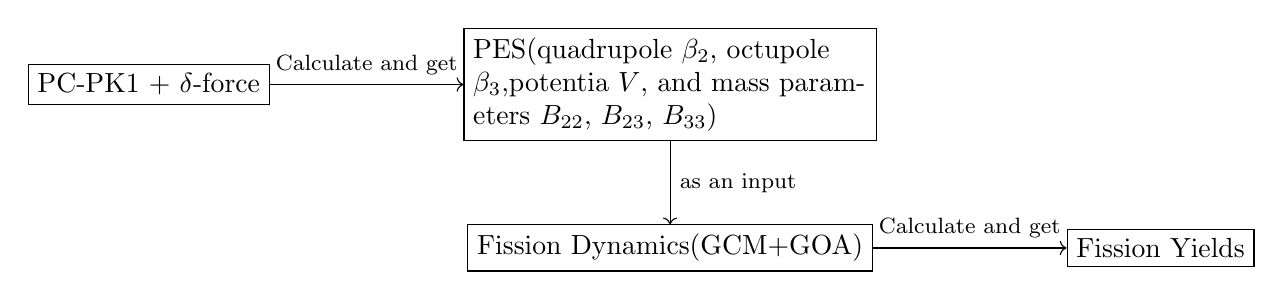
\begin{tikzpicture}[node distance=10pt]
                    \node[draw, text width=5cm]      (start)  {PES(quadrupole $\beta_2$, octupole $\beta_3$,potentia $V$, and mass parameters $B_{22}$, $B_{23}$, $B_{33}$)};
                    \node[draw, left=70pt of start]  (step1)  {PC-PK1 + $\delta$-force};
                    \node[draw, below=30pt of start] (step2)  {Fission Dynamics(GCM+GOA)};
                    \node[draw, right=70pt of step2] (step3)  {Fission Yields};

                    \draw[<-]  (start) -- node[above] {\footnotesize{Calculate and get}} (step1);
                    \draw[->] (start) -- node[right] {\footnotesize{as an input}} (step2);
                    \draw[->]  (step2) -- node[above] {\footnotesize{Calculate and get}} (step3);
                \end{tikzpicture}
                
            \item Coordinate   \newline
                $\hat{Q}_k$ denotes the expectation value of the mass quadrupole and the octupole operators
                \begin{equation}
                    \hat{Q}_2 = 2z^2 - r_{\bot}^2 \quad \text{and} \quad \hat{Q}_3 = 2z^3 - 3zr_{\bot}^2    \label{b1}
                \end{equation}
                The corresponding deformation parameters $\beta_2$ and $\beta_3$ can be determined from the following relations:
                \begin{equation}
                    \begin{aligned}
                        \beta_2 = \frac{\sqrt{5\pi}}{3AR_0^2}\langle \hat{Q}_2 \rangle,   \quad
                        \beta_3 = \frac{\sqrt{7\pi}}{3AR_0^3}\langle \hat{Q}_3 \rangle  \label{b2}  
                    \end{aligned}
                \end{equation}
                with $R_0 = r_0 A^{1/3}$ and $r_0 = 1.2{\rm fm}$.\newline
                \textbf{Example -- Phy.Rev.C 93, 054611 (2016)}\\
                The quadrupole and octupole moments in this article is 
                \begin{equation}
                    \hat{Q}_{20} = 2z^2 - r_{\bot}^2 \quad \text{and} \quad \hat{Q}_{30} = \sqrt{\frac{7}{4\pi}}(z^3 - zr_{\bot}^2) \label{b3}
                \end{equation}
                the unit for $\hat{Q}_{20}$ is $barn(b)$, we have $1b = 100fm^2$, and unit for $\hat{Q}_{30}$ is $b^{3/2}$, the definition is different from \eqref{b1}, according to \eqref{b1}-\eqref{b3}, we have the transformational relation 
                \begin{equation}
                    \begin{aligned}
                        \beta_2 = \frac{\sqrt{5\pi}}{3AR_0^2}\langle \hat{Q}_{20} \rangle,   \quad
                        \beta_3 = \frac{4\pi}{3AR_0^3}\langle \hat{Q}_{30} \rangle
                    \end{aligned}
                \end{equation}

            \item Strengths parameters of $\delta$-force    \\
                Using a five-point formula to cacluate the pairing gap parameters:
                \begin{equation}
                    \Delta_{q}^{(5)} (N_0) = -\frac{\pi_{N_0}}{8} \left[ E(N_0 + 2) - 4E(N_0 + 1) + 6E(N_0) - 4E(N_0 - 1) + E(N_0 -2) \right]
                \end{equation}
                where $\pi_{N_0} = (-1)^{N_0}$, $N_0$ reprecent numbers of protons or neutrons in the nuclei that we need to calculate.
            \item Neck Operator     \\
                \begin{equation}
                    \hat{Q}_N = exp\left[ \frac{-(z-z_n)^2}{a_N^2} \right]
                \end{equation}
                where $a_N = 1$fm and $z_N$ is the position of the neck[56].
            \item Total Kinetic Energy  \\
                \begin{equation}
                    E_{TKE} = \frac{e^2 Z_H Z_L}{d_{ch}}
                \end{equation}
                where $e$ is the proton charge, $Z_H(Z_L)$ is the charge of the heavy(light) fragment, $d_{ch}$ is the distance between fragment centers of charge at scission.
        \end{enumerate}

    \item \textbf{Result and Discussion}
        \begin{enumerate}[leftmargin=10pt]
            \item Pairing Strength    \newline
                The general topography of the PESs does not change significantly as pairing increases, the barriers are reduced considerably.   \newline
                %\noindent \includegraphics[width=7cm]{figure/literatures/reference-1_2.pdf} \newline
                As pairing correlations increase, the collective masses are reduced and the shell oscillations are also reduced. And the pattern of the scission line does not change significantly with the varience of the pairing strength.  \newline
                The pairing strength influence the fission yields significantly due to the reduction of the ridge between asymmetric and symmetric fission when increasing the pairing strength.
            \item Excitation Energy \newline
                With the increase in energy, the current can more directly enter the symmetric valle and, consequently, the asymmetric peaks are lowered while the symmetric peak gradually bcomes wider.
        \end{enumerate}
\end{itemize}

%%%%%%%%%%%%%%%%%%%%%%%%%%%%%%%%%%%%%%%%%%%%%%%%%%%%%%%%%%%%%%
\vspace{8pt}
\noindent\rule[0.25\baselineskip]{\textwidth}{2pt}
\noindent \textcolor{blue}{\textbf{[2] D. Regnier, N. Dubray and N. Schunck, From asymmetric to symmetric fission in the fermium isotopes within the time-dependent generator-coordinate-method formalism, Phy.Rev.C 99, 024611(2019)}}
\begin{itemize}[leftmargin=10pt]
    \item \textbf{Words}
    \begin{enumerate}[leftmargin=10pt]
        \item  \textcolor{red}{In heavy and superheavy nuclei, a difference of only a few neutrons is sufficient to change the dominant fission mode.}
        \item More recently, studies of static deformation properties of fermium isotopes were also performed within a self-consistent meanfield framework based on Gogny, Skyrme, and covariant energy density functionals (EDFs) [17-22]. All these papers emphasized the multimodal character of the fission of fermium isotopes near A = 256 and highlighted the presence of three major modes: symmetric compact, symmetric elongated, and asymmetric.
        \item In the TDGCM+GOA picture, the presence of valleys in the potential energy landscape favors the diffusion of the collective wave packet toward specific sets of configurations at scission.
        \item At $Q_{20}=140{\rm b}$, symmetric configurations are largely favored energetically in all three isotopes. 
    \end{enumerate}

    \vspace{5pt}
    \item \textbf{Note}
        \begin{enumerate}[leftmargin=10pt]
            \item Main Idea \newline
                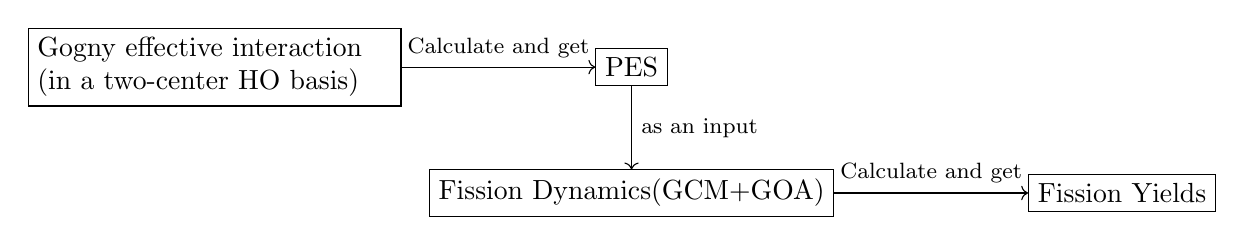
\begin{tikzpicture}[node distance=10pt]
                    \node[draw]                      (start)  {PES};
                    \node[draw, left=70pt of start, text width=4.5cm]  (step1)  {Gogny effective interaction \\ (in a two-center HO basis)};
                    \node[draw, below=30pt of start] (step2)  {Fission Dynamics(GCM+GOA)};
                    \node[draw, right=70pt of step2] (step3)  {Fission Yields};

                    \draw[<-]  (start) -- node[above] {\footnotesize{Calculate and get}} (step1);
                    \draw[->] (start) -- node[right] {\footnotesize{as an input}} (step2);
                    \draw[->]  (step2) -- node[above] {\footnotesize{Calculate and get}} (step3);
                \end{tikzpicture}
            \item Fission Mode  \newline
                symmetric compact fission mode[19, 21], symmetric elongated fission mode.   \newline
                The rapid decreasing of potential around $Q_{20} \simeq 220b$ is correspods to the symmetric fission mode.
            \item PES   \newline
                The potential ridge is indeed quite pronounced for $\prescript{258}{}{\rm Fm}$ but progressively disappears as we go toward the lighter isotopes.
            \item Fission Fragments Distributions   \newline
                Taking into account the \underline{neutron evaporation} would shift our predictoins by a few units toward lighter masses as well as bring additional structure and asymmetry between the light and heavy peaks.   \newline
                A second important effect that also impacts the comparison with experiment is the \underline{initial energy} of the fissioning system.
        \end{enumerate}
    \item My confusion
        \begin{enumerate}[leftmargin=10pt]
            \item \textcolor{red}{What is disentanglement of the fragment?}
        \end{enumerate}
    \item \textbf{\textcolor{red}{My Thinking}} \newline
        It may be important to analysis the potential variety along the $Q_{30}$ around the scission point when keeping $Q_{20}$ a constant(\textcolor{cyan}{see ${\rm \uppercase\expandafter{\romannumeral3}.A.2}$}).
\end{itemize}

%%%%%%%%%%%%%%%%%%%%%%%%%%%%%%%%%%%%%%%%%%%%%%%%%%%%%%%%%%%%%%
\vspace{8pt}
\noindent\rule[0.25\baselineskip]{\textwidth}{2pt}
\noindent \textcolor{blue}{\textbf{[3] Guillaume Scamps${}^*$, C{\' e}dric Simenel${}^{\dag}$, Denis Lacroix${}^{\ddag}$, Superfluid dynamics of $\prescript{258}{}{\rm Fm}$ fission, Phy.Rev.C 92, 011602(R)(2015)}}
\begin{itemize}[leftmargin=10pt]
    \item \textbf{Words}
        \begin{enumerate}[leftmargin=10pt]
            \item Indeed, magic fragments are difficult to excite and deform and, thus, fission occurs faster \textcolor{red}{as less dissipation is involved}, leading to a larger TKE.
        \end{enumerate}
        
\end{itemize}

%%%%%%%%%%%%%%%%%%%%%%%%%%%%%%%%%%%%%%%%%%%%%%%%%%%%%%%%%%%%%%
\vspace{8pt}
\noindent\rule[0.25\baselineskip]{\textwidth}{2pt}
\noindent \textcolor{blue}{\textbf{[4] W. Younes and D. Gogny, Nuclear Scission and Quantum Localization, Phys.R}}
\begin{itemize}[leftmargin=10pt]
    \item Essential Words
    \begin{enumerate}[leftmargin=10pt]
        \item The disentanglement of the fragment wave functions is essential to the quantum-mechanical definition of scission and the calculation of physical observables.
        \item Scission implies a separation of the nucleus into independent fragments, \textcolor{blue}{while the Pauli exclusion principle introduces a persistent correlation between the fragments, no matter how far apart they are.}
    \end{enumerate}

    \vspace{5pt}
    \item Some elegant Words
        \begin{enumerate}[leftmargin=10pt]
            \item 
        \end{enumerate}
    
    \vspace{5pt}
    \item My confusion
        \begin{enumerate}[leftmargin=10pt]
            \item \textcolor{red}{What is disentanglement of the fragment wave functions?}(reference [6])
            \item \textcolor{red}{What is the definition of the neck size?}(reference[9])
            \item \textcolor{red}{Where is the "tails"?}(reference[9])
            \item \textcolor{red}{Bogoliubov vacuum is only defined up to a unitary transformation of the qp destruction operators.}(Why?)
        \end{enumerate}
\end{itemize}

%%%%%%%%%%%%%%%%%%%%%%%%%%%%%%%%%%%%%%%%%%%%%%%%%%%%%%%%%%%%%%
\vspace{8pt}
\noindent\rule[0.25\baselineskip]{\textwidth}{2pt}
\noindent \textcolor{blue}{\textbf{[5] W. Younes and D. Gogny, Microscopic calculation of $\sideset{^{240}}{}{\mathop{\mathbf{Pu}}}$ scission with a finite-range effective force, Phy.Rev.C 80, 054313(2009)}}
\begin{itemize}[leftmargin=10pt]
    \item some useful points
    \begin{enumerate}[leftmargin=10pt]
        \item 
    \end{enumerate}
\end{itemize}

%%%%%%%%%%%%%%%%%%%%%%%%%%%%%%%%%%%%%%%%%%%%%%%%%%%%%%%%%%%%%%
\vspace{8pt}
\noindent\rule[0.25\baselineskip]{\textwidth}{2pt}
\noindent \textcolor{blue}{\textbf{[6] A. Zdeb, A. Dobrowolski and M. Warda, Fission dynamics of $^{252}Cf$, Phy.Rev.C 95, 054608(2017)}}
\begin{itemize}[leftmargin=10pt]
    \item  \textbf{Words}
    \begin{enumerate}[leftmargin=10pt]
        \item Calculat the PES by HFB model with the D1S Gogny-type interactions.
        \item Calculat the dynamic of fission within TDGCM+GOA formalism.
    \end{enumerate}
    \item Some points
    \begin{enumerate}[leftmargin=10pt]
        \item It has been shown that minimization of action integral with the nonperturbative mass parameters modifies the fission trajectory in the barrier region. The penetration probability is higher in comparison to that resulting from dynamic calculations within perturbative inertias.
    \end{enumerate}
\end{itemize}

%%%%%%%%%%%%%%%%%%%%%%%%%%%%%%%%%%%%%%%%%%%%%%%%%%%%%%%%%%%%%%
\vspace{8pt}
\noindent\rule[0.25\baselineskip]{\textwidth}{2pt}
\noindent \textcolor{blue}{\textbf{[7] J${\rm o\mkern-8.5mu/}$rgen Randrup and Ramona Vogt, Generation of Fragment Angular Momentum in Fission, Phy.Rev.L 127, 062502(2021)}}
\begin{itemize}[leftmargin=10pt]
    \item \textbf{Question}
    \item What \newline
        \underline{Binary character} prior to scission[12] \newline
        \underline{Six dinuclear rotational modes:} wriggling and bending(double degenerate), twisting and tilting[13,14]\newline
        What is the meaning of the setence \textcolor{red}{"In particula, expressions were derived for associated mobility coefficients which ... so it remains in local equilibrium."}\newline
        What is the \underline{statistical fluctuations} in angular momentum.
    \item \textbf{Words}
    \begin{enumerate}[leftmargin=10pt]
        \item 
    \end{enumerate}
    \begin{enumerate}[leftmargin=10pt]
        \item 
    \end{enumerate}
    \item \textbf{Some points}
    \begin{enumerate}[leftmargin=10pt]
        \item 
    \end{enumerate}
\end{itemize}

%%%%%%%%%%%%%%%%%%%%%%%%%%%%%%%%%%%%%%%%%%%%%%%%%%%%%%%%%%%%%%
\vspace{8pt}
\noindent\rule[0.25\baselineskip]{\textwidth}{2pt}
        \noindent \textcolor{blue}{\textbf{[8] N. Schunck and L.M. Robledo, Microscopic theory of nuclear fission: a review, Rep. Prog. Phys. 79(2016), 116301}}
\begin{itemize}[leftmargin=10pt]
    \item \textbf{Abstract}
        \begin{enumerate}[leftmargin=10pt]
            \item In \underline{spotaneous fission}, the half-lives are the main observables and quantum tunnelling the essential concept; in \underline{induced fission}, the focus is on fragment properties and explicitly time-dependent approaches are often invoked.
            \item Overall, the cornerstone of the density functional theory approch to fission is the energy density functional formalism.
        \end{enumerate}
    \item \textbf{Introduction}
        \begin{enumerate}[leftmargin=10pt]
            \item The nuclear 'fissility' parameter:
                \begin{equation}
                    x \approx \frac{Z^2}{50.88A(1-\eta I^2 )}
                \end{equation}
                where $I = (N - Z)/A$ and $\eta = 1.7826$ [6-8]. In the liquid drop model, the fissility is related to the ratio between the Coulomb and surface energy of the drop. for values of $x > 1$, the drop is unstabel against fission, and nulcear fission can then occur spontaneously.
            \item Nuclear fission also plays an important role in the formation of elements in the rapid neutron capture process(r-process) of nucleosynthesis in stellar environments.
            \item Because of the \underline{strong nuclear binding}, the energy released during fission is very large (compared to other energy production sources), typically of the order of 200 MeV per fission event. Most of it is kinetic energy of the fission fragments while about $10\sim 20\%$ of it is excitation energy. 
        \end{enumerate}
    \item \textbf{Potential energy surfaces} \newline
        The \textcolor{red}{cornerstone} of the implementation of the adiabatic approximation in fission theory is the definition of a \textcolor{red}{potential energy surface(PES)} in an arbitrary collective space. 
        \begin{enumerate}[leftmargin=10pt]
            \item \textcolor{cyan}{\underline{The macroscopic-microscopic approach}}\newline
                \underline{Main Idea:} The MM approach consists in viewing the nucleus as a finite chunk of nulcear matter, the energy of which is parametrized as a function of the charge, mass and deformations $\bm{q}$ of the nucleus.\newline
                \underline{Total Energy:} (i)$E_{mac}$ is the macroscopic energy obtained by a deformed liquid drop or droplet formula, represets bulk nuclear properties;(ii) a shell correction $E_{shell}$, accounts for the distribution of single particle levels in the average nuclear potential and thus has a one-body origin;(iii) a pairing correction $E_{pair}$, which has a two-body origin. The formation of the total energy is
                \begin{equation}
                    E(\bm{q}) = E_{mac}(\bm{q}) + E_{shell}(\bm{q}) + E_{pair}(\bm{q})
                \end{equation}
                In MM approach, we \textcolor{red}{first} formula a formulation to describe the nuclear shape, \textcolor{red}{then} we introduce some microscopic quantum corrections(just like shell, pairing correlation correction) in the macroscopic energy. 
                \begin{enumerate}
                    \item Parametrization of the nuclear surface \newline
                        The simplest and most common parametrization is based on the multipole expansion of the nuclear radius[56]:
                        \begin{equation}
                            R(\theta, \varphi)=R_{0} c(\alpha)\left[1+\sum_{\lambda \geqslant 2} \sum_{\mu=-\lambda}^{+\lambda} \alpha_{\lambda \mu} Y_{\lambda \mu}(\theta, \varphi)\right]
                        \end{equation}
                        where $R_0 = r_0 A^{1/3}$ is a parametrization of the nuclear radius for a spherical nulceus of mass $A(r_0 \approx 1.2 {\rm fm})$; $c(\alpha)$ is a factor accounting for the conservation of nuclear volume with deformation; the $\alpha_{\lambda\mu}$ are the deformation parameters; $Y_{\lambda\mu}(\theta,\phi)$ are the usual spherical harmonics.
                \end{enumerate}
        \end{enumerate}
    
\end{itemize}
%%%%%%%%%%%%%%%%%%%%%%%%%%%%%%%%%%%%%%%%%%%%%%%%%%%%%%%%%%%%%%
\vspace{8pt}
\noindent\rule[0.25\baselineskip]{\textwidth}{2pt}
        \noindent \textcolor{blue}{\textbf{[9] D. Regnier,${}^{1,*}$ N. Dubray,${}^{1,\dagger}$ N. Schunck, ${}^{2,\ddagger}$ and M. Verrière, Fission fragment charge and mass distribution in $\sideset{^{239}}{}{\mathop{\mathbf{Pu(n,f)}}}$ in the adiabatic nuclear energy density functional theory, Phy. Rev. C 93, 054611(2016)}}
\begin{itemize}[leftmargin=10pt]
    \item
\end{itemize}
%%%%%%%%%%%%%%%%%%%%%%%%%%%%%%%%%%%%%%%%%%%%%%%%%%%%%%%%%%%%%%
%%%%%%%%%%%%%%%%%%%%%%%%%%%%%%%%%%%%%%%%%%%%%%%%%%%%%%%%%%%%%%
\section{Density Functional}

\noindent\rule[0.25\baselineskip]{\textwidth}{2pt}
\noindent \textcolor{blue}{\textbf{[1] P.W. Zhao, Z.P. Li, J.M. Yao and J. Meng, New parametrization for the nuclear convariant energy density functional with a point-coupling interaction, Phy.Rev.C 82, 054319(2010)}}
\begin{itemize}[leftmargin=10pt]
    \item The main result of the theory
    \begin{enumerate}[leftmargin=10pt]
        \item The total energy for the nuclear system
        \begin{equation}
            E_{\mathrm{tot}}=E_{\mathrm{DF}}\left[\boldsymbol{\tau}, \rho_{S}, j_{i}^{\mu}, A_{\mu}\right]+ E_{\text {pair }}\left[\kappa, \kappa^{*}\right] + E_{\mathrm{c} . \mathrm{m} .}^{\mathrm{mic}}
        \end{equation}
        where the \textcolor{red}{center-of-mass(c.m.) correction energy } is
        \begin{equation}
            E_{\mathrm{c} . \mathrm{m} .}^{\mathrm{mic}} = -\frac{1}{2mA}\langle \hat{\boldsymbol{P}}^2_{c.m.} \rangle
        \end{equation}

    \end{enumerate}
\end{itemize}

\appendix
\chapter{变分原理及其应用}

%%%%%%%%%%%%%%%%%%%%%%%%%%%%%%
\section{变分原理}
在二维直角坐标中有两个定点$(x_1,\ y_1)$、$(x_2,\ y_2)$,连接这两点的任意一条曲线为$y = y(x)$,其满足边界条件如下:
\begin{equation}
    y(x_1) = y_1, \quad y(x_2) = y_2
\end{equation} 
现在,我们定义一个新的函数$f$,它是关于$y$和$y^{\prime}$($y$的一阶导数)的函数,形式为$f = f(y, y^{\prime})$,我们对其做关于$x$的定积分,如下
\begin{equation}
	I = \int_{x_1}^{x_2} f(y, y^{\prime}) \, dx	\label{eq:variation-simple}
\end{equation} 
这样,当$y$变化时,定积分$I$也会随之改变,这样,我们期望能找到某一个$y$,使$I$有极值(极大或极小)。

我们回顾一下以往的极值问题,对于某一个函数$y=y(x)$,我们变化自变量$x$,通过对比不同$x$处的函数值$y$来找到极值;现在我们来看式\eqref{eq:variation-simple},它的积分变量是$x$,且积分区间固定,我们无法通过改变$x$来改变$I$的值,但是被积函数$f$是关于$y$和$y^{\prime}$的函数,它的形式并不确定,因此,针对式$\eqref{eq:variation-simple}$的变分问题,我们考察的是:取不同形式的$y(x)$,使积分$I$有极值。\CJKunderdot{\textcolor{red}{我们习惯上把$I$称作$y(x)$的泛函}}【也就是函数的函数,$f$是$y$的函数,$I$是$f$的函数;或者$y$是$x$的函数($x$变化范围,例如从$x=1$变为$x=2$),$I$是$y$的函数($y$变换形式,如$y=x$变为$y=x^2$)】。由于取的是$I$的极值,因此当我们对$y(x)$做微小的变化是,$I$在一级近似下应该不变(也就是$I$关于$y$的一阶导为0)。$\delta y$是$y$的无穷小变化,习惯上把\CJKunderdot{\textcolor{red}{$\delta y$称为$y$的变分}}。

当我们变化$\delta y$时,$f$的变化为
\begin{equation}
	\delta f = \frac{\partial f}{\partial y} \delta y + \frac{\partial f}{\partial y^{\prime}} \delta y^{\prime}
\end{equation} 
$I$相应的变化为
\begin{equation}
	\delta I = \int_{x_1}^{x_2} \delta f \, dx = \int_{x_1}^{x_2} \left[  \frac{\partial f}{\partial y} \delta y + \frac{\partial f}{\partial y^{\prime}} \delta y^{\prime} \right] \, dx	\label{eq:variation}
\end{equation} 
方括号第二项用分部积分方法
\begin{equation}
	\begin{aligned}
		\int_{x_1}^{x_2} \frac{\partial f}{\partial y^{\prime}} \delta y^{\prime}\, dx =&{} \int_{x_1}^{x_2} \frac{\partial f}{\partial y^{\prime}} \left( \frac{d (\delta y)}{dx} \right) \, dx = \int_{x_1}^{x_2} \frac{\partial f}{\partial y^{\prime}} \, d (\delta y)	\\
		=&{} \left. \left( \frac{\partial f}{\partial y^{\prime}} \delta y \right) \right|_{x_1}^{x_2} - \int_{x_1}^{x_2} \delta y \frac{d}{dx}\left( \frac{\partial f}{\partial y^{\prime}} \right) \, dx
	\end{aligned}
\end{equation} 
考虑到边界是固定的,也就是在$x=x_1$和$x=x_2$出函数值$y(x_1)$和$y(x_2)$保持不变,因此我们有$\delta y(x_1) = \delta y(x_2) = 0$,上式最后一个等号右边第一项为0,即
\begin{equation}
	\left[ \frac{\partial f}{\partial y^{\prime}} \delta y \right]_{x_1}^{x_2} = 0
\end{equation}
将以上两式带回到式\eqref{eq:variation},得到
\begin{equation}
	\delta I = \int_{x_1}^{x_2} \left[ \frac{\partial f}{\partial y} - \frac{d}{dx}\left( \frac{\partial f}{\partial y^{\prime}} \right) \right] \, dx
\end{equation} 
若要求$I$有极值,则$\delta I = 0$,那么有下式成立
\begin{equation}
    \frac{\partial f}{\partial y} - \frac{d}{dx}\left( \frac{\partial f}{\partial y^{\prime}} \right) = 0
\end{equation} 
上式则是\textcolor{red}{Euler-Lagrange方程}。

\section{变分原理与Schr\"{o}dinger方程}
我们可以从变分原理出发,推导出Schr\"{o}dinger方程。

体系的Hamilton量为$\hat{H}$,




\end{document}
